\documentclass[11pt,a4paper]{article}
\usepackage[margin=2.5cm]{geometry}
\usepackage{amsmath,amssymb,bm}
\usepackage{graphicx}
\usepackage{float}
\usepackage{listings}
\usepackage{xcolor}
\usepackage{subcaption}
\usepackage{booktabs}
\usepackage[hidelinks]{hyperref}
\graphicspath{{figures/}}

\lstset{language=Python,basicstyle=\ttfamily\small,breaklines=true,frame=single}

% Anything you still have to write shows up in red so it can't be missed.
\newcommand{\todo}[1]{\textcolor{red}{[TODO: #1]}}

\title{Image Analysis: Home Exam}
\author{Elina Rosato}
\date{\today}

\begin{document}

\begin{titlepage}
    \centering
    \vspace*{2cm}

    {\Large Lund University\par}

    \vspace{1.5cm}

    {\large Course code: FMAN20\par}
    {\large Course name: Image Analysis\par}

    \vspace{3cm}

    {\Huge\bfseries Home Exam\par}

    \vspace{3cm}

    {\large\itshape Elina Rosato\par}

    \vspace{2cm}

    \begin{tabular}{rl}
        Program: & MSc Program in Machine Learning, Systems and Control \\[4pt]
        Lecturer: & K. Magnus J. Oskarsson
    \end{tabular}

    \vfill

    {\large \today\par}
\end{titlepage}

%==============================================================
\section{Task 1: Finding the odd toucan}
%==============================================================

\textbf{Task.} The image shows illustrated toucans (labelled A--H, eight in total) on a green background with a light-blue sky. They are identical except for one, where the eyelid is slightly different. The goal is to find that bird automatically.

\textbf{Approach in short.} The photo is a picture of a printed page, so it has uneven lighting, a shadow along the right edge and a slightly curved page. We therefore first cut the birds out of the background, and then compare local image features between the birds instead of comparing pixels. The pipeline is:

\begin{enumerate}
    \item Remove the background.
    \item Find the eight bird blobs.
    \item Crop each bird and compute SIFT descriptors.
    \item Score each bird by how badly its descriptors match the other birds. The highest score is the odd bird.
\end{enumerate}

\begin{figure}[H]
    \centering
    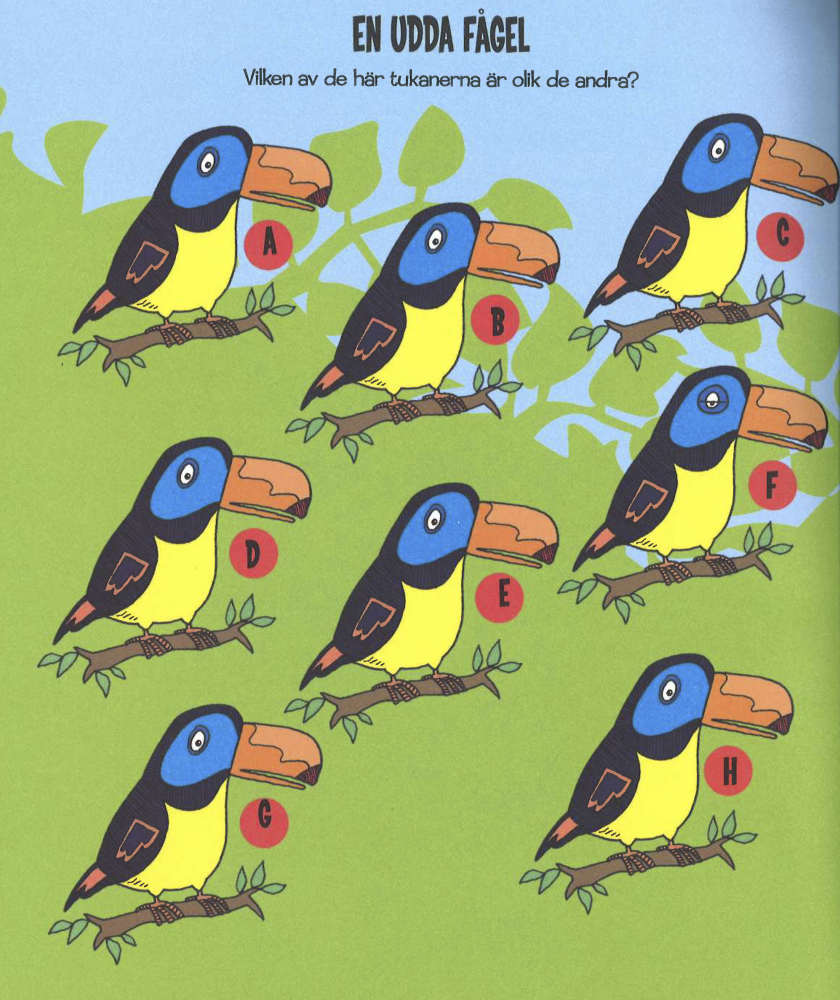
\includegraphics[width=0.45\textwidth]{00_original.png}
    \caption{Input image.}
\end{figure}

%--------------------------------------------------------------
\subsection{Step 1: Removing the background}
%--------------------------------------------------------------

The background is removed in three parts: first the green background, then the light-blue sky, and finally a clean-up that combines the two masks and removes the thin leaf outlines that would otherwise join the birds together.

\paragraph{Why HSV.} OpenCV loads the image as BGR. We convert it to HSV (hue, saturation, value) for the thresholding. In RGB, one colour such as green changes in all three channels when the brightness changes. In HSV the \emph{hue} channel describes the colour itself, independent of lighting, so a threshold like ``hue between 35 and 43 is green'' is stable against shadows and paper texture. Saturation and value are then used to separate colours that have similar hue.

\subsubsection{Green background}

\paragraph{Threshold.} The ranges for the thresholds were found by trial and error: we started from a typical range for the colour and adjusted the lower and upper limits, checking the resulting mask each time, until the background was removed without removing parts of the birds. The final green range is hue 35--43, saturation 105--210 and value at least 90. The lower saturation limit and the upper hue limit are what keep the leaves on the branches, which are a slightly different green, out of the background mask.

\paragraph{Cleaning the mask.} The raw mask has small holes from noise and paper texture. A \emph{morphological closing} (dilation followed by erosion) with a $5\times5$ kernel fills them. Then we compute the \emph{connected components} of the mask (each separate group of green pixels gets its own label) and keep only components larger than 6000 pixels. The large exterior background is kept. The small green patches, for example leaves on the branches that happen to have a similar colour, are discarded and stay part of the bird mask.

\begin{figure}[H]
    \centering
    \begin{subfigure}{0.32\textwidth}
        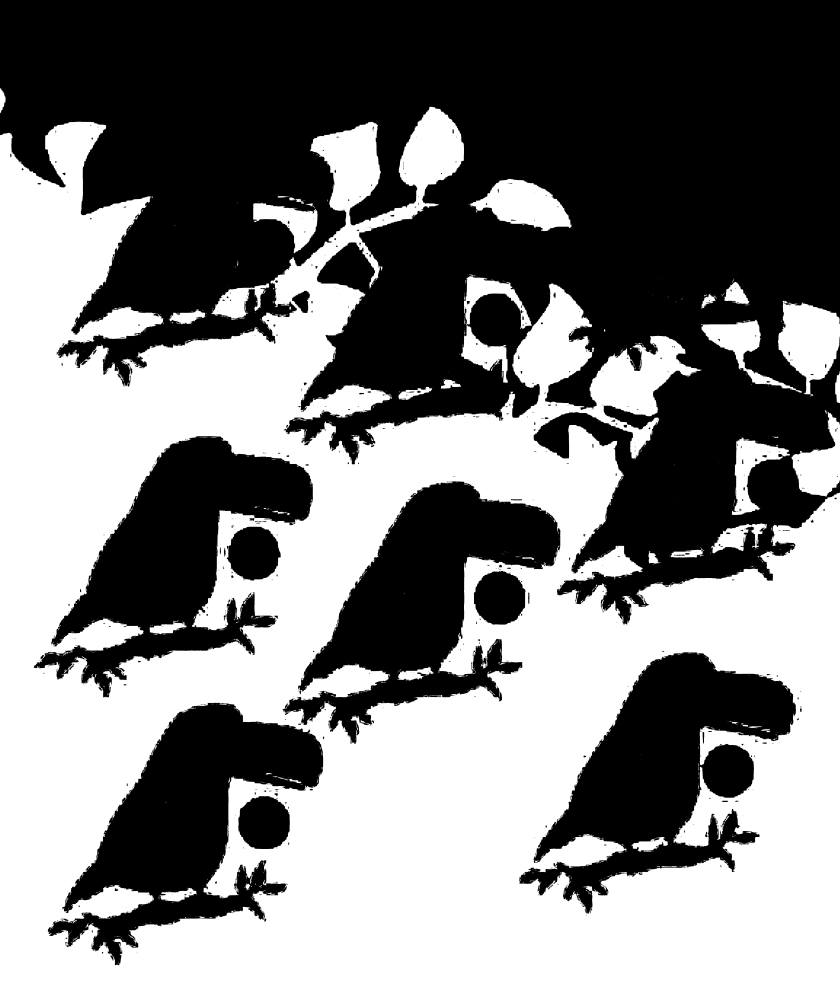
\includegraphics[width=\textwidth]{green_1_mask.png}
        \caption{HSV threshold}
    \end{subfigure}
    \begin{subfigure}{0.32\textwidth}
        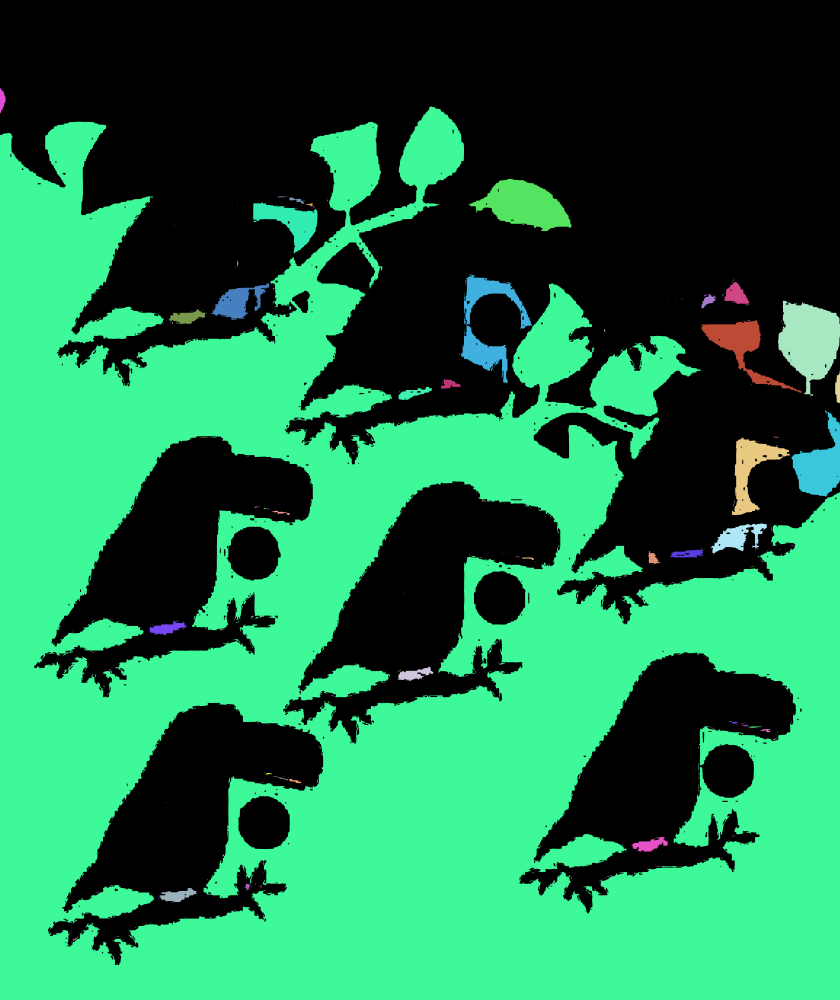
\includegraphics[width=\textwidth]{green_3_components.png}
        \caption{Connected components (one colour each)}
    \end{subfigure}
    \begin{subfigure}{0.32\textwidth}
        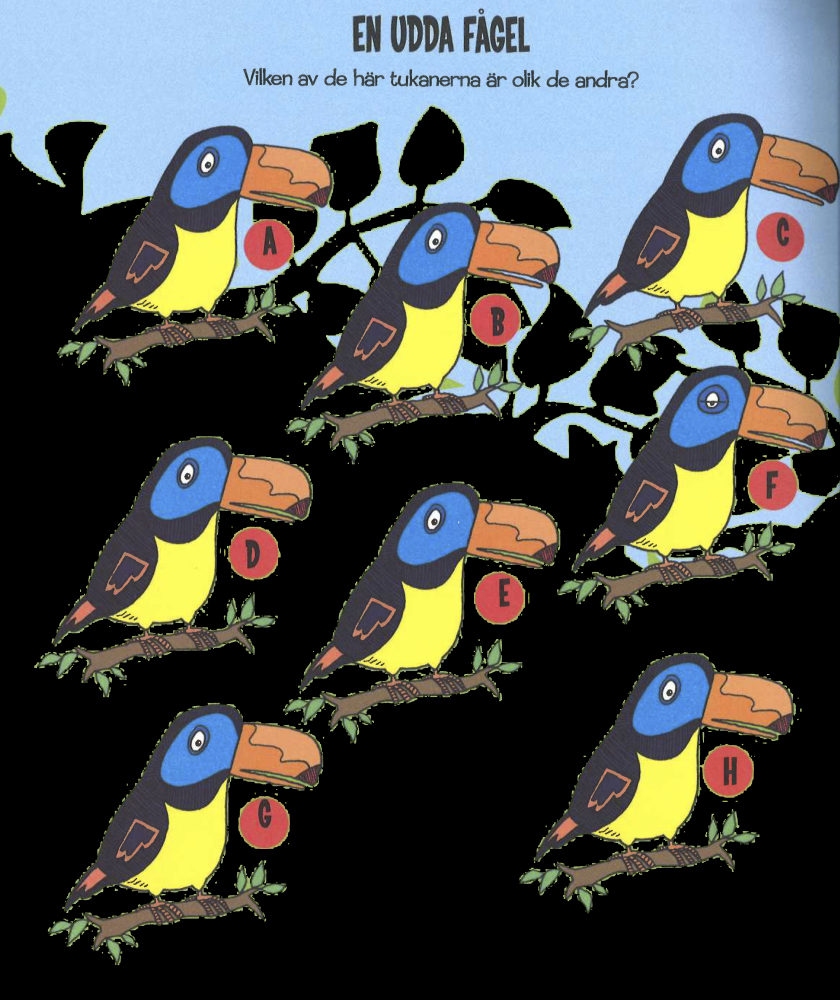
\includegraphics[width=\textwidth]{green_6_birds_only.png}
        \caption{Image with the green background removed}
    \end{subfigure}
    \caption{Green background removal.}
\end{figure}

%--------------------------------------------------------------
\subsubsection{Light-blue sky}
%--------------------------------------------------------------

The same procedure is applied to the light-blue sky between the leaves, and the limits were again found by trial and error. The final range is hue 85--115, saturation 25--100 and value at least 150, with a minimum component area of 1000 pixels.

The sky and the bird heads are both blue, so the hue alone cannot separate them. The upper saturation limit of 100 is what keeps the strongly coloured heads, and the dark blue ring around each eye, out of the sky mask. With looser limits the sky mask cut into the eyes, which is exactly the region we want to compare later.

\begin{figure}[H]
    \centering
    \begin{subfigure}{0.32\textwidth}
        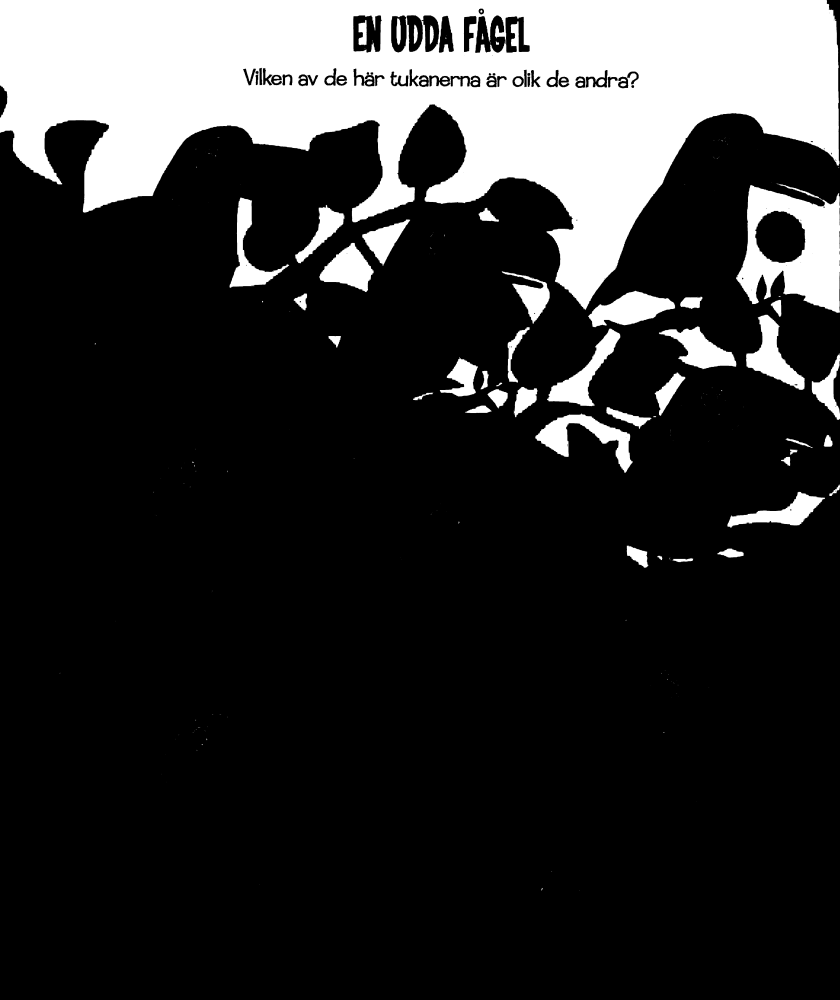
\includegraphics[width=\textwidth]{blue_1_mask.png}
        \caption{HSV threshold}
    \end{subfigure}
    \begin{subfigure}{0.32\textwidth}
        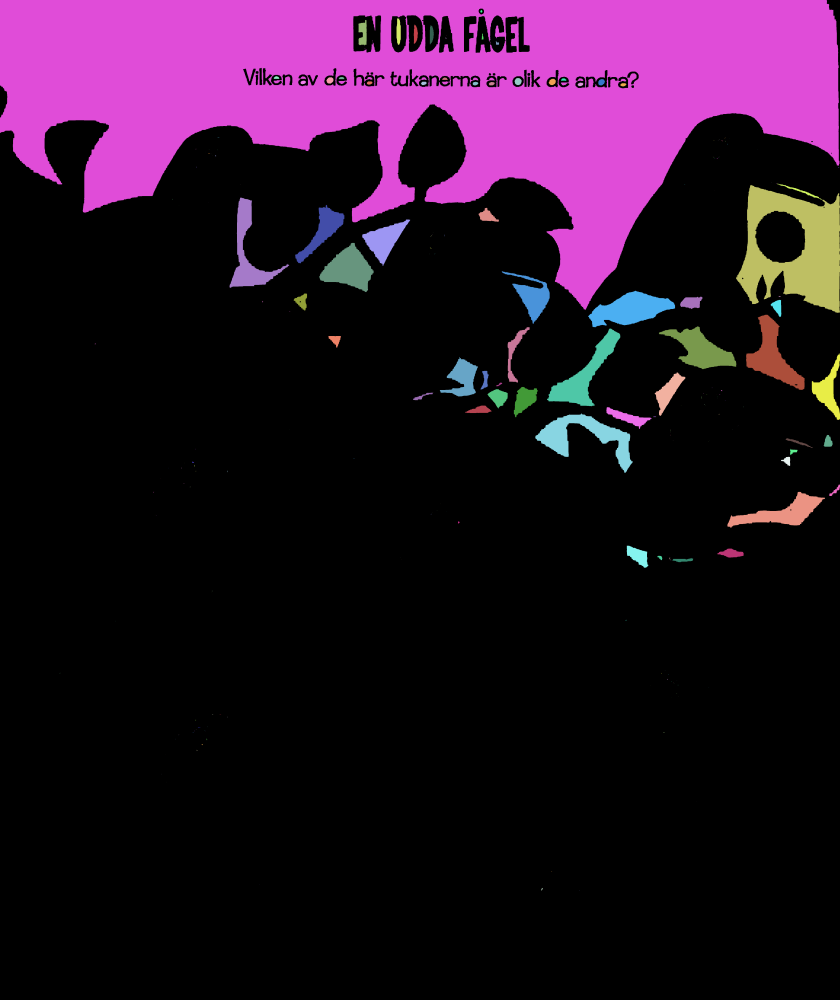
\includegraphics[width=\textwidth]{blue_3_components.png}
        \caption{Connected components}
    \end{subfigure}
    \begin{subfigure}{0.32\textwidth}
        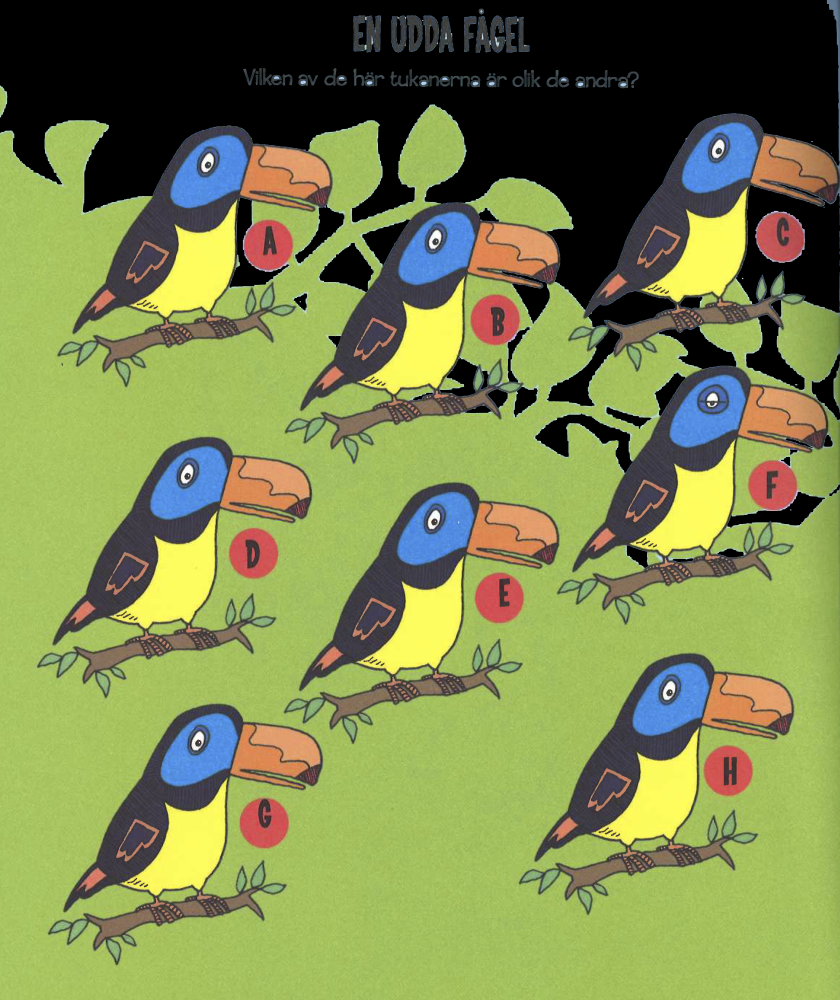
\includegraphics[width=\textwidth]{blue_6_birds_only.png}
        \caption{Image with the sky removed}
    \end{subfigure}
    \caption{Light-blue sky removal.}
\end{figure}

%--------------------------------------------------------------
\subsubsection{Combining the masks and removing the leaf outlines}
%--------------------------------------------------------------

A pixel is kept as a bird pixel only if it survived \emph{both} removals, so it is neither green nor blue. The result contains the birds and branches, but also the thin dark outlines of the background leaves. These outlines have colours between green and blue, so neither threshold removes them, and they form a network that connects neighbouring birds into one large blob.

A \emph{morphological opening} (erosion followed by dilation) with a $15\times15$ kernel fixes this. The erosion removes everything thinner than the kernel, which includes the outlines, and the dilation grows the large shapes back to roughly their original size. The birds are hundreds of pixels thick, so they survive, and the outlines do not. We use an opening on the \emph{bird} mask, since an opening removes thin white structures. (Opening the background mask would do the opposite.)

\begin{figure}[H]
    \centering
    \begin{subfigure}{0.4\textwidth}
        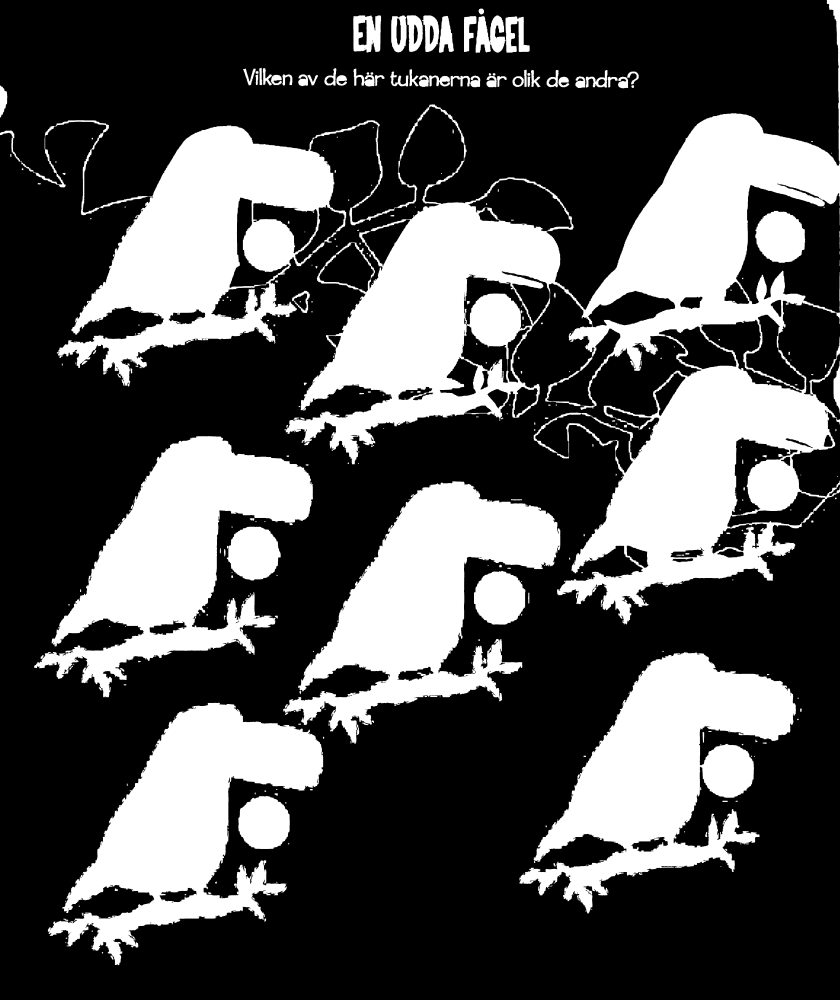
\includegraphics[width=\textwidth]{final_bird_mask.png}
        \caption{Combined bird mask}
    \end{subfigure}
    \begin{subfigure}{0.4\textwidth}
        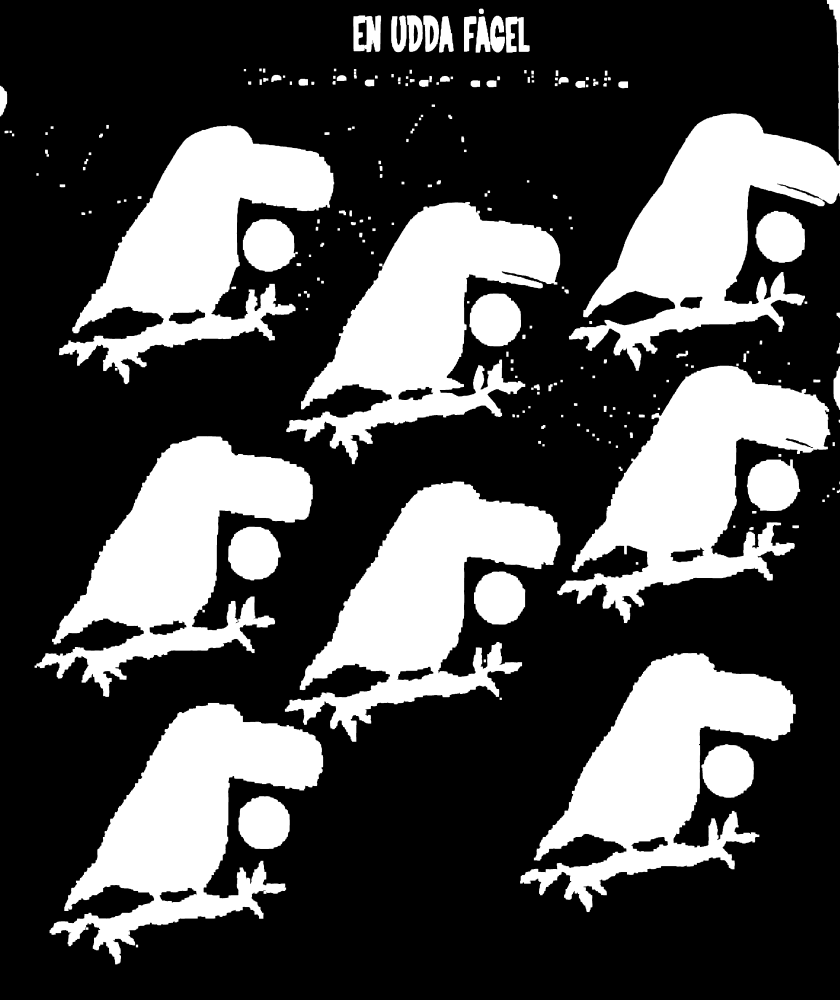
\includegraphics[width=\textwidth]{final_bird_mask_opened.png}
        \caption{After opening}
    \end{subfigure}
    \caption{Combined mask before and after the morphological opening.}
\end{figure}

\begin{figure}[H]
    \centering
    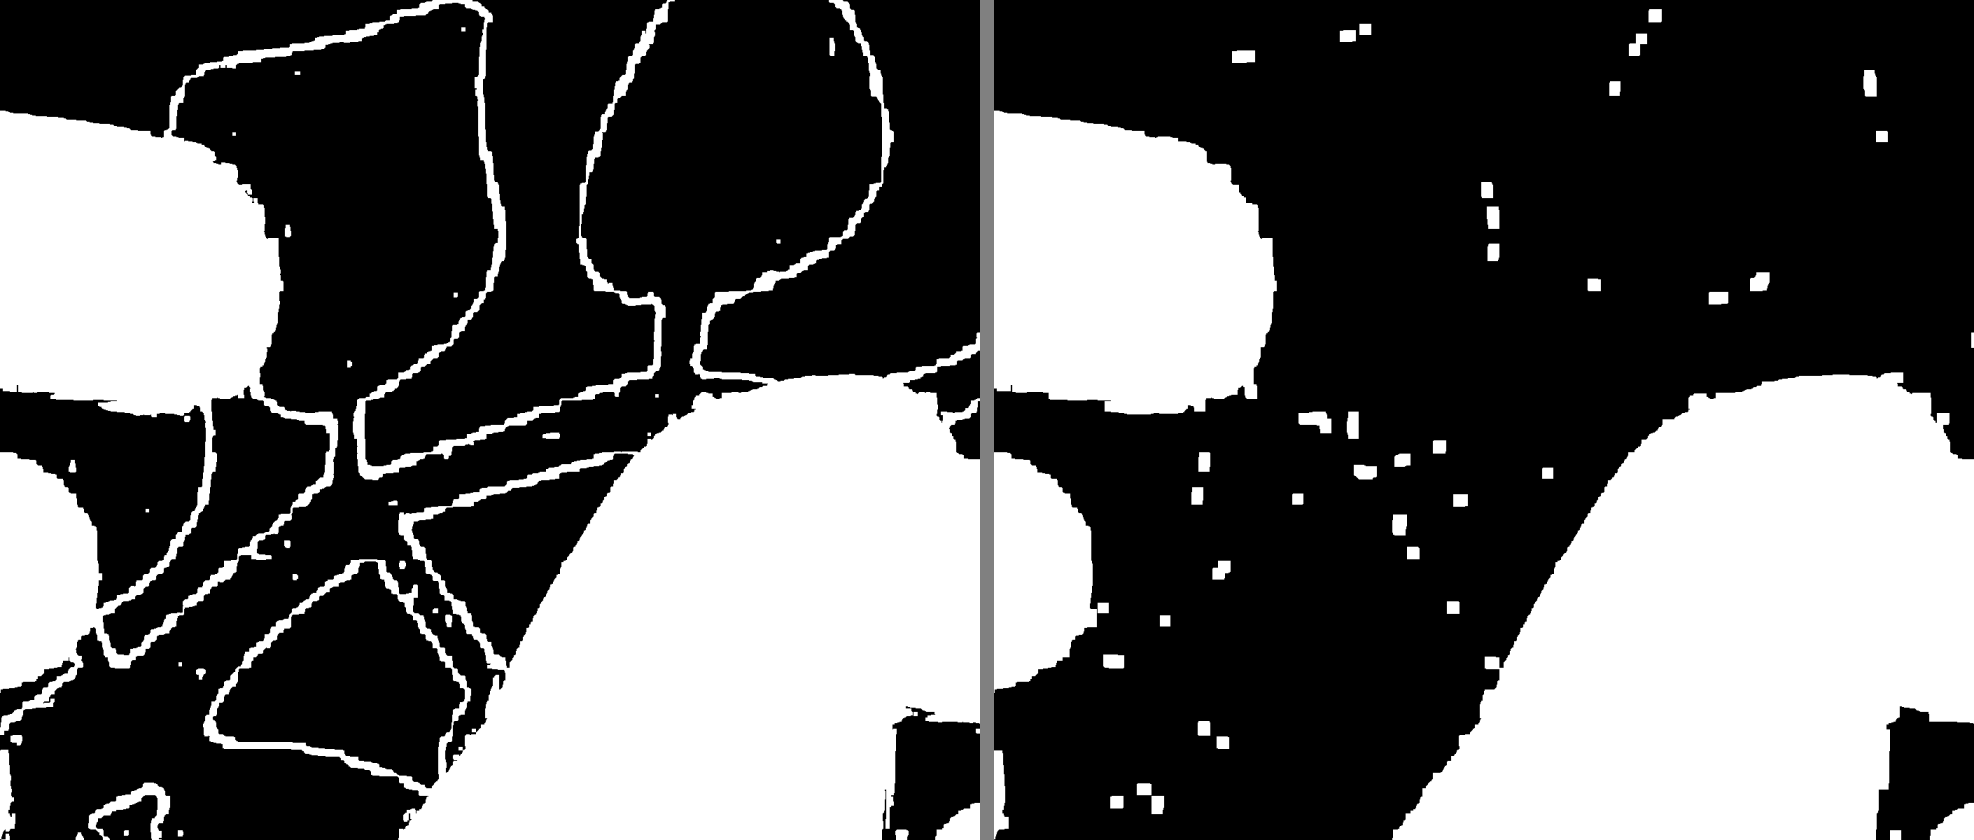
\includegraphics[width=0.9\textwidth]{opening_zoom.png}
    \caption{Zoom on the region between two birds. Left: the leaf outlines form a network that connects the birds. Right: after the opening only a few isolated specks remain, and these are removed by the area filter in the next step.}
\end{figure}

%--------------------------------------------------------------
\subsection{Step 2: Finding the bird blobs}
%--------------------------------------------------------------

We compute the connected components of the opened mask and sort them by area. The eight birds are about 1.2 million pixels each. The next largest component is only about 95\,000 pixels, so the eight largest components are the birds, and everything else is residual noise. Only these eight are kept. The kept mask is applied to the original image.

\begin{figure}[H]
    \centering
    \begin{subfigure}{0.4\textwidth}
        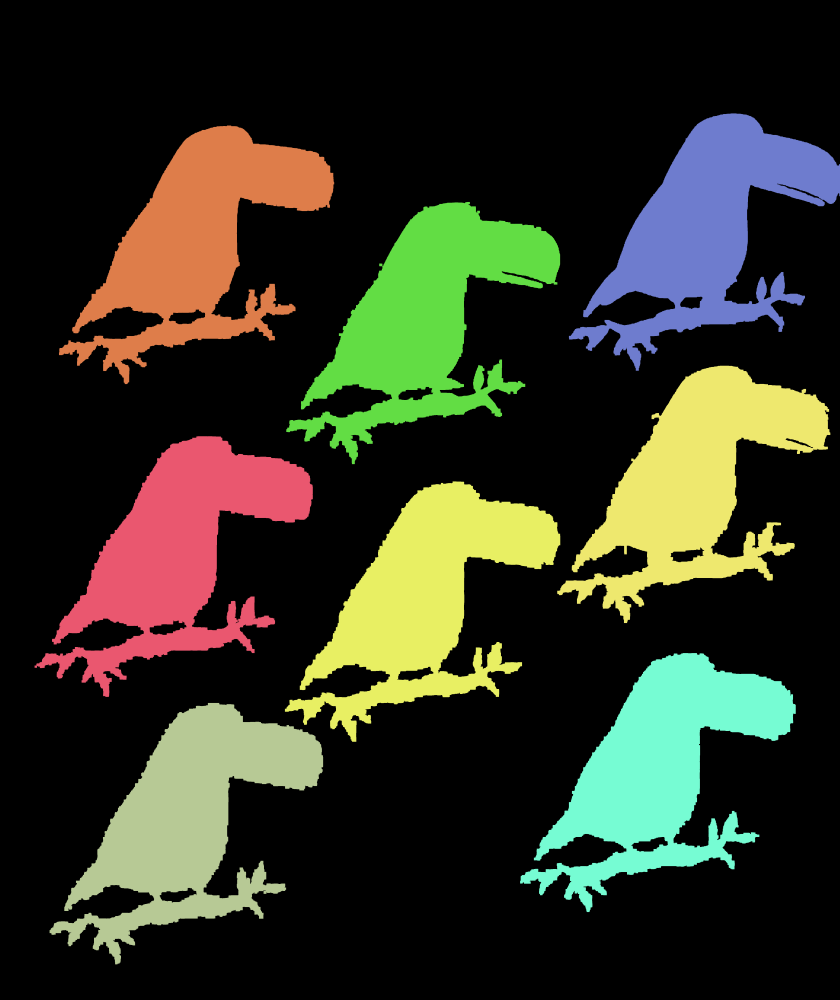
\includegraphics[width=\textwidth]{final_bird_blobs.png}
        \caption{The eight kept components}
    \end{subfigure}
    \begin{subfigure}{0.4\textwidth}
        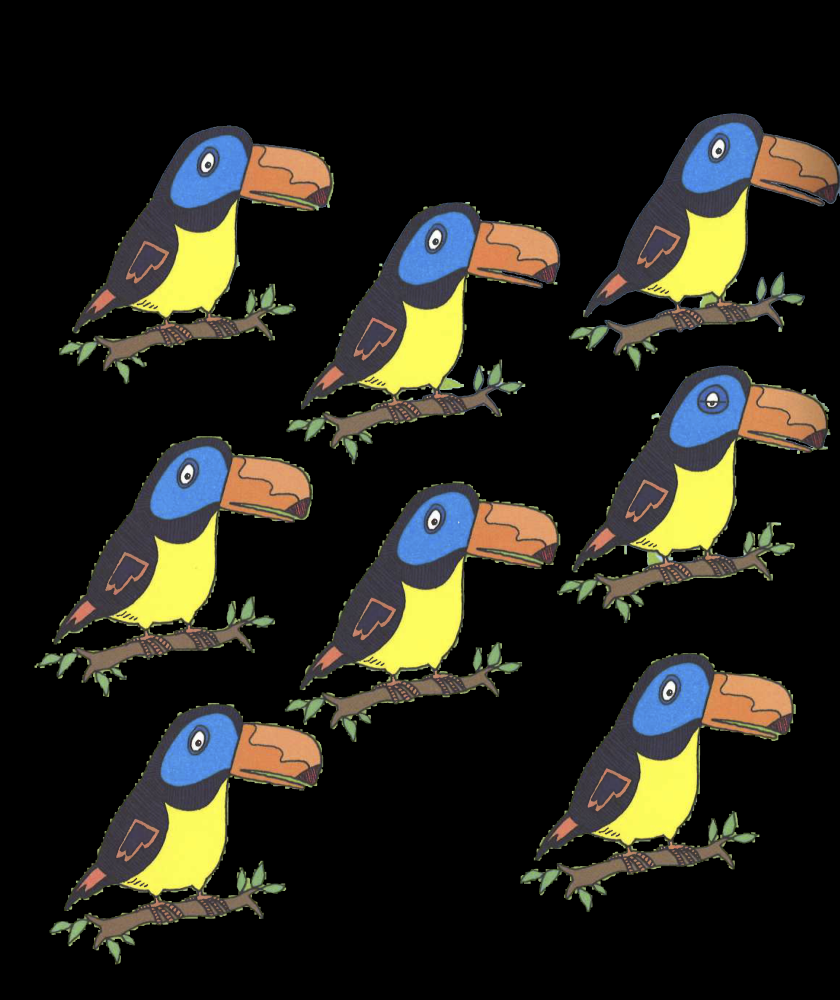
\includegraphics[width=\textwidth]{final_birds_masked.png}
        \caption{Final mask applied to the image}
    \end{subfigure}
    \caption{Result of the segmentation.}
\end{figure}

%--------------------------------------------------------------
\subsection{Step 3: Comparing the birds with SIFT}
%--------------------------------------------------------------

Our first attempt aligned all birds on top of each other and took the pixel difference to a median bird. This was misleading. The photo is of a book page, so shadow, curved paper and perspective change colours and positions slightly, and the bird closest to the page edge was reported as the odd one. We therefore compare local features, which are much less sensitive to this.

SIFT finds \emph{keypoints}, places in the image that are easy to recognise again, such as corners and edges. For each keypoint it computes a \emph{descriptor}, a vector of 128 numbers describing the directions of the image gradients around it. Descriptors are normalised for brightness and contrast, and are built to be invariant to scale and rotation. Two descriptors that describe the same detail look similar (small L2 distance), even if the lighting differs. Because of this we do not need to align the birds before comparing them.

For each of the eight blobs we crop the bounding box from the original image, set all pixels that do not belong to this bird to black, and resize so that the longest side is 800 pixels (keeping the aspect ratio). Before running SIFT the bird mask is \emph{eroded} with a $31\times31$ kernel, which shrinks it by about 15 pixels on every side. Cutting out a bird leaves a sharp artificial edge, and SIFT would place keypoints on it. These do not describe the bird, so we only search for keypoints inside the eroded region. SIFT is run on the grayscale image.

\begin{figure}[H]
    \centering
    \begin{subfigure}{0.28\textwidth}
        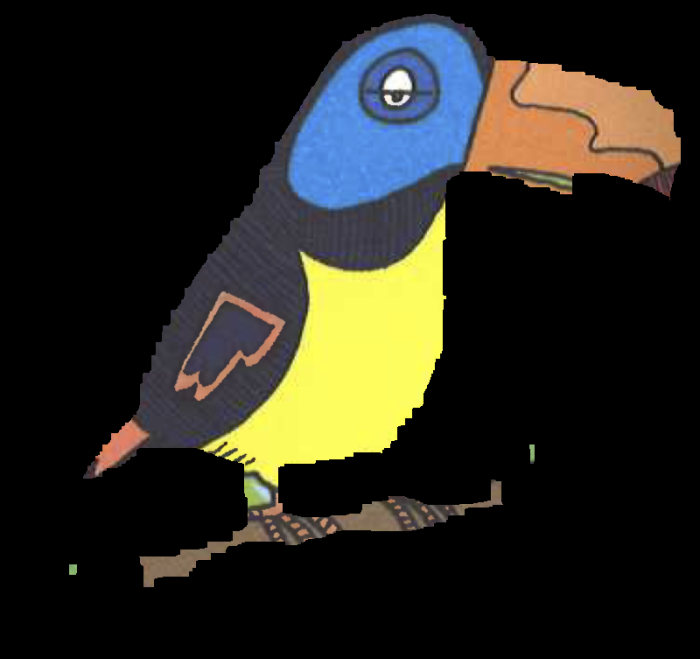
\includegraphics[width=\textwidth]{bird_6_1_eroded.png}
        \caption{Bird cut out with the eroded mask}
    \end{subfigure}
    \begin{subfigure}{0.28\textwidth}
        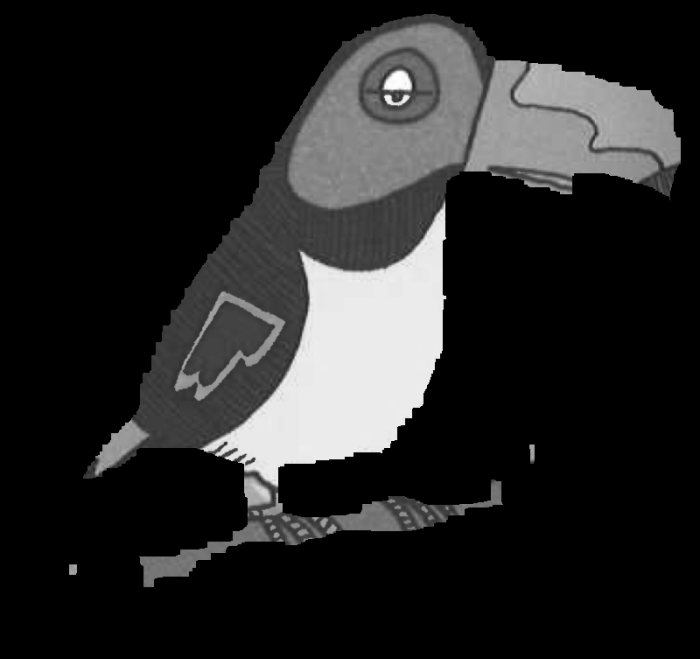
\includegraphics[width=\textwidth]{bird_6_2_gray.png}
        \caption{Grayscale image given to SIFT}
    \end{subfigure}
    \begin{subfigure}{0.28\textwidth}
        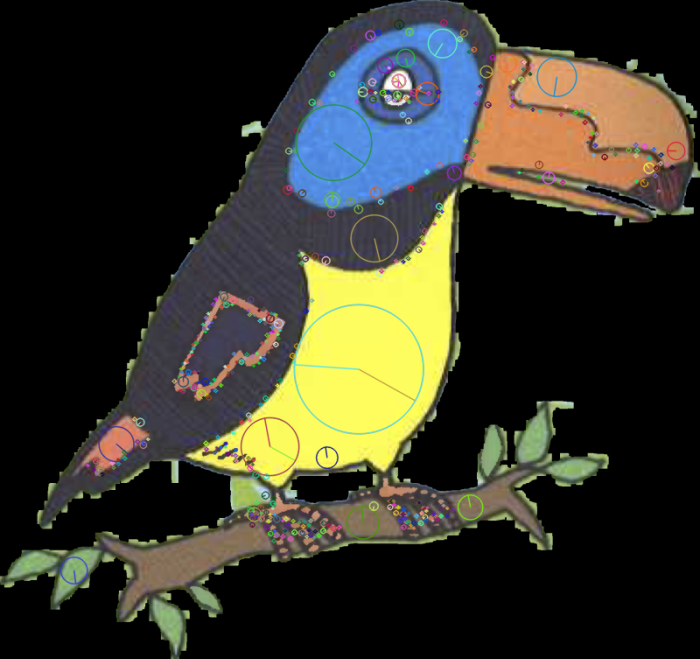
\includegraphics[width=\textwidth]{bird_6_3_keypoints.png}
        \caption{Detected keypoints}
    \end{subfigure}
    \caption{Preparation of one bird (bird F). Circles show the keypoints; their size and line show the scale and orientation.}
\end{figure}

\paragraph{Scoring.} For bird $i$ we pool the descriptors of all the other seven birds into one set. For each descriptor of bird $i$ we find the nearest descriptor in this set (brute-force L2 distance). If the other birds contain a similar detail the distance is small. If bird $i$ has a feature that none of the others have, such as a different eyelid, the distance is large. The score of bird $i$ is the mean of the $k$ largest distances:
\[
\text{score}(i) = \frac{1}{k}\sum_{\text{$k$ largest}} d_{\min}, \qquad k = \max\!\left(1,\ \lfloor 0.03\,N_i \rfloor\right),
\]
where $N_i$ is the number of keypoints in bird $i$. The bird with the highest score is the odd one out.

We use only the worst 3\,\% because the eyelid is a small detail that changes only a few keypoints. Averaging over all keypoints would hide these few among the hundreds that match well. Pooling the other birds gives each descriptor seven chances to find a match, so only features that are missing from the whole group give a large distance.

%--------------------------------------------------------------
\subsection{Result}
%--------------------------------------------------------------

\begin{center}
\begin{tabular}{lcc}
\toprule
Bird & Position in the image & Score \\
\midrule
\textbf{F} & right, middle & \textbf{380.2} \\
C & top right & 358.3 \\
E & centre & 324.6 \\
D & left, middle & 322.0 \\
G & bottom left & 319.7 \\
H & bottom right & 316.3 \\
B & top, centre & 303.6 \\
A & top left & 292.4 \\
\bottomrule
\end{tabular}
\end{center}

\textbf{Bird F} has the highest score and is correctly identified as the odd one: its eyelid is the feature that the other seven birds do not have.

The margin to the second bird (C, 358.3) is about 6\,\%. This is clear but not large. Bird C is the other bird closest to the page edge, where the shadow and the page curvature are strongest, which is the likely reason why its score is also raised.

%==============================================================
\section{Task 2: Histogram equalization}
%==============================================================

Throughout, $r$ is the input gray-level and $s=T(r)$ the output gray-level, both in $[0,1]$. A monotonically increasing transformation $T$ maps the fraction of pixels below $r$ to the same fraction of pixels below $s$, so
\begin{equation}
    \int_0^{s} p_{\text{out}}(u)\,du \;=\; \int_0^{r} p(t)\,dt .
    \label{eq:cdf}
\end{equation}

\subsection*{a) Threshold level for the input image}

Ordinary histogram equalization uses $T(r)=\int_0^r p(t)\,dt$. For $p(r)=3r^2$,
\[
    T(r) = \int_0^r 3t^2\,dt = r^3 .
\]
Thresholding the output at $0.5$ keeps the pixels with $T(r) > 0.5$. Since $T$ is increasing, this is the same as thresholding the input at the $r$ where $T(r)=0.5$:
\[
    r^3 = 0.5 \quad\Longrightarrow\quad r = 0.5^{1/3} = 2^{-1/3} \approx 0.794 .
\]
So the input image should be thresholded at gray-level $r \approx 0.794$.

\subsection*{b) Desired output distribution $p(s)=2s$}

The left side of (\ref{eq:cdf}) with $p_{\text{out}}(u)=2u$ is
\[
    \int_0^s 2u\,du = s^2 .
\]
Hence $s^2 = \int_0^r p(t)\,dt$, and the transformation is
\[
    T(r) = \sqrt{\int_0^r p(t)\,dt}\, .
\]
That is, the usual equalization transformation, followed by a square root. (The inverse is well defined since $s \in [0,1]$ and $s^2$ is increasing there.)

\subsection*{c) Input distribution $p(r)=6r(1-r)$ and output $p(s)=2s$}

The cumulative distribution of the input is
\[
    \int_0^r 6t(1-t)\,dt = 3r^2 - 2r^3 .
\]
Using the result of b),
\[
    T(r) = \sqrt{3r^2 - 2r^3} = r\sqrt{3-2r}\, .
\]

%==============================================================
\section{Task 3: Finding Olle's shadow}
%==============================================================

\textbf{Task.} The image shows a man in the middle and six purple silhouettes (labelled A--F). Only one silhouette is the shadow of the man. The goal is to find it automatically. A second image, with a patterned fabric background, is given as a harder case.

\textbf{Approach in short.} The man and the silhouettes are segmented from the background. Each silhouette is then compared to the man's silhouette with a mismatch score that tolerates small misalignments, and the silhouette with the lowest score is the answer. The pipeline is:
\begin{enumerate}
    \item Find the six silhouettes with a threshold on the purple colour.
    \item Find the man's silhouette by thresholding the colour of the background and removing it.
    \item Compare every silhouette with the man's silhouette.
\end{enumerate}

\begin{figure}[H]
    \centering
    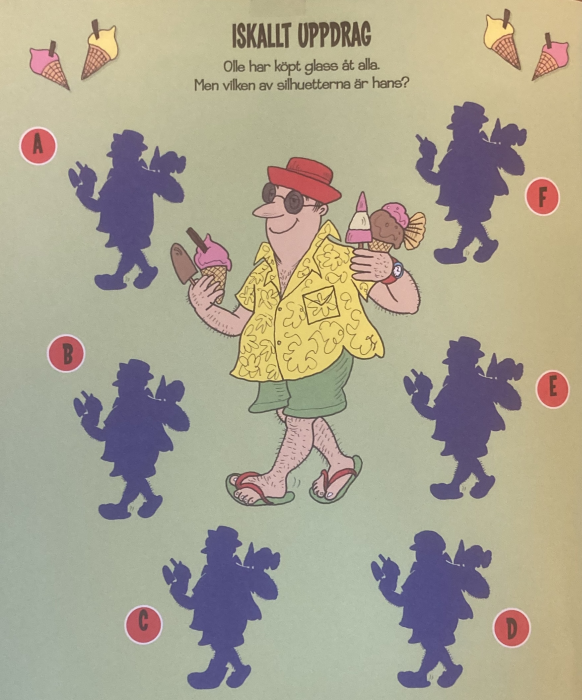
\includegraphics[width=0.45\textwidth]{t3_original.png}
    \caption{Input image.}
\end{figure}

%--------------------------------------------------------------
\subsection{Step 1: Finding the silhouettes}
%--------------------------------------------------------------

As in Task 1, the image is converted to HSV and thresholded. The silhouettes all have the same purple colour, so one range is enough: hue 105--150, saturation 40--150 and value 50--200. The range was found by trial and error, by adjusting the limits until all six silhouettes were fully selected. A tight range left one silhouette ragged on its right side, where the page is darker, so the range is fairly wide. Nothing else in the image has this colour.

The connected components of the mask are computed, and we keep the six largest, since we know there are six silhouettes. They are about 75\,000 to 84\,000 pixels each, while the largest leftover component is under 100 pixels, so there is no doubt about which six to take.

\begin{figure}[H]
    \centering
    \begin{subfigure}{0.4\textwidth}
        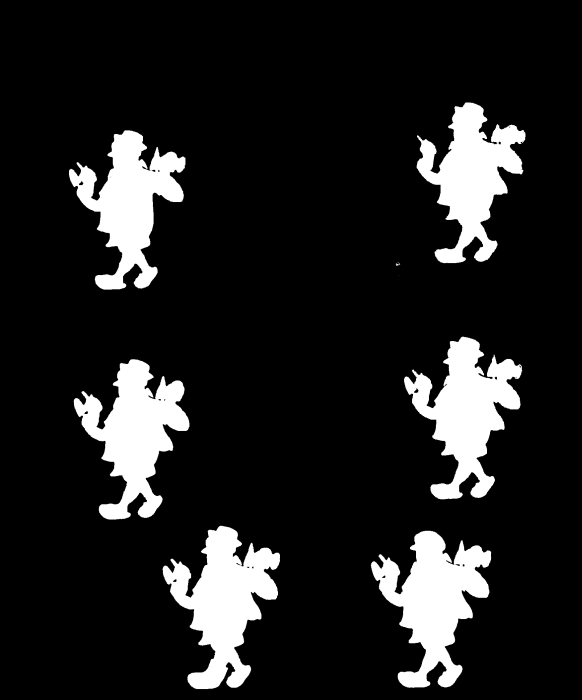
\includegraphics[width=\textwidth]{t3_shadows_mask.png}
        \caption{Purple threshold}
    \end{subfigure}
    \begin{subfigure}{0.4\textwidth}
        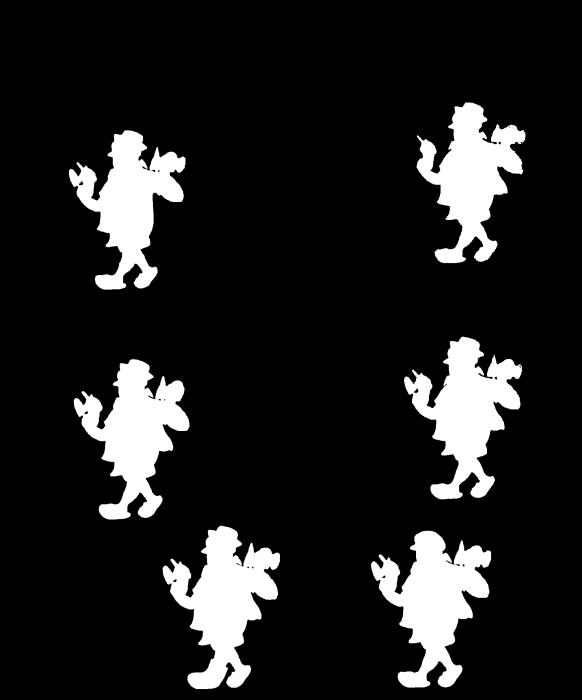
\includegraphics[width=\textwidth]{t3_shadows_kept.png}
        \caption{The six kept blobs}
    \end{subfigure}
    \caption{Finding the silhouettes.}
\end{figure}

%--------------------------------------------------------------
\subsection{Step 2: Finding the man's silhouette}
%--------------------------------------------------------------

The man is made of many colours, so instead of selecting him we select the background and take the man as what is left. The background is a pale, low-saturation green that gets slightly darker towards the edges of the page. The threshold range is hue 15--75, saturation 10--95 and value 140--230. We found it by trying values and checking how well the man's silhouette came out. Only background regions larger than 100\,000 pixels are kept as background. The green shorts, which have almost the same colour as the page, form a smaller island enclosed by the man's dark outline, so they are not removed and stay part of the man.

After the background is removed, the largest remaining blob is the man. The other blobs that remain are the six silhouettes, the circled letters, the title and the icons in the corners, and they are all smaller than the man.

\begin{figure}[H]
    \centering
    \begin{subfigure}{0.24\textwidth}
        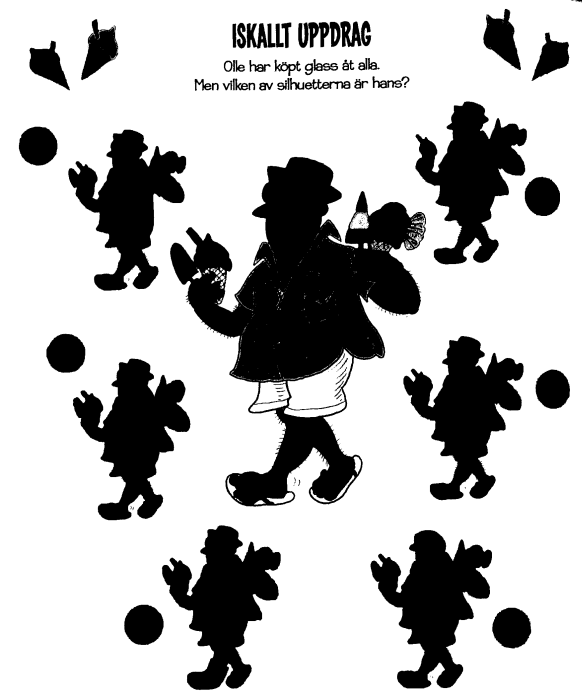
\includegraphics[width=\textwidth]{t3_bg_mask.png}
        \caption{Background threshold}
    \end{subfigure}
    \begin{subfigure}{0.24\textwidth}
        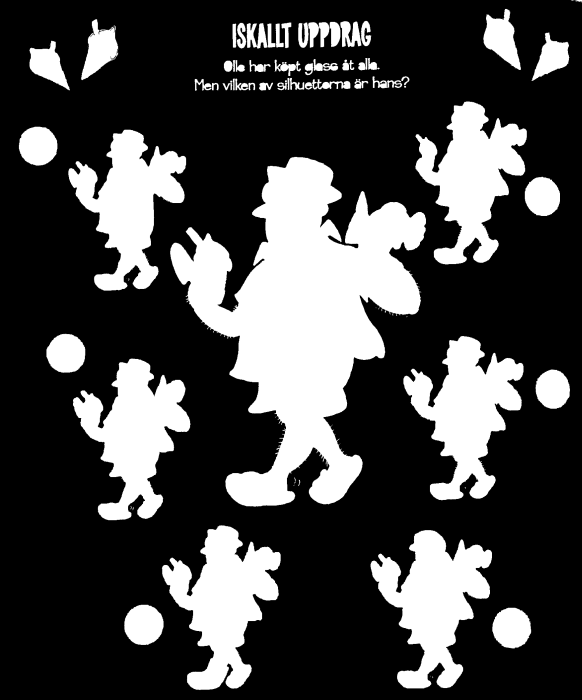
\includegraphics[width=\textwidth]{t3_not_bg.png}
        \caption{Everything that is not background}
    \end{subfigure}
    \begin{subfigure}{0.24\textwidth}
        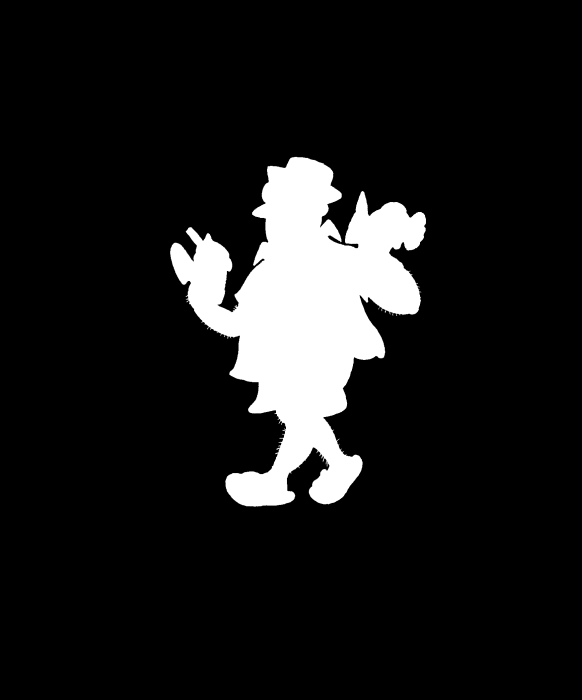
\includegraphics[width=\textwidth]{t3_man.png}
        \caption{Largest blob (the man)}
    \end{subfigure}
    \begin{subfigure}{0.24\textwidth}
        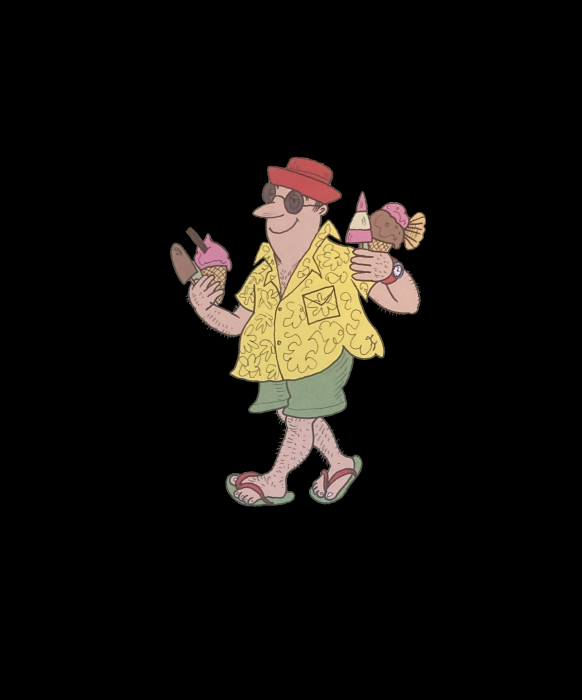
\includegraphics[width=\textwidth]{t3_man_image.png}
        \caption{Applied to the image}
    \end{subfigure}
    \caption{The man's silhouette.}
\end{figure}

%--------------------------------------------------------------
\subsection{Step 3: Comparing the silhouettes with the man}
%--------------------------------------------------------------

The man and the silhouettes have to be compared in the same size and position. Each shape is cropped to its bounding box, scaled so that the longest side is 256 pixels (keeping the proportions, so no shape is stretched), and padded with zeros to a $256\times256$ square.

\paragraph{Mismatch score.} A pixel that belongs to only one of the two shapes is a mismatch. The simplest score, the overlap divided by the union (Jaccard), counts all mismatches equally. This is a problem here. The shapes are aligned only by their bounding boxes, so every edge gets a thin fringe of mismatches, a pixel or two wide, even for a shape that matches. Many such fringes add up to more than one compact patch of real difference, and the best silhouette could be chosen because of the alignment and not because of the shape.

We therefore weight each mismatched pixel by how far it is from the other shape. For every pixel we compute the distance to the nearest pixel of a shape (a distance transform). The cost of a mismatched pixel is the \emph{square} of its distance to the other shape, and the score of a silhouette is the sum of these costs, divided by the area of the man:
\[
    \text{score} = \frac{1}{|M|}\left( \sum_{p \in S\setminus M} d(p, M)^2 + \sum_{p \in M\setminus S} d(p, S)^2 \right),
\]
where $M$ is the man, $S$ is the silhouette and $d(p, X)$ is the distance from pixel $p$ to the nearest pixel of $X$. A pixel just outside the other shape costs almost nothing, so small misalignments are accepted, while a pixel far away costs much more. A lower score means a better match, and the silhouette with the lowest score is the answer. The figure below shows each silhouette (green) on top of the man (red), with yellow where they agree.

\begin{figure}[H]
    \centering
    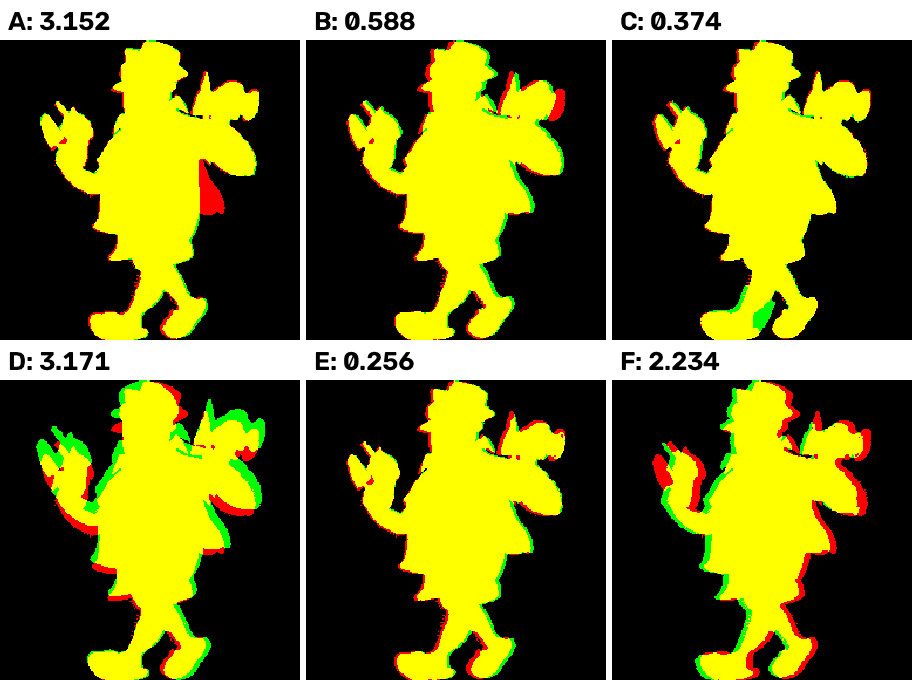
\includegraphics[width=0.7\textwidth]{t3_overlays.png}
    \caption{Mismatch score of each silhouette against the man (lower is better).}
\end{figure}

%--------------------------------------------------------------
\subsection{Result}
%--------------------------------------------------------------

\begin{center}
\begin{tabular}{lc}
\toprule
Silhouette & Mismatch score \\
\midrule
\textbf{E} & \textbf{0.256} \\
C & 0.374 \\
B & 0.588 \\
F & 2.234 \\
A & 3.152 \\
D & 3.171 \\
\bottomrule
\end{tabular}
\end{center}

\textbf{Silhouette E} has the lowest score and is the shadow of the man. Silhouettes F, A and D are clearly worse, with scores about ten times higher, because parts of them are many pixels away from the man's silhouette. The two closest competitors are C and B. Silhouette C has the highest plain overlap with the man (0.939 against 0.911 for E), but one patch of it, near the left foot, lies about eight pixels from the man's silhouette. The squared distance makes this patch cost more than all the thin edge fringes of E, which are at most about four pixels away. The score of E is about 30\,\% lower than that of C.

%--------------------------------------------------------------
\subsection{The second image}
%--------------------------------------------------------------

We also tried the same method on the second image, where the background is a patterned fabric with ovals in many colours. It does not work there. The silhouettes are still found correctly in step 1, since their purple colour is the same, but the man's silhouette in step 2 is wrong: it is merged with parts of the background, and all six silhouettes get a very large and almost equal mismatch score (about 850--920, against 0.3--3.2 on the first image), so no silhouette can be picked.

Figure~\ref{fig:img2man} shows the result of step 2 on the second image, and Figure~\ref{fig:img2overlay} shows how the silhouettes are then compared with this wrong shape.

\begin{figure}[H]
    \centering
    \begin{subfigure}{0.24\textwidth}
        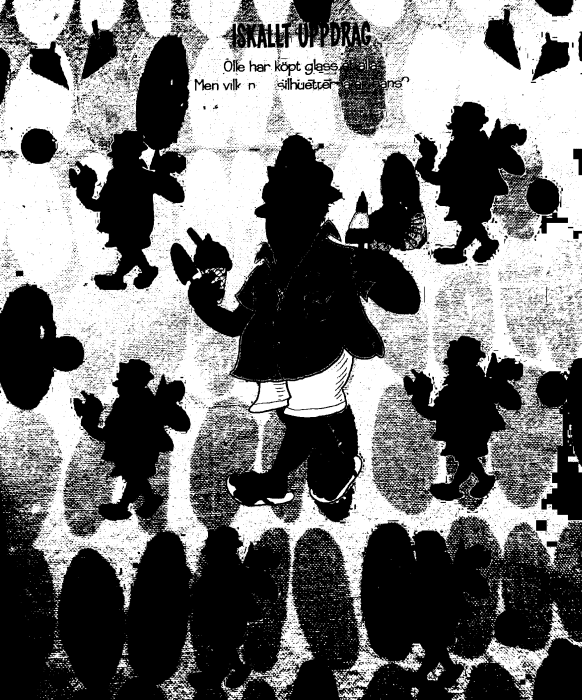
\includegraphics[width=\textwidth]{t3b_bg_mask.png}
        \caption{Background threshold}
    \end{subfigure}
    \begin{subfigure}{0.24\textwidth}
        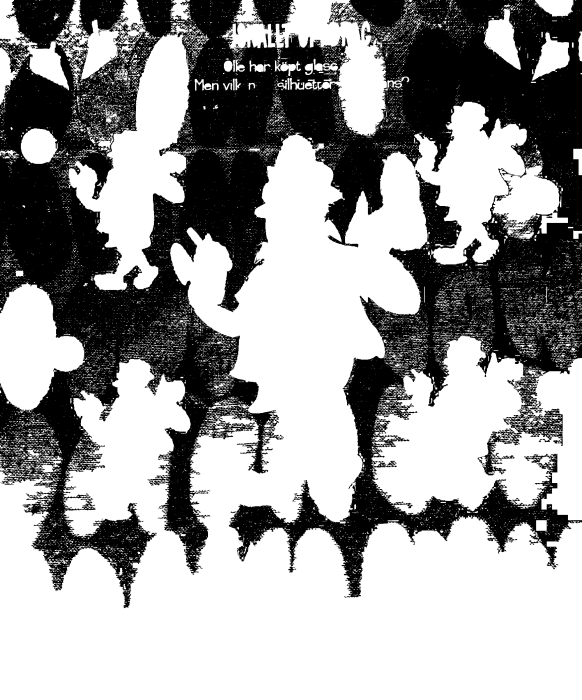
\includegraphics[width=\textwidth]{t3b_not_bg.png}
        \caption{Everything that is not background}
    \end{subfigure}
    \begin{subfigure}{0.24\textwidth}
        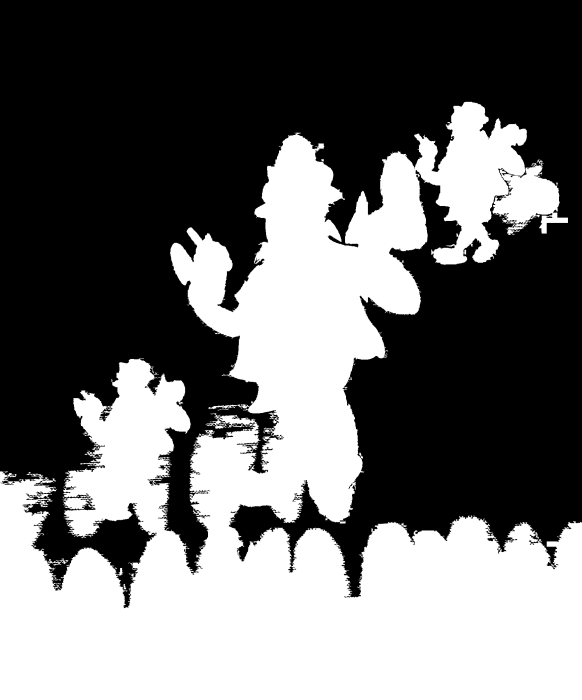
\includegraphics[width=\textwidth]{t3b_man.png}
        \caption{Largest blob}
    \end{subfigure}
    \begin{subfigure}{0.24\textwidth}
        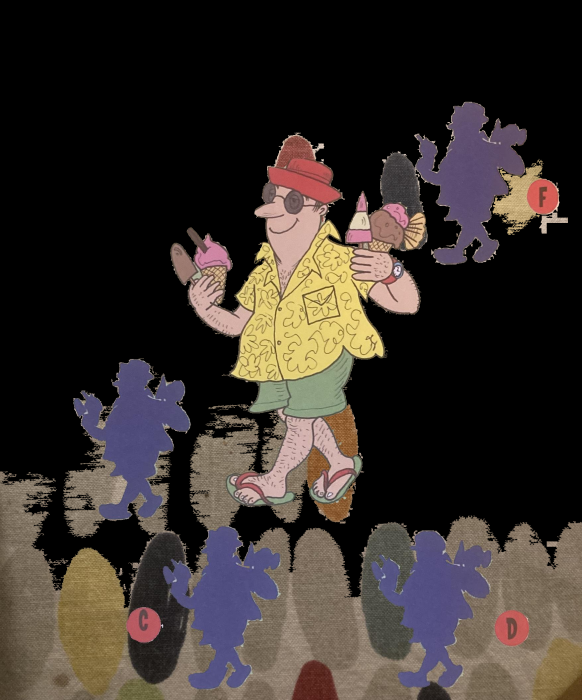
\includegraphics[width=\textwidth]{t3b_man_image.png}
        \caption{Applied to the image}
    \end{subfigure}
    \caption{Step 2 on the second image. The background threshold removes only part of the fabric, so the largest blob contains the man together with the fabric at the bottom of the image, the ovals behind him and the silhouettes next to them.}
    \label{fig:img2man}
\end{figure}

\begin{figure}[H]
    \centering
    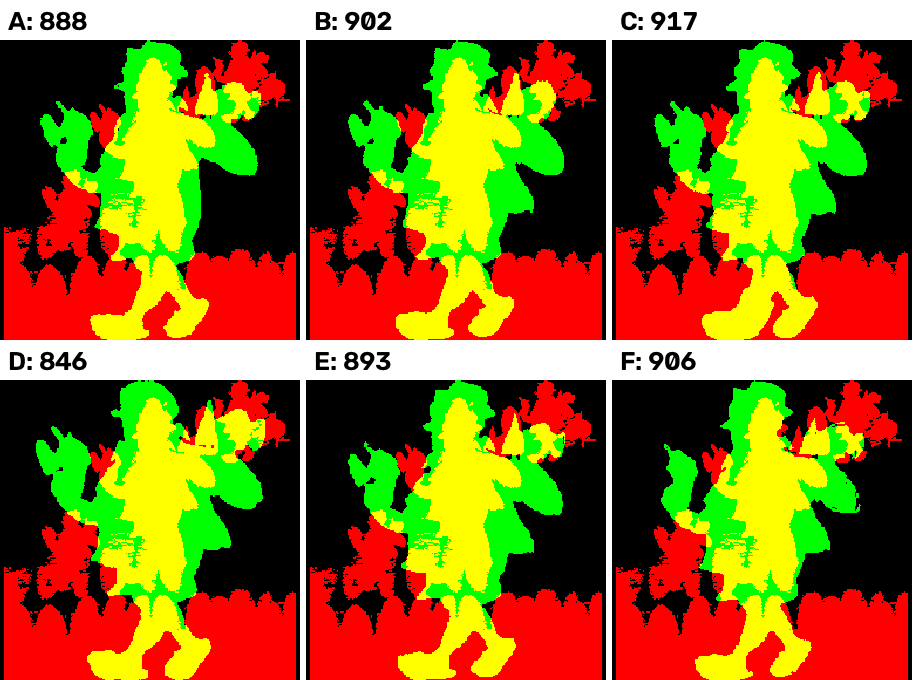
\includegraphics[width=0.7\textwidth]{t3b_overlays.png}
    \caption{Second image: each silhouette (green) on top of the man's wrong silhouette (red), with the mismatch score. All scores are large and similar, so none of them says anything about the shapes.}
    \label{fig:img2overlay}
\end{figure}

The reason is that the background has no single colour range. The fabric and its ovals cover the same values of hue, saturation and brightness as the man's skin, clothes and hat, so a colour threshold that removes the fabric also removes parts of the man, and a threshold that keeps the man also keeps parts of the fabric. Adjusting the range to fit both images, and shrinking the image to average out the grain of the fabric, improved the mask but never made it clean.

%--------------------------------------------------------------
\subsection{A method that does not use the man}
%--------------------------------------------------------------

The difficulty on the second image comes entirely from segmenting the man. The six silhouettes, on the other hand, are found correctly in both images, because their purple colour is the same. This suggests a way to find the answer without the man: if the five wrong silhouettes are variations of the true one, each differing from it in a different place, then the true silhouette should be the one closest to the \emph{average} of all six. This is implemented in a separate script, and the steps are:
\begin{enumerate}
    \item Find the six silhouettes as in step 1.
    \item Scale each of them to the same $256\times256$ square as in step 3.
    \item Compute the average of the six squares pixel by pixel. The result is a grey-level image: white where all six silhouettes are filled, black where none is, and grey where only some of them are.
    \item Threshold the average at one half. This gives a \emph{typical shape}: the pixels that are filled in at least half of the silhouettes.
    \item Compare each silhouette with the typical shape using the mismatch score of step 3. The lowest score is the answer.
\end{enumerate}

The background is never used, so the fabric of the second image does not matter.

\begin{figure}[H]
    \centering
    \begin{subfigure}{0.27\textwidth}
        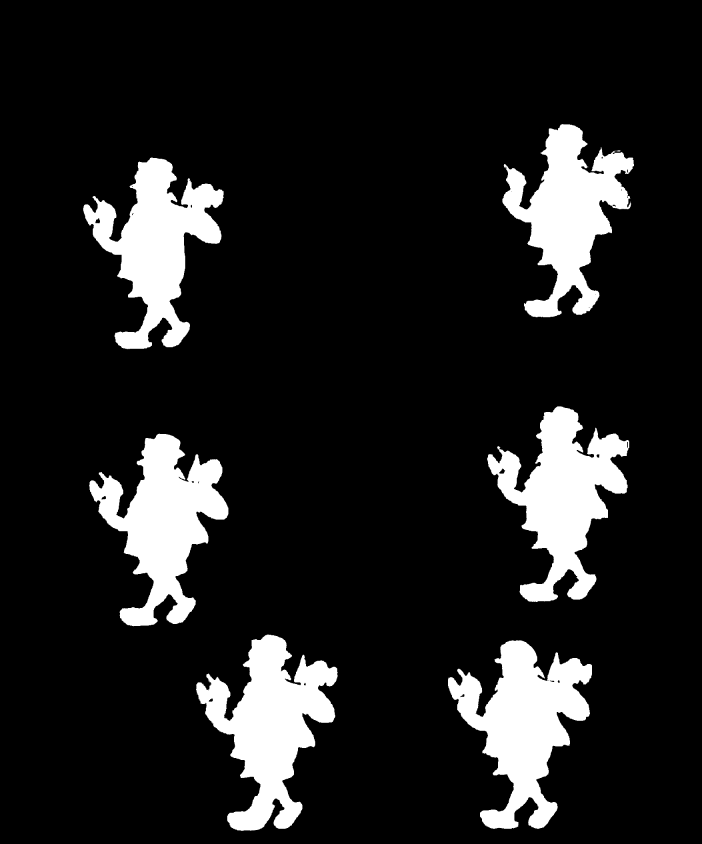
\includegraphics[width=\textwidth]{t3c_kept.png}
        \caption{The six silhouettes}
    \end{subfigure}
    \begin{subfigure}{0.27\textwidth}
        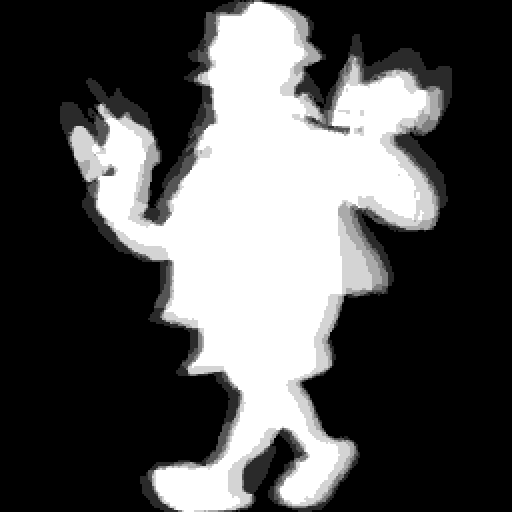
\includegraphics[width=\textwidth]{t3c_average.png}
        \caption{Average of the six}
    \end{subfigure}
    \begin{subfigure}{0.27\textwidth}
        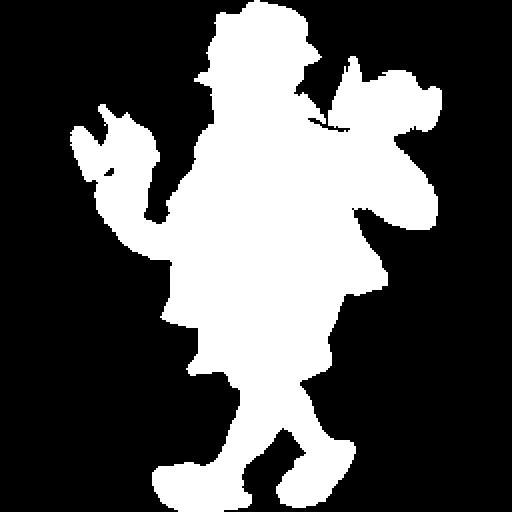
\includegraphics[width=\textwidth]{t3c_typical.png}
        \caption{Typical shape (threshold 0.5)}
    \end{subfigure}
    \caption{Second image: from the silhouettes to the typical shape.}
\end{figure}

\begin{figure}[H]
    \centering
    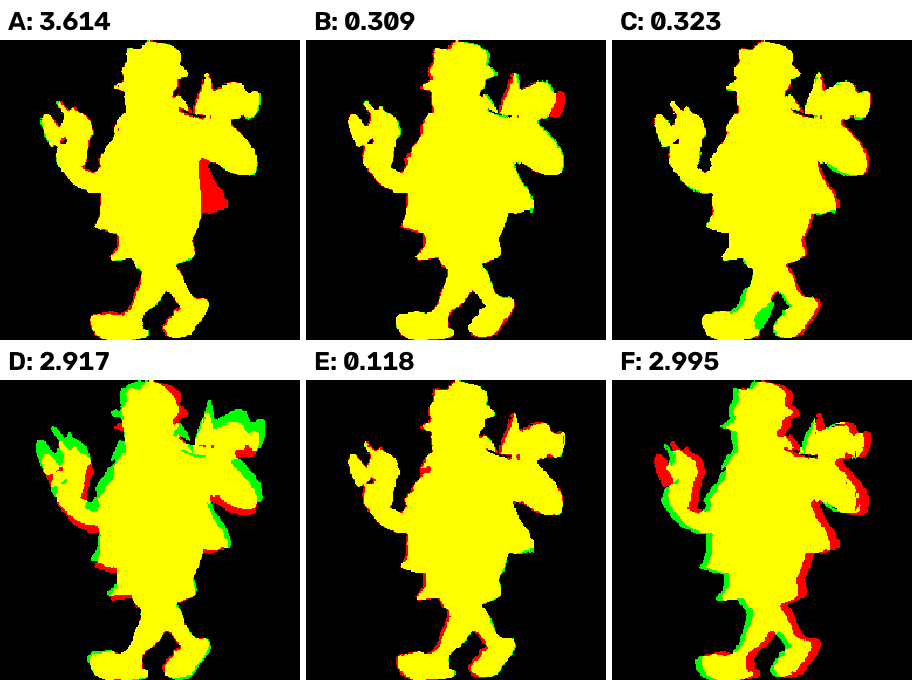
\includegraphics[width=0.6\textwidth]{t3c_overlays.png}
    \caption{Second image: each silhouette (green) on top of the typical shape (red), with the mismatch score (lower is better).}
\end{figure}

\begin{center}
\begin{tabular}{lc}
\toprule
Silhouette & Mismatch score \\
\midrule
\textbf{E} & \textbf{0.118} \\
B & 0.309 \\
C & 0.323 \\
D & 2.917 \\
F & 2.995 \\
A & 3.614 \\
\bottomrule
\end{tabular}
\end{center}

\textbf{Silhouette E} has the lowest score on the second image, which is the same answer as the method with the man gave on the first image. Its score is less than 40\,\% of that of the next silhouettes (B and C), and D, F and A are about ten times worse than E. Running the same script on the first image also gives E (score 0.075, against 0.326 for the second best).

The method assumes that the wrong silhouettes are scattered around the true one, so it fails if they are all changed in the same way. It also never compares the silhouette with the man, so it is a second, independent piece of evidence and not a proof that E is the man's shadow.

%==============================================================
\section{Task 4: Convolutional neural network}
%==============================================================

The network takes a $32\times32$ grayscale image and has the following layers.

\begin{center}
\begin{tabular}{lll}
\toprule
Layer & Output size & Parameters \\
\midrule
Input & $32\times32\times1$ & \\
Convolution, $3\times3$, 16 channels, stride 1, padding 1 & $32\times32\times16$ & 160 \\
ReLU & $32\times32\times16$ & 0 \\
Max pooling, $4\times4$, stride 4 & $8\times8\times16$ & 0 \\
Convolution, $3\times3$, 32 channels, stride 1, padding 1 & $8\times8\times32$ & 4\,640 \\
ReLU & $8\times8\times32$ & 0 \\
Max pooling, $2\times2$, stride 2 & $4\times4\times32$ & 0 \\
Fully connected, $512 \to 5$ & $5$ & 2\,565 \\
Softmax & $5$ & 0 \\
\midrule
Total & & \textbf{7\,365} \\
\bottomrule
\end{tabular}
\end{center}

\subsection*{a) Number of parameters}

A convolutional layer with a $k\times k$ kernel, $c_\text{in}$ input channels and $c_\text{out}$ output channels has $k^2\, c_\text{in}\, c_\text{out}$ weights and $c_\text{out}$ biases. The ReLU, max-pooling and softmax layers have no trainable parameters.

\paragraph{Convolution 1} (3$\times$3 kernel, 1 input channel because the image is grayscale, 16 output channels):
\[
    3\cdot 3\cdot 1\cdot 16 + 16 = 144 + 16 = 160 .
\]

\paragraph{Convolution 2} (3$\times$3 kernel, 16 input channels, 32 output channels):
\[
    3\cdot 3\cdot 16\cdot 32 + 32 = 4608 + 32 = 4640 .
\]

\paragraph{Fully connected layer} ($4\cdot4\cdot32 = 512$ input nodes, 5 output nodes):
\[
    512\cdot 5 + 5 = 2560 + 5 = 2565 .
\]

The total number of parameters that have to be found and stored is
\[
    160 + 4640 + 2565 = \boxed{7365} .
\]

As a check of the layer sizes: the padding of 1 keeps the $3\times3$ convolutions at the same size, so $32\to32$. The $4\times4$ pooling with stride 4 gives $32/4 = 8$, and the $2\times2$ pooling with stride 2 gives $8/2 = 4$. This gives $4\times4\times32 = 512$ values, which is the input size of the fully connected layer.

\begin{figure}[H]
    \centering
    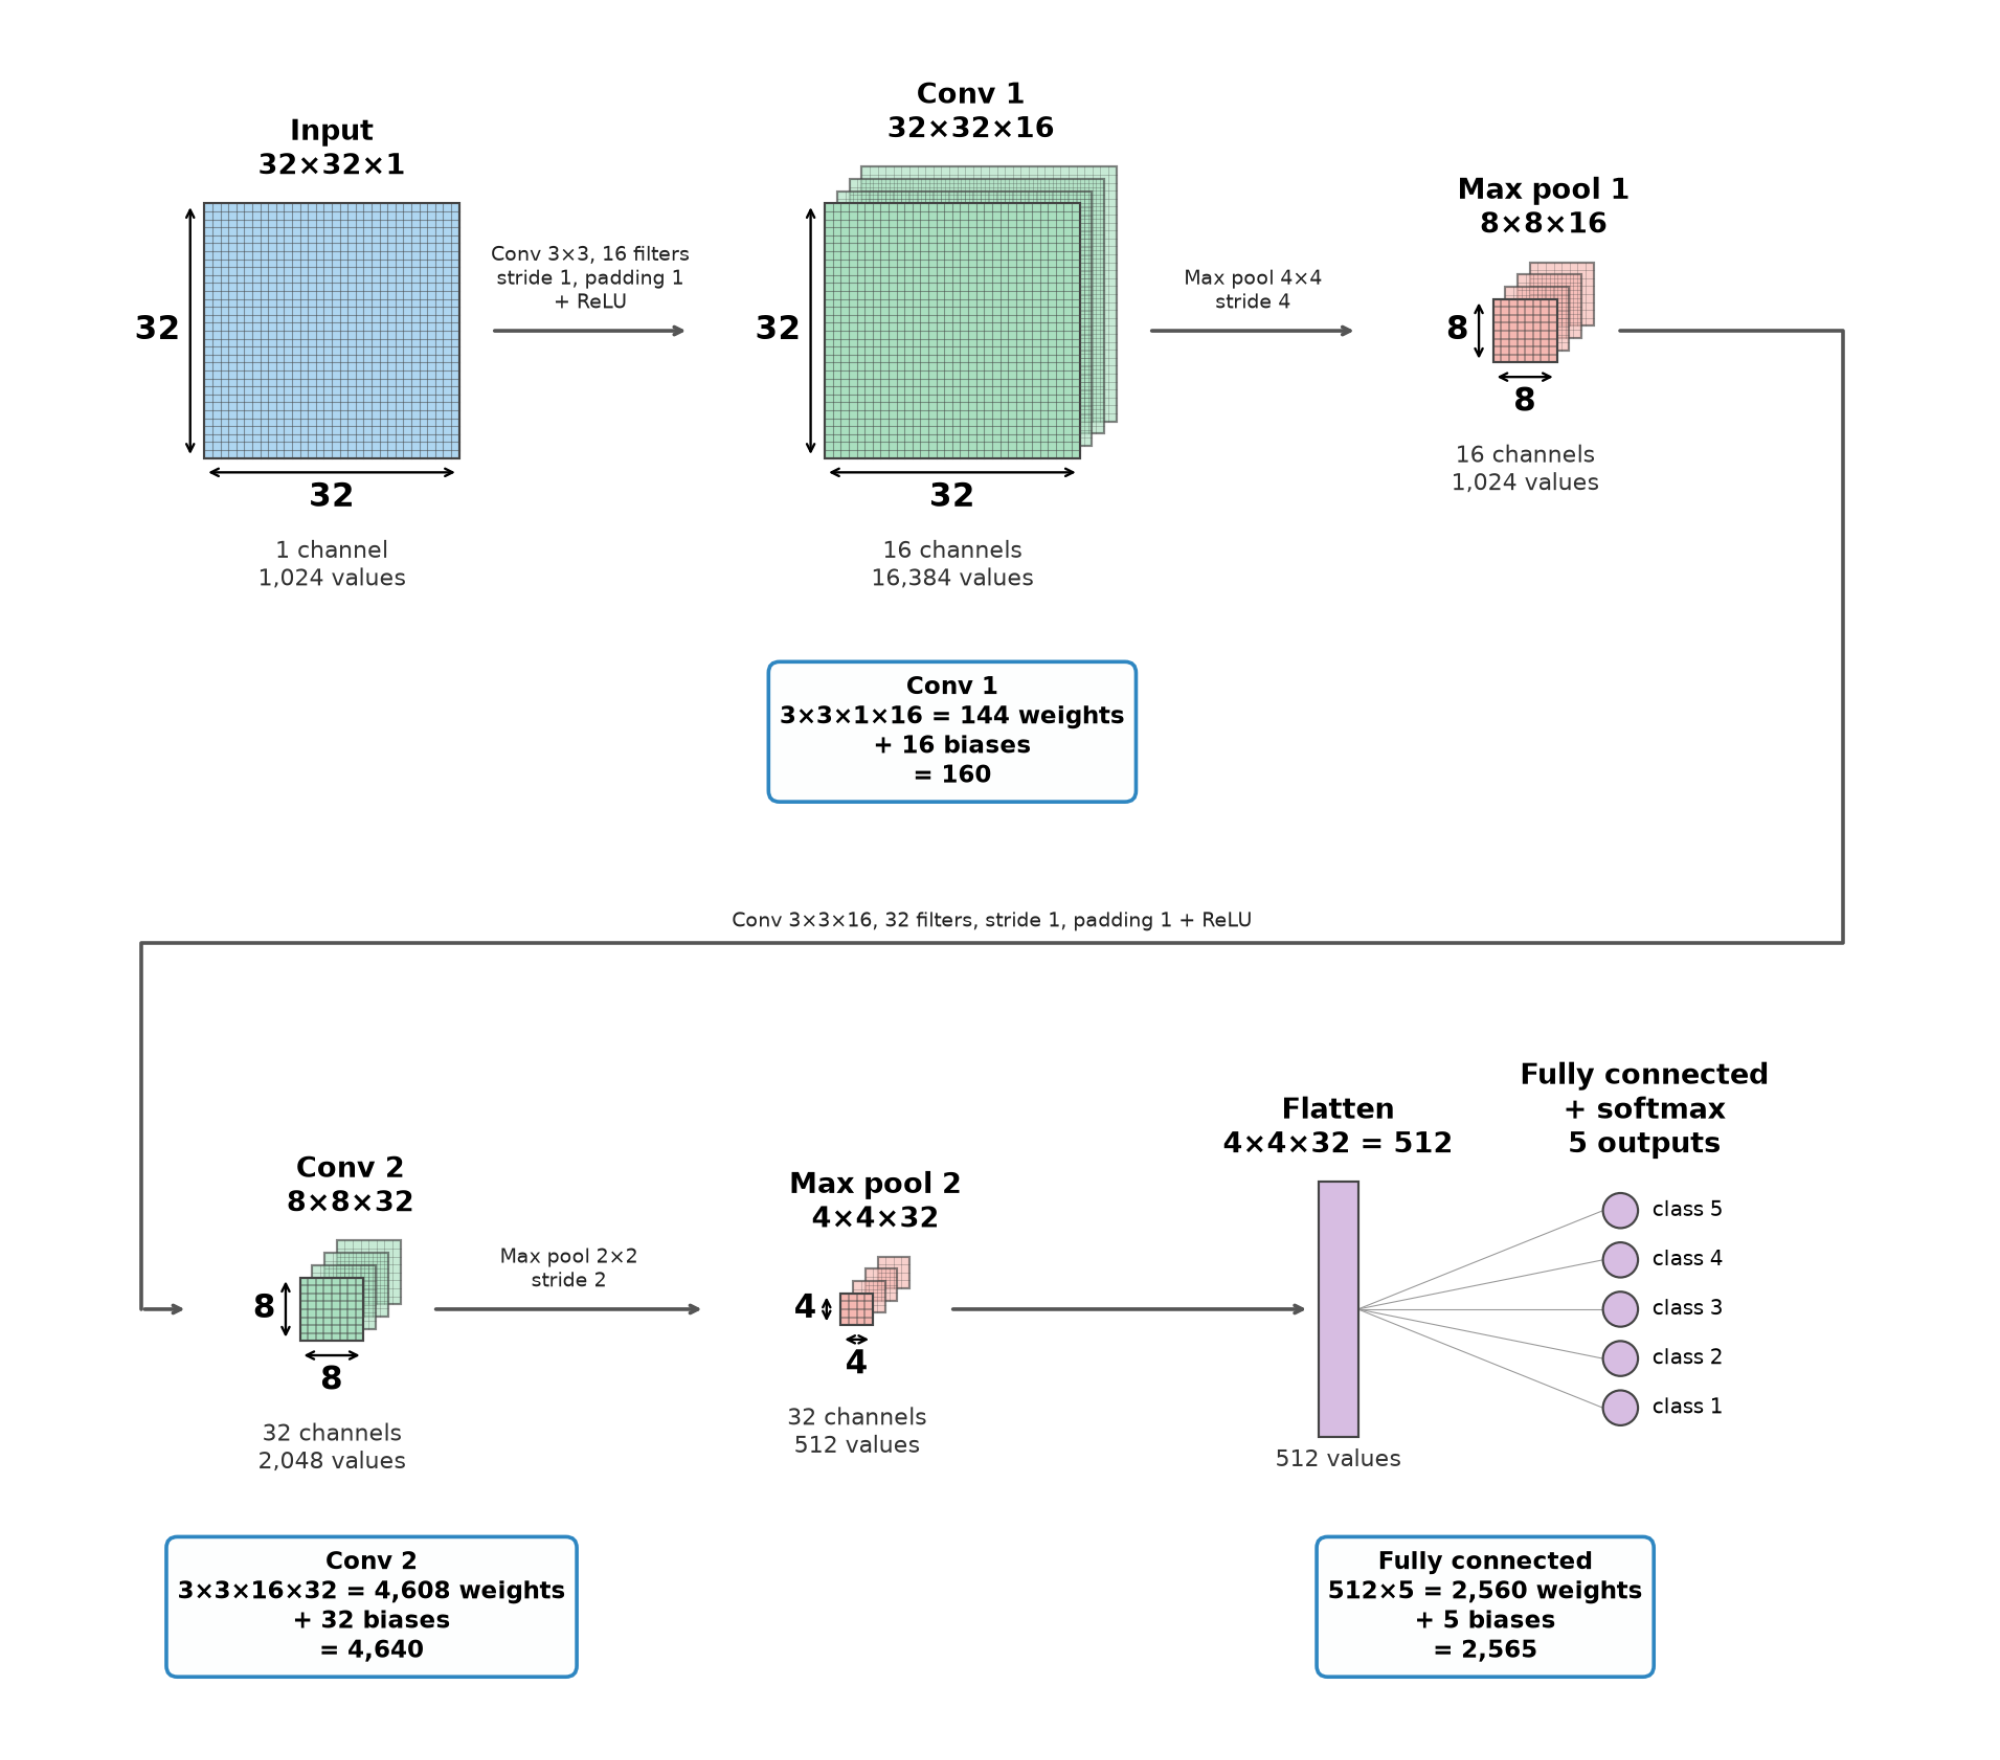
\includegraphics[width=\textwidth]{t4_parameters.png}
    \caption{The feature maps at their real size (one cell is one value) and the parameters of each layer. ReLU, max pooling and softmax have no parameters.}
\end{figure}

\subsection*{b) Receptive field of the final max-pooling layer}

The receptive field of a feature in a given layer is the region of the original input image that influences that feature. It is computed by tracing backwards through the network, layer by layer. Since all kernels are symmetric, it is enough to reason in one dimension. ReLU works on each value separately and does not change the receptive field.

\paragraph{Max pooling 2} ($2\times2$, stride 2). One output feature looks at a $2\times2$ block in the output of convolution 2.

\paragraph{Convolution 2} ($3\times3$, stride 1). A $3\times3$ kernel sliding over a $2\times2$ block covers a $4\times4$ region in the output of max pooling 1, because the kernel extends 1 pixel beyond each edge of the block: $2 + 1 + 1 = 4$.

\paragraph{Max pooling 1} ($4\times4$, stride 4). Each value in the output of max pooling 1 corresponds to a $4\times4$ block in the output of convolution 1. A $4\times4$ region in the output of max pooling 1 therefore covers $4\cdot4 = 16$ values in each direction, a $16\times16$ region, in the output of convolution 1.

\paragraph{Convolution 1} ($3\times3$, stride 1). A $3\times3$ kernel sliding over a $16\times16$ block covers a region of $16 + 1 + 1 = 18$ pixels in each direction of the original input.

The receptive field of the features in the final max-pooling layer is therefore
\[
    \boxed{18\times18} .
\]
This means that each output value of max pooling 2 is influenced by an $18\times18$ patch of the original $32\times32$ input image.

\begin{figure}[H]
    \centering
    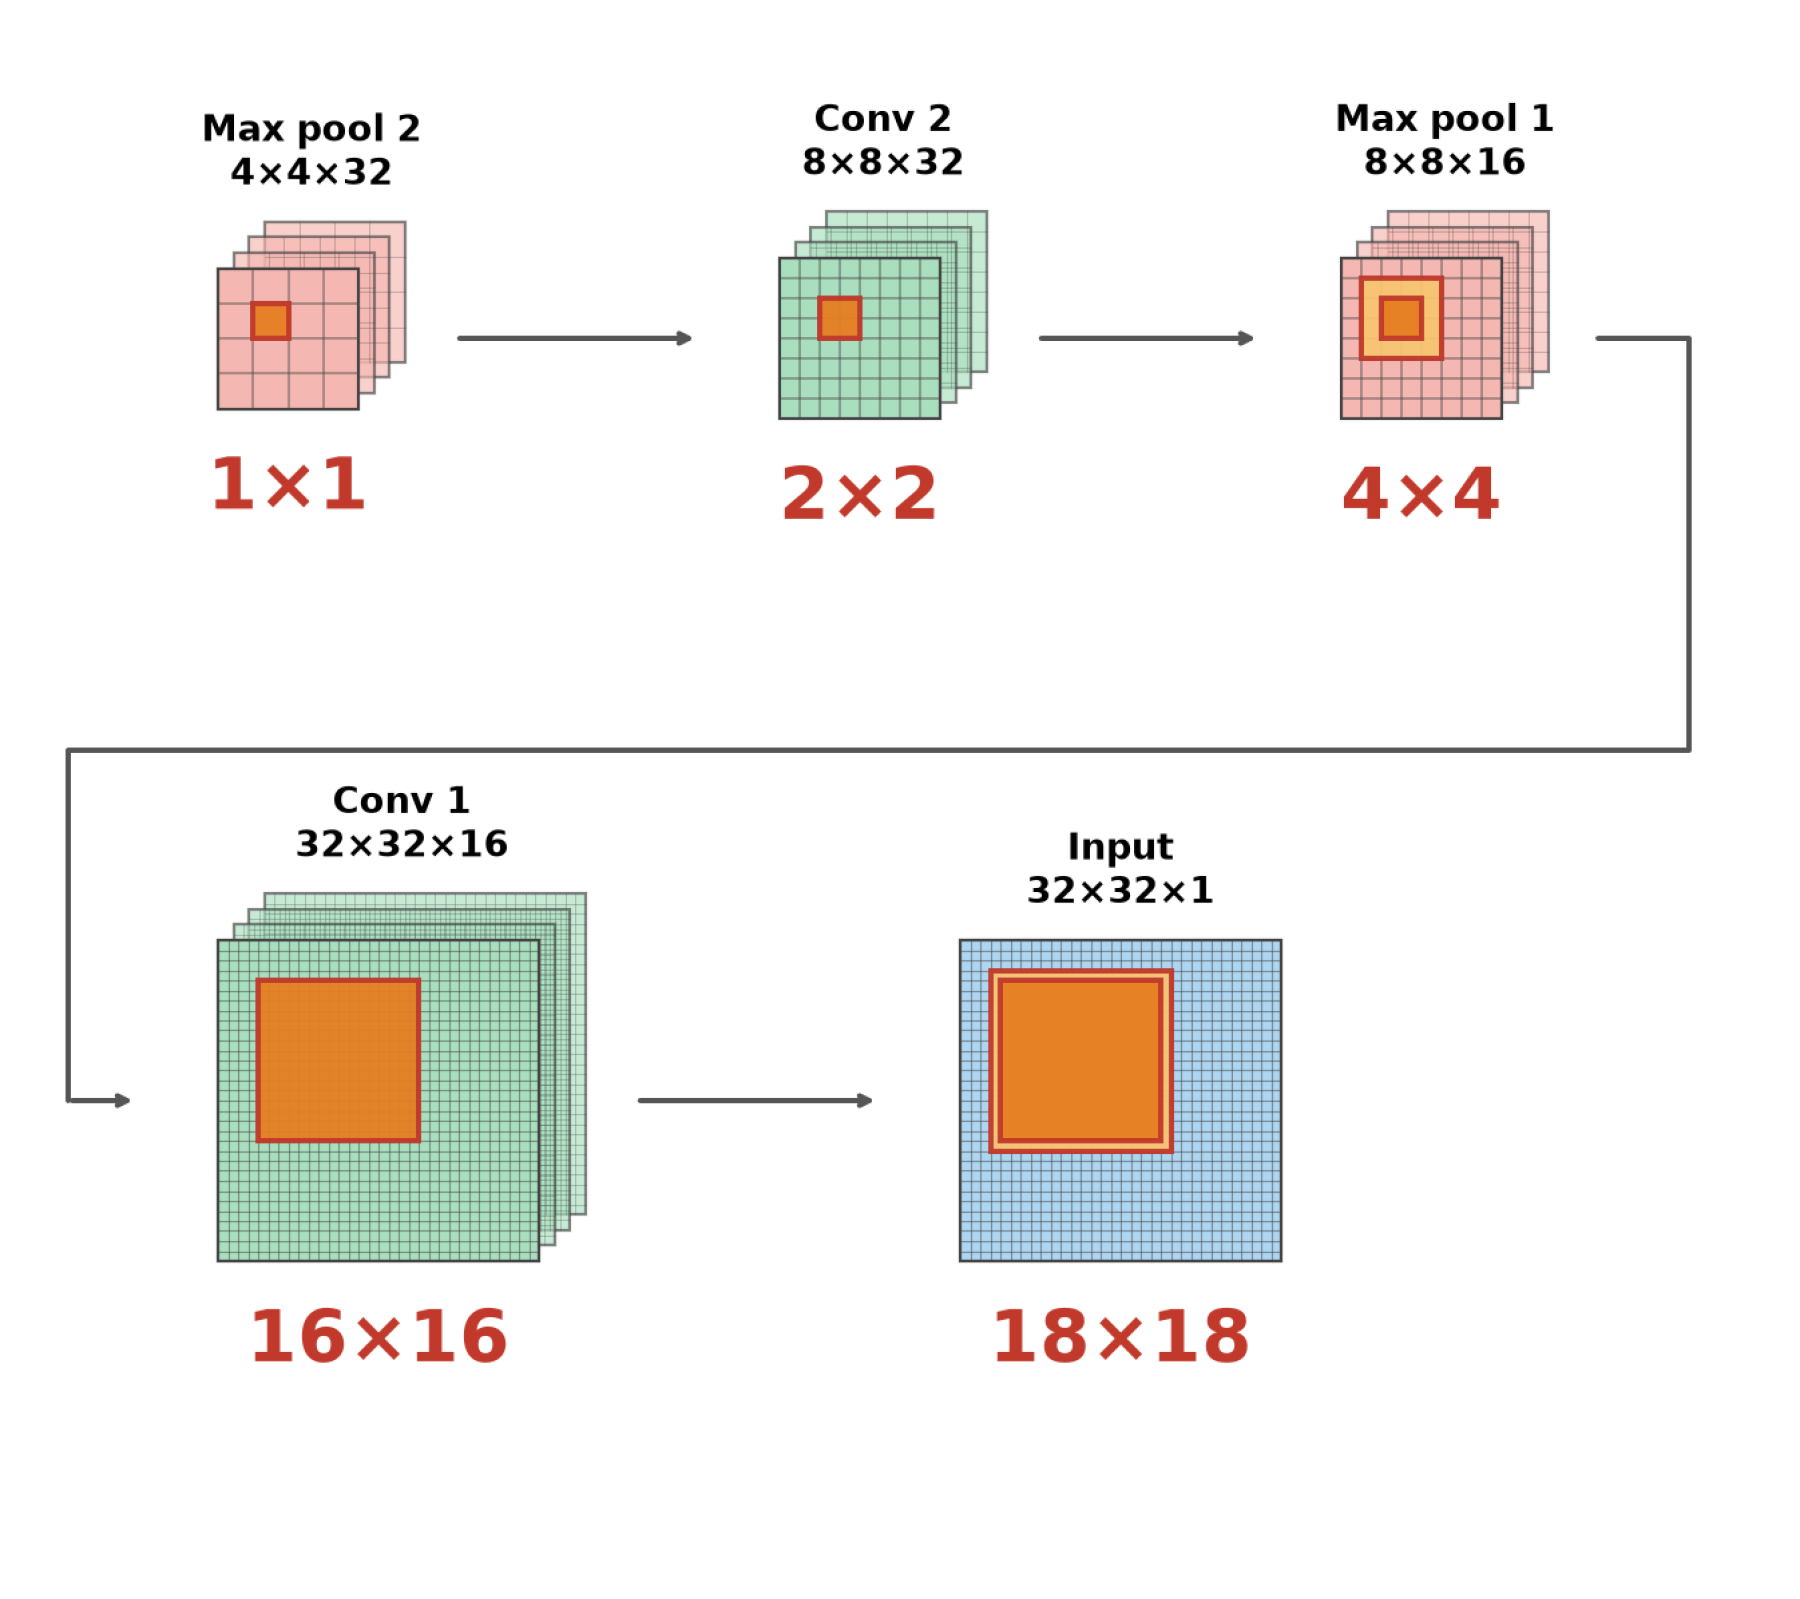
\includegraphics[width=0.8\textwidth]{t4_receptive_field.png}
    \caption{The four steps of b), from the last max-pooling layer back to the input. The orange cells are the values that one feature of max pooling 2 depends on, and the size of each region is written under the layer. The light orange ring is the pixel added on each side by a $3\times3$ convolution. The small maps are drawn with larger cells than the large ones, so that the marked cells can be seen.}
\end{figure}

%==============================================================
\section{Task 5: Finding the missing red channel}
%==============================================================

Two images of the same scene with toy cars are given. The first is complete. In the second, taken from a different position, the red channel is zero, so only green and blue are available, and the task is to estimate the red channel of the second image automatically. The colour of an object does not depend on where it is in the image: a red car is red in both images. So the relation between the green and blue values of a pixel and its red value can be learned from image 1 and applied to image 2. Every pixel of image 1 is a training example, with $(G, B)$ as input and the known $R$ as the answer. We tried three methods, linear regression, RANSAC and k nearest neighbours. The red channel from k-NN was noisy, so we added a noise reduction step and tried two filters, a Gaussian filter and anisotropic diffusion. Finally we averaged the red channels of linear regression and the denoised k-NN.

\begin{figure}[H]
    \centering
    \begin{subfigure}{0.32\textwidth}
        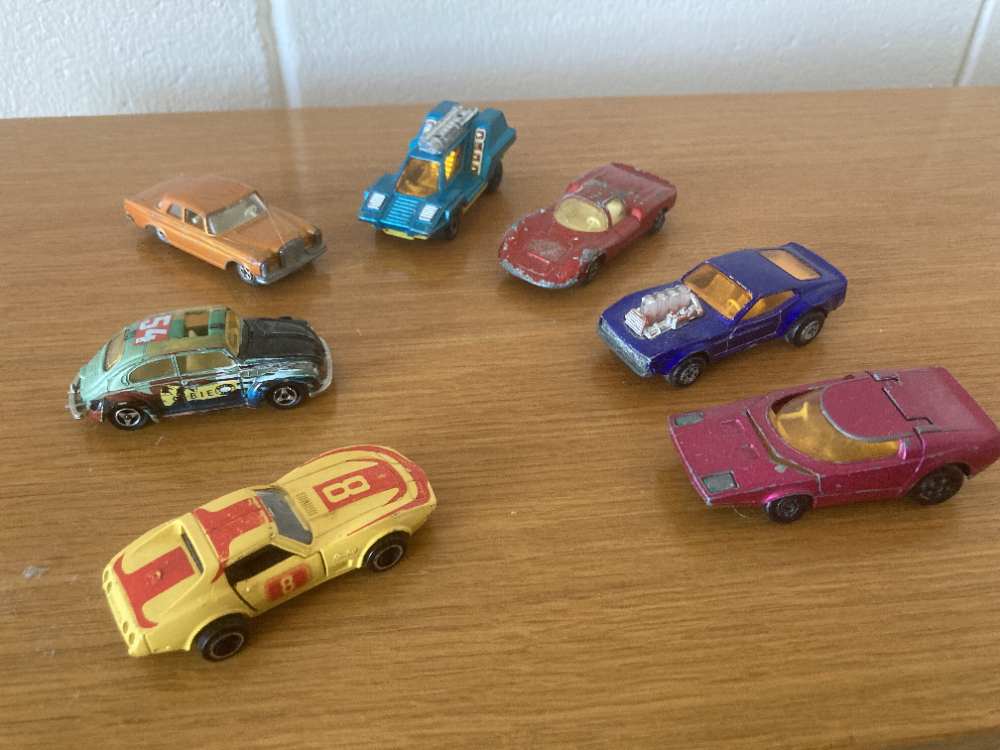
\includegraphics[width=\textwidth]{t5_image1.png}
        \caption{Image 1: complete}
    \end{subfigure}
    \begin{subfigure}{0.32\textwidth}
        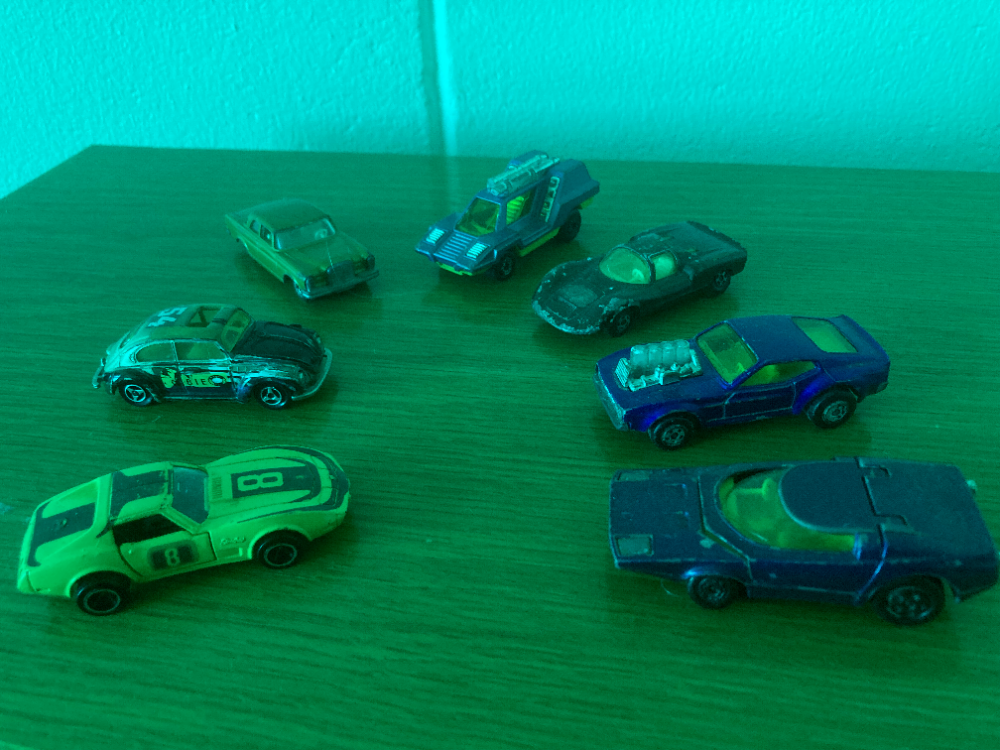
\includegraphics[width=\textwidth]{t5_image2_given.png}
        \caption{Image 2: no red channel}
    \end{subfigure}
    \caption{The two input images.}
\end{figure}

The red channel of image 2 is not known, so we cannot measure the methods on it. Image 1 has a known red channel, and we use it to measure how well a method predicts the red channel of pixels it has not learned from. We cut image 1 into squares of $42\times42$ pixels, 24 across and 18 down, and divided them into six equally large groups with a regular pattern: the square in column $x$ and row $y$ goes to group $(x + 2y) \bmod 6$. Group 0 is the test set and groups 1 to 5 are five folds. Every group has 72 squares spread evenly over the image, and every row of squares contains all six groups, so each group contains the same kinds of squares (wall, table, dark cars, red cars).

The test set is never used for learning or for choosing settings. It is used once, at the end, to compare the methods. The folds are used for 5-fold cross-validation to choose the settings of each method. In each of the 5 rounds one fold is the validation fold: the method learns from the other four folds, predicts the red channel of the validation fold from its green and blue values, and is compared with the true red channel there. After the 5 rounds every pixel outside the test set has been predicted by a model that did not see it, and the errors are computed over all these pixels. The setting with the smallest error is chosen. In the figure, the test squares are pink in the first picture and black in the five rounds, since they are not used at all. In each round the validation fold is pink and the other squares are the ones the method learns from. We measure the error with the RMSE, the root of the mean squared error of the red channel in grey levels (0--255). It punishes large errors strongly, and lower is better.

\begin{figure}[H]
    \centering
    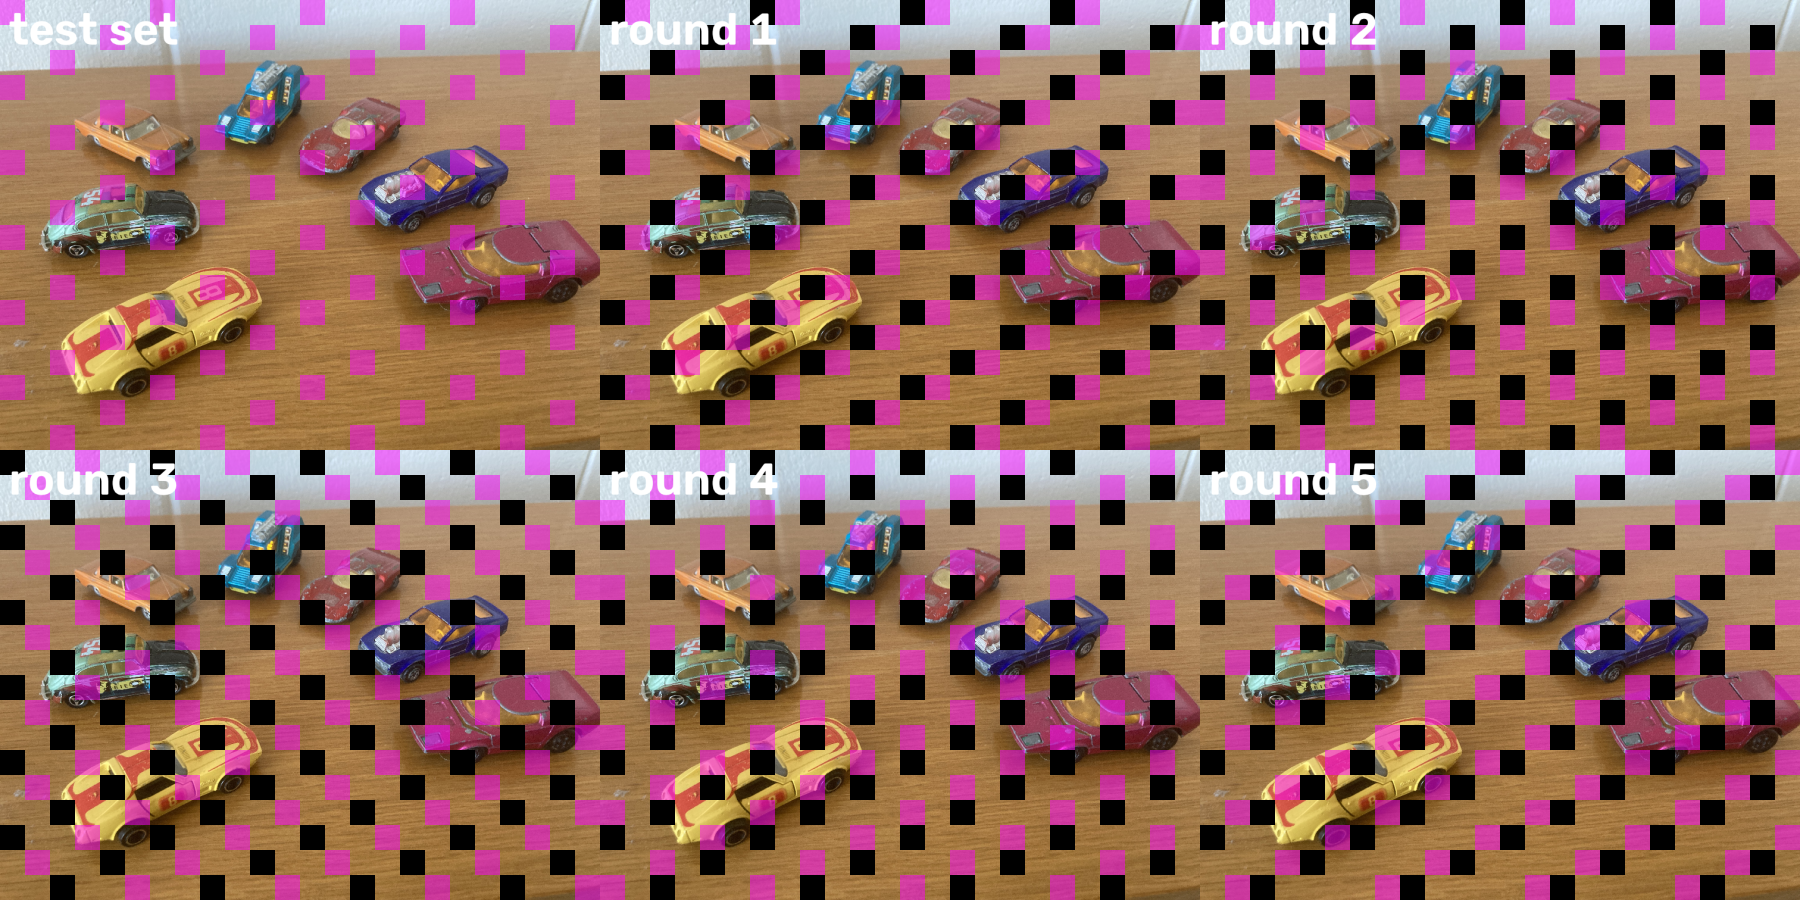
\includegraphics[width=0.92\textwidth]{t5_splits.png}
    \caption{First picture: the test set (pink). Rounds 1 to 5 of the cross-validation: the test squares are black (not used), the validation fold is pink, and the other squares are used for learning.}
\end{figure}

Linear regression assumes that the red value is a linear combination of the green and blue values, $R \approx a\,G + b\,B + c$, and finds $a$, $b$ and $c$ with least squares on all pixels of image 1. The result is $R = 1.13\,G - 0.41\,B + 52.3$. For image 2 we compute $\hat R$ from its green and blue values and clip it to $[0, 255]$. It has no setting to choose, and its cross-validation error is RMSE 17.33.

The linear model is pulled away from the majority of the pixels by the pixels where green and blue say little about red, for example the red cars. RANSAC fits the same model but ignores such pixels. Three random pixels define a candidate plane for $R$, a pixel is an inlier if its red value is within a threshold of the plane, and the plane with the most inliers out of 500 attempts is kept. The final parameters are a least squares fit to the inliers only. We chose the threshold with cross-validation:

\begin{center}
\begin{tabular}{lccccc}
\toprule
Threshold & 5 & 10 & 20 & 40 & \textbf{80} \\
\midrule
RMSE & 21.13 & 21.62 & 18.13 & 17.43 & \textbf{17.32} \\
\bottomrule
\end{tabular}
\end{center}

With a small threshold RANSAC only fits the pixels that follow one plane closely, and the pixels that do not follow it get large errors, so the RMSE is large. When the threshold grows, RANSAC includes more and more pixels and becomes the ordinary linear regression. The smallest RMSE is at the largest threshold we tried, 80, where the result is practically the same as linear regression (17.32 against 17.33), so for this data RANSAC does not improve on the linear model, and we used 80.

A linear model cannot represent that very different reds share a similar $(G, B)$, so we also tried k nearest neighbours, which makes no assumption about the form of the relation. For a pixel of image 2 it finds the $k$ pixels of image 1 with the most similar $(G, B)$ and averages their red values with weights $1/d^2$, where $d$ is the distance in $(G, B)$.  We tried $k$ from 5 to 800 with cross-validation:

\begin{center}
\begin{tabular}{lcccccccc}
\toprule
$k$ & 5 & 10 & 25 & 50 & \textbf{100} & 200 & 400 & 800 \\
\midrule
RMSE & 14.11 & 13.91 & 13.84 & \textbf{13.82} & \textbf{13.82} & 13.83 & 13.85 & 13.92 \\
\bottomrule
\end{tabular}
\end{center}

The error is almost the same for $k = 50$, 100 and 200 and the curve is flat from $k = 25$ to $k = 400$ (RMSE 13.82--13.85), so the choice of $k$ is not sensitive. We used $k = 100$, in the middle of the flat part. The figure shows image 2 with the red channel from the three methods. Linear regression and RANSAC turn the red car dark brown and the pink car dark purple. k-NN gives the red stripes on the yellow car and the pink car a red colour, but it leaves the red car brown. It also gives the wall a cyan tint: the green and blue values of the wall in image 2 are not the same as in image 1, so the neighbours that k-NN finds are not wall pixels.

\begin{figure}[H]
    \centering
    \begin{subfigure}{0.32\textwidth}
        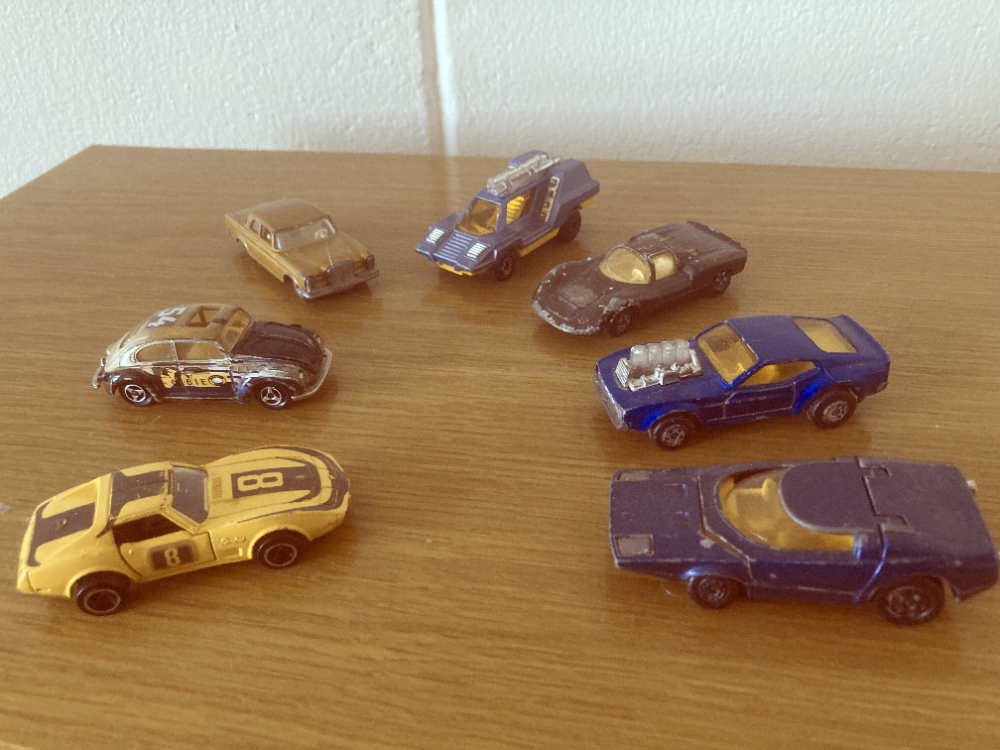
\includegraphics[width=\textwidth]{t5_linear.png}
        \caption{Linear regression}
    \end{subfigure}
    \begin{subfigure}{0.32\textwidth}
        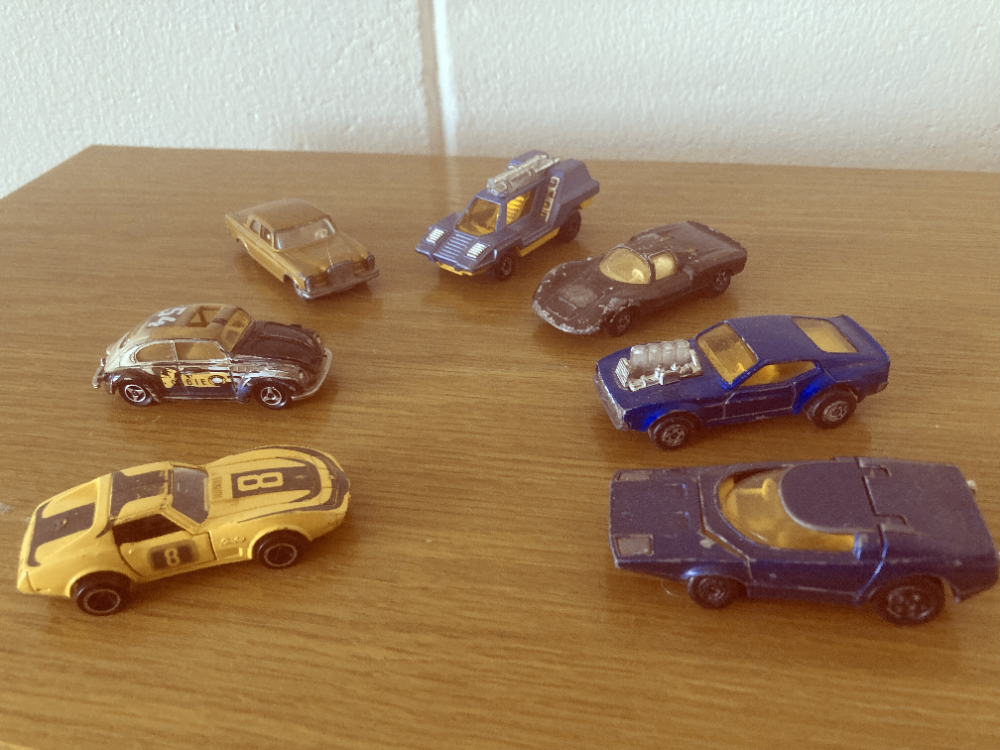
\includegraphics[width=\textwidth]{t5_ransac.png}
        \caption{RANSAC}
    \end{subfigure}
    \begin{subfigure}{0.32\textwidth}
        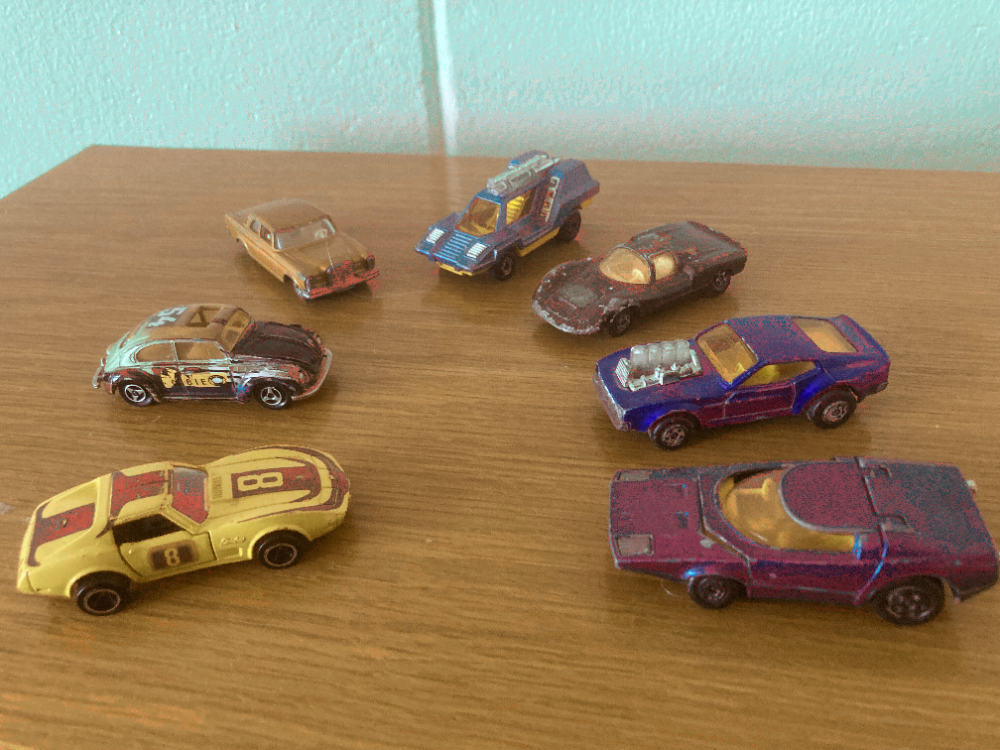
\includegraphics[width=\textwidth]{t5_knn.png}
        \caption{k nearest neighbours}
    \end{subfigure}
    \caption{Image 2 with the red channel estimated by the three methods. RANSAC with threshold 80 looks the same as linear regression.}
\end{figure}

The red channel from k-NN is noisy: pixels with almost the same green and blue values can get quite different red values, which gives a grainy texture, as the zoom below shows. Since the true red channel of an object is smooth except at its edges, we filtered the result of the k-NN. A Gaussian filter removes the noise but blurs everything in the same way, including the edges of the cars. Anisotropic diffusion smooths where the red channel is flat and stops at the edges. We chose the strength of both filters with the same cross-validation, on the result of the k-NN with $k = 100$, which has RMSE 13.82 before filtering.

\begin{center}
\begin{tabular}{lc}
\toprule
Filter & RMSE \\
\midrule
Gaussian, $\sigma = 0.3$ & 13.75 \\
Gaussian, $\sigma = 0.5$ & 12.66 \\
\textbf{Gaussian, $\sigma = 0.7$} & \textbf{12.56} \\
Gaussian, $\sigma = 1$ & 12.84 \\
\midrule
Anisotropic, 1 iteration, $\kappa = 100$ & 12.87 \\
\textbf{Anisotropic, 2 iterations, $\kappa = 100$} & \textbf{12.65} \\
Anisotropic, 3 iterations, $\kappa = 100$ & 12.83 \\
Anisotropic, 5 iterations, $\kappa = 100$ & 13.12 \\
\bottomrule
\end{tabular}
\end{center}

For both filters the error first decreases and then increases when the filtering gets stronger, with the best value at a weak filtering ($\sigma = 0.7$, or 2 iterations). For the anisotropic diffusion, $\kappa$ between 60 and 300 gives almost the same result (RMSE 12.65--12.85 at 2 iterations), so only the number of iterations matters. The filtering lowers the RMSE by about 1.2 grey levels, and a stronger filtering makes the error worse, which is why we use a weak filter even if a stronger one gives a smoother image. The two filters are equally good, and the pictures of image 2 look almost the same: the grain on the table and on the car bodies is reduced, but not removed. We used the anisotropic diffusion in the next step.

\begin{figure}[H]
    \centering
    \begin{subfigure}{0.32\textwidth}
        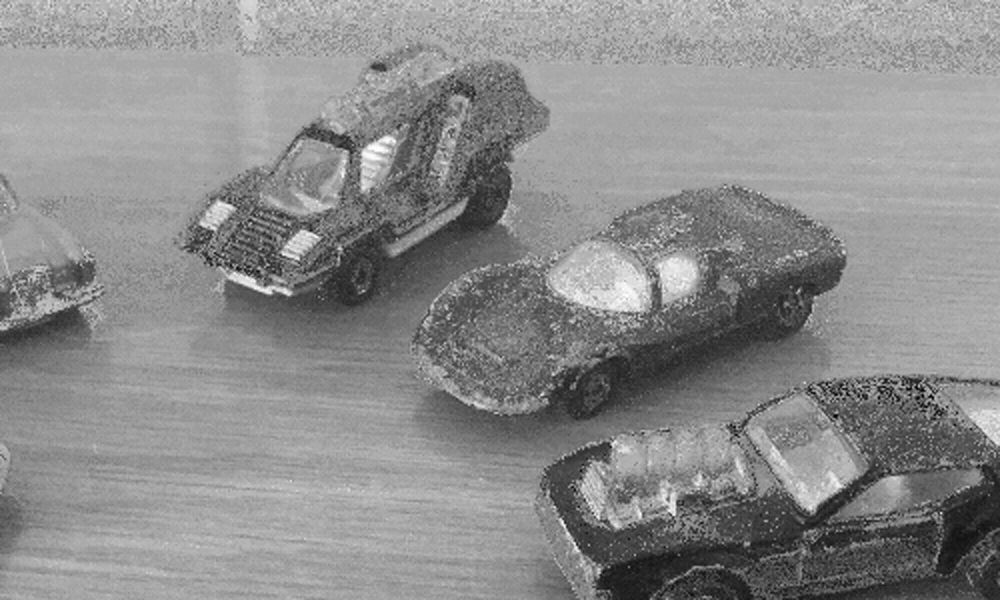
\includegraphics[width=\textwidth]{t5_zoom_R_knn.png}
        \caption{k-NN, no filter}
    \end{subfigure}
    \begin{subfigure}{0.32\textwidth}
        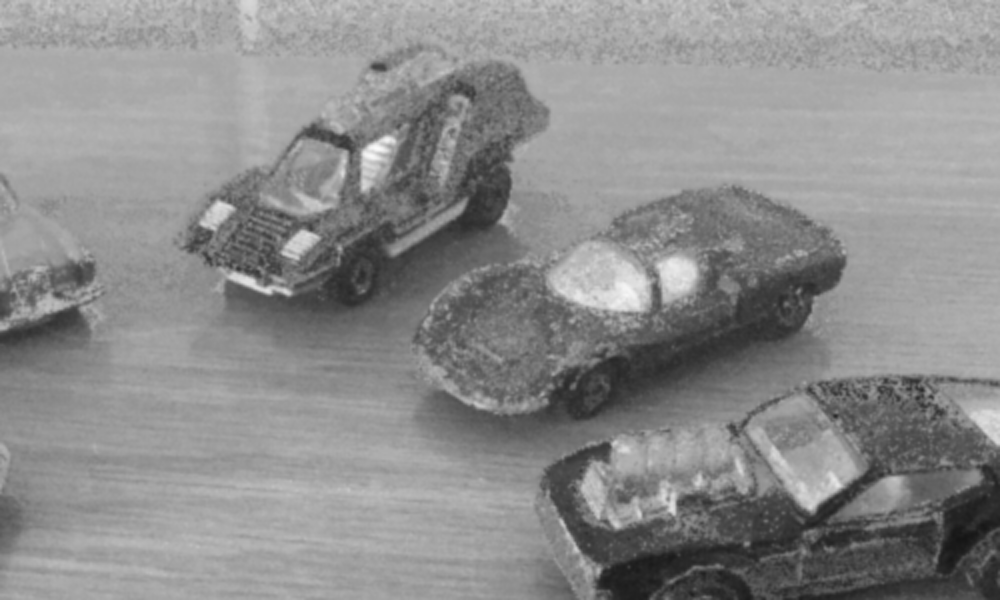
\includegraphics[width=\textwidth]{t5_zoom_R_knn_gaussian.png}
        \caption{Gaussian filter}
    \end{subfigure}
    \begin{subfigure}{0.32\textwidth}
        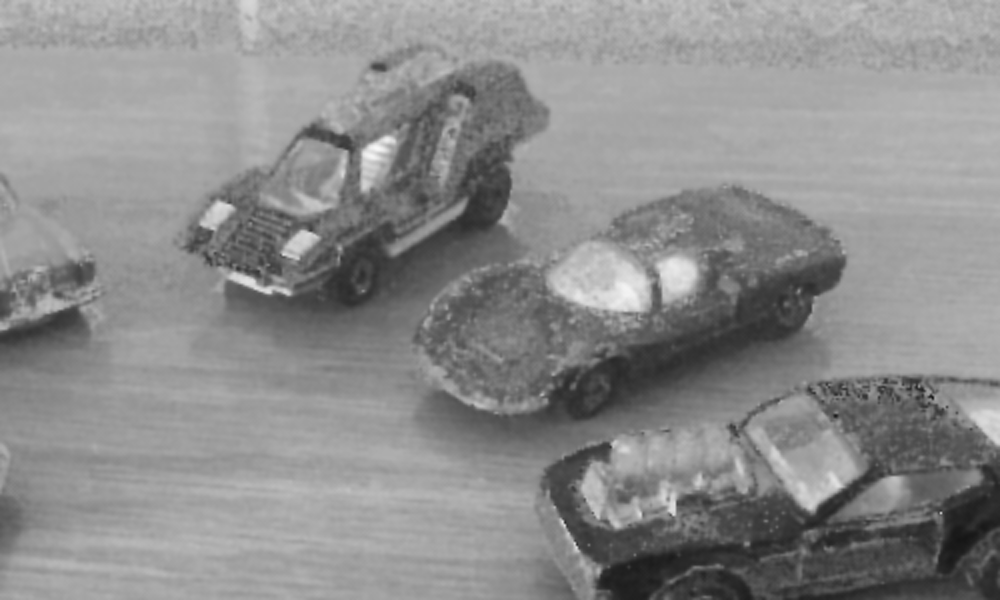
\includegraphics[width=\textwidth]{t5_zoom_R_knn_anisotropic.png}
        \caption{Anisotropic diffusion}
    \end{subfigure}
    \caption{Zoom on the estimated red channel (grey levels) of image 2 before and after the noise reduction.}
\end{figure}

\begin{figure}[H]
    \centering
    \begin{subfigure}{0.45\textwidth}
        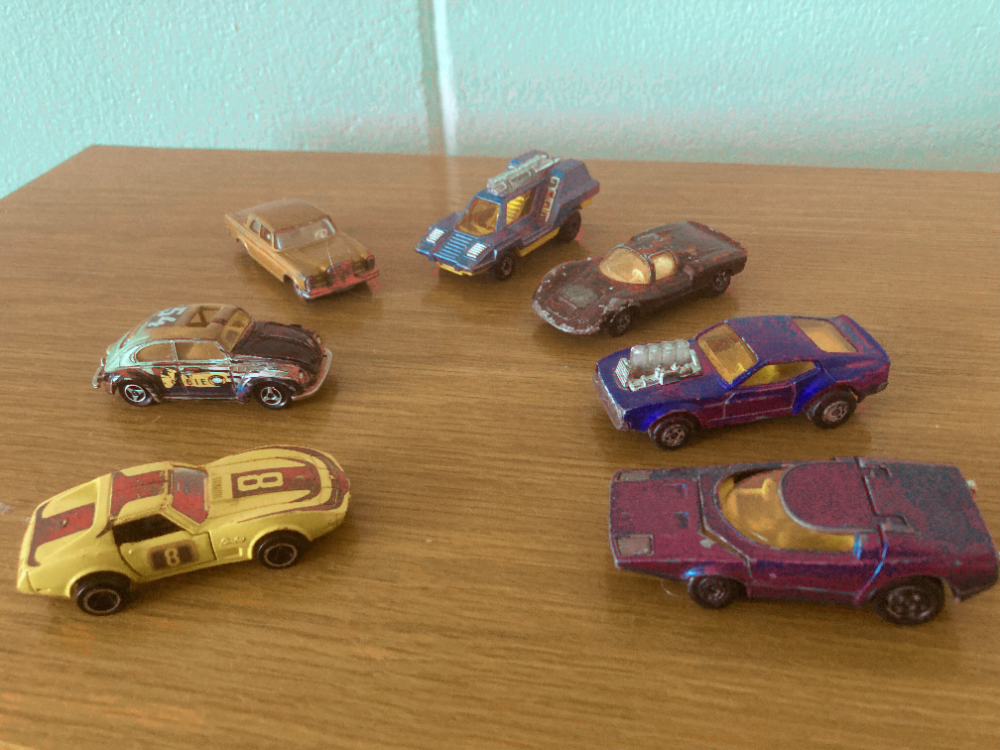
\includegraphics[width=\textwidth]{t5_knn_gaussian.png}
        \caption{k-NN and Gaussian filter}
    \end{subfigure}
    \begin{subfigure}{0.45\textwidth}
        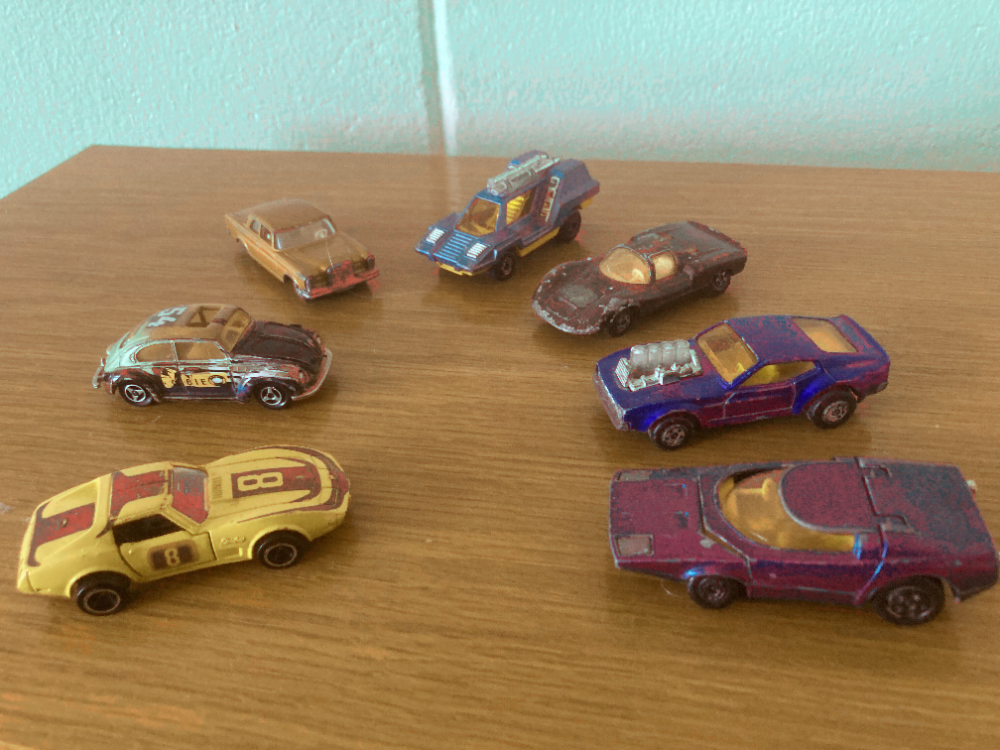
\includegraphics[width=\textwidth]{t5_knn_anisotropic.png}
        \caption{k-NN and anisotropic diffusion}
    \end{subfigure}
    \caption{Image 2 with the denoised red channel.}
\end{figure}

The methods make different errors: linear regression is good for the common colours and bad for the red cars, and k-NN is better for the red cars. We therefore averaged the red channels of linear regression and the denoised k-NN (anisotropic diffusion), and combined the average with the green and blue channels of image 2. RANSAC was left out, since it gave the same result as linear regression. The red stripes on the yellow car and the pink car keep a red tone, and the cyan tint of the wall is weaker than with k-NN alone. But the average also dilutes the red of k-NN with the values of the linear model, so the pink car is darker and more purple than with k-NN.

\begin{figure}[H]
    \centering
    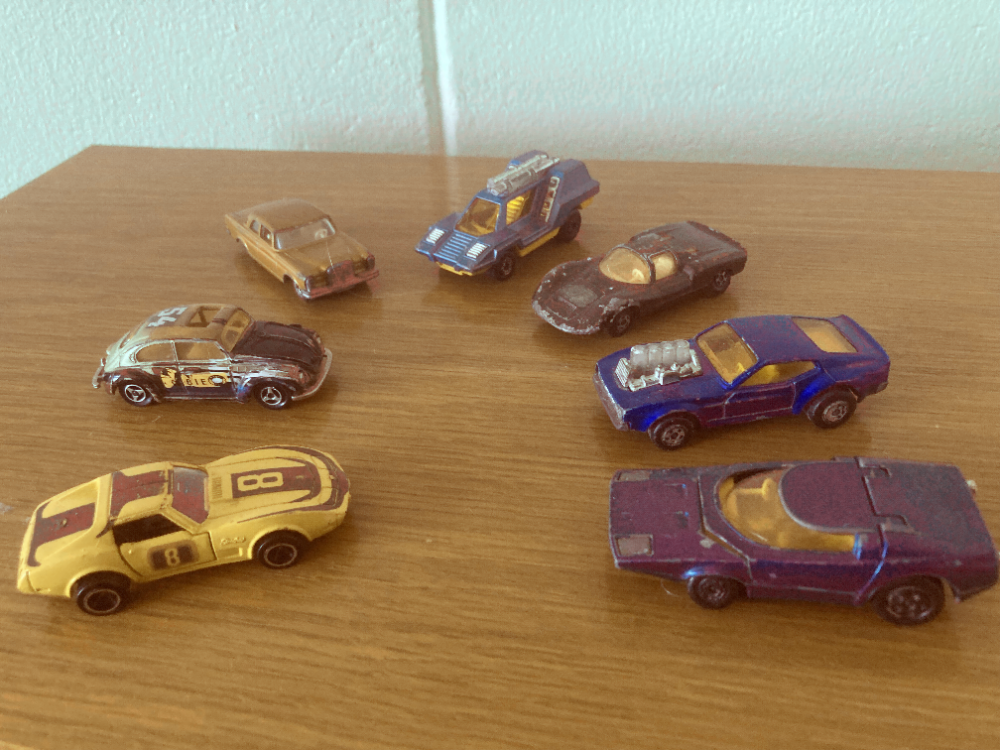
\includegraphics[width=0.7\textwidth]{t5_average.png}
    \caption{Image 2 with the average of the red channels of linear regression and the denoised k-NN.}
\end{figure}

Finally we compared the methods on the test set. With the chosen settings, each method learned from all the folds (5/6 of image 1) and was measured once on the test set, which had not been used for anything before.

\begin{center}
\begin{tabular}{lc}
\toprule
Method & RMSE \\
\midrule
Linear regression & 17.91 \\
RANSAC (threshold 80) & 17.94 \\
k-NN ($k = 100$) & 14.69 \\
k-NN, Gaussian filter ($\sigma = 0.7$) & \textbf{13.24} \\
k-NN, anisotropic diffusion (2 iterations, $\kappa = 100$) & 13.33 \\
Average (linear regression, denoised k-NN) & 14.47 \\
\bottomrule
\end{tabular}
\end{center}

k-NN is clearly better than linear regression and RANSAC, and the filtering improves its RMSE. RANSAC is the same as linear regression, as the cross-validation showed. The average is better than linear regression but worse than the denoised k-NN alone. 

All three methods use only the green and blue value of one pixel, and this does not determine the red value. A better result needs information that is not in the colour of one pixel, for example the surroundings of the pixel, or a match between the two images that lets the red channel be copied from image 1.


\section{Task 6: Finding the way to the rocket}

The idea is to turn the picture into a directed graph and search it. The nodes are the places where arrows and footprints meet, each arrow is an edge from the node at its tail to the node at its head, and the craters tell which nodes are not allowed.

\textbf{Craters.} The craters are dark ellipse-shaped outlines. We threshold the dark ink, keep the large blobs and fit ellipses to their outlines with RANSAC. The ellipses are constrained to the shape of a crater (size, aspect ratio and tilt), and we only accept an ellipse if it covers enough of the outline and has the orange colour of the crater inside. The ellipses are enlarged a little to cover the whole outline. This gave 10 craters.

\begin{figure}[H]
    \centering
    \begin{subfigure}{0.32\textwidth}
        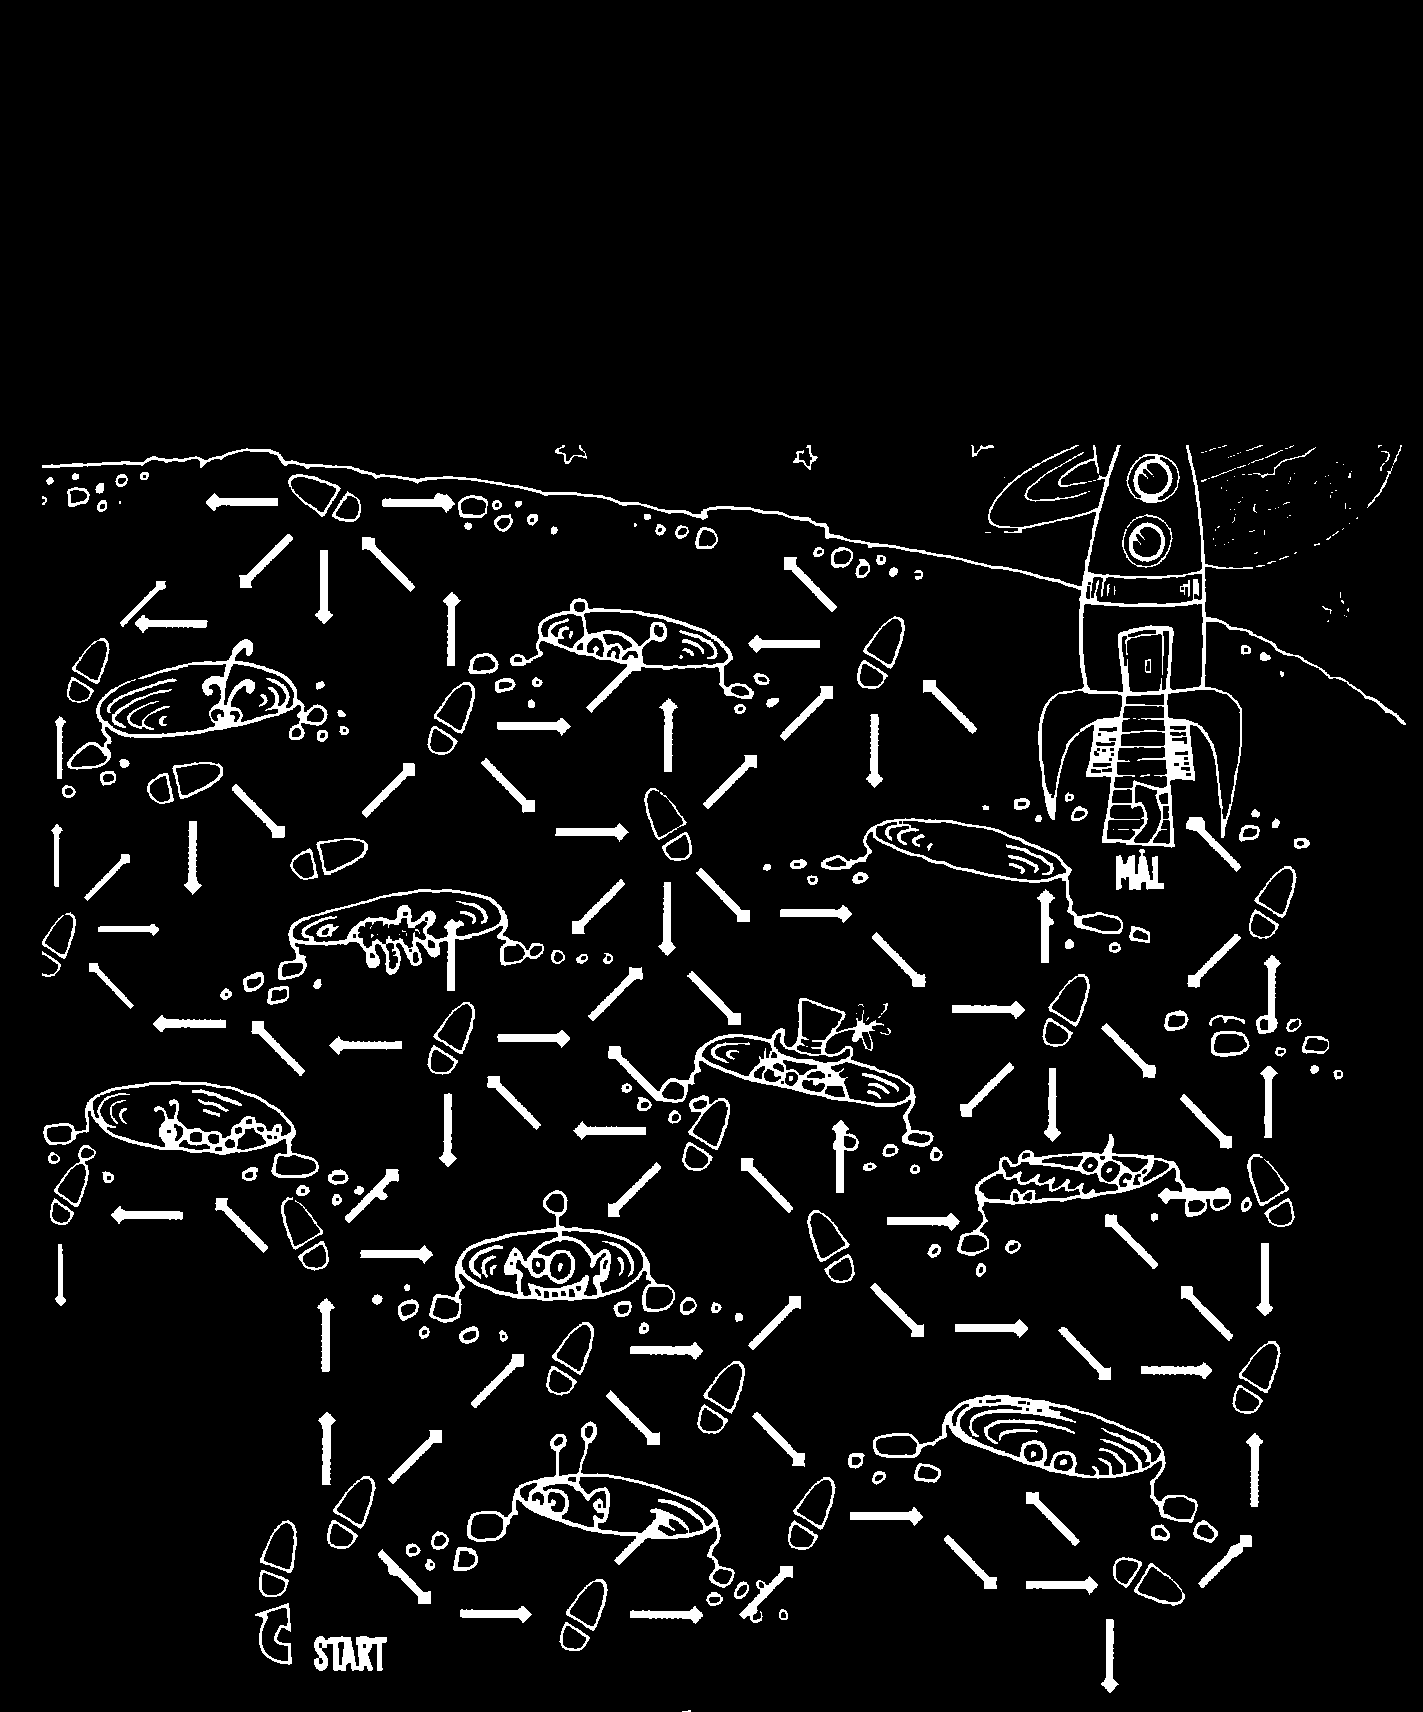
\includegraphics[width=\textwidth]{t6_01_dark_ink.png}
        \caption{Dark ink}
    \end{subfigure}
    \begin{subfigure}{0.32\textwidth}
        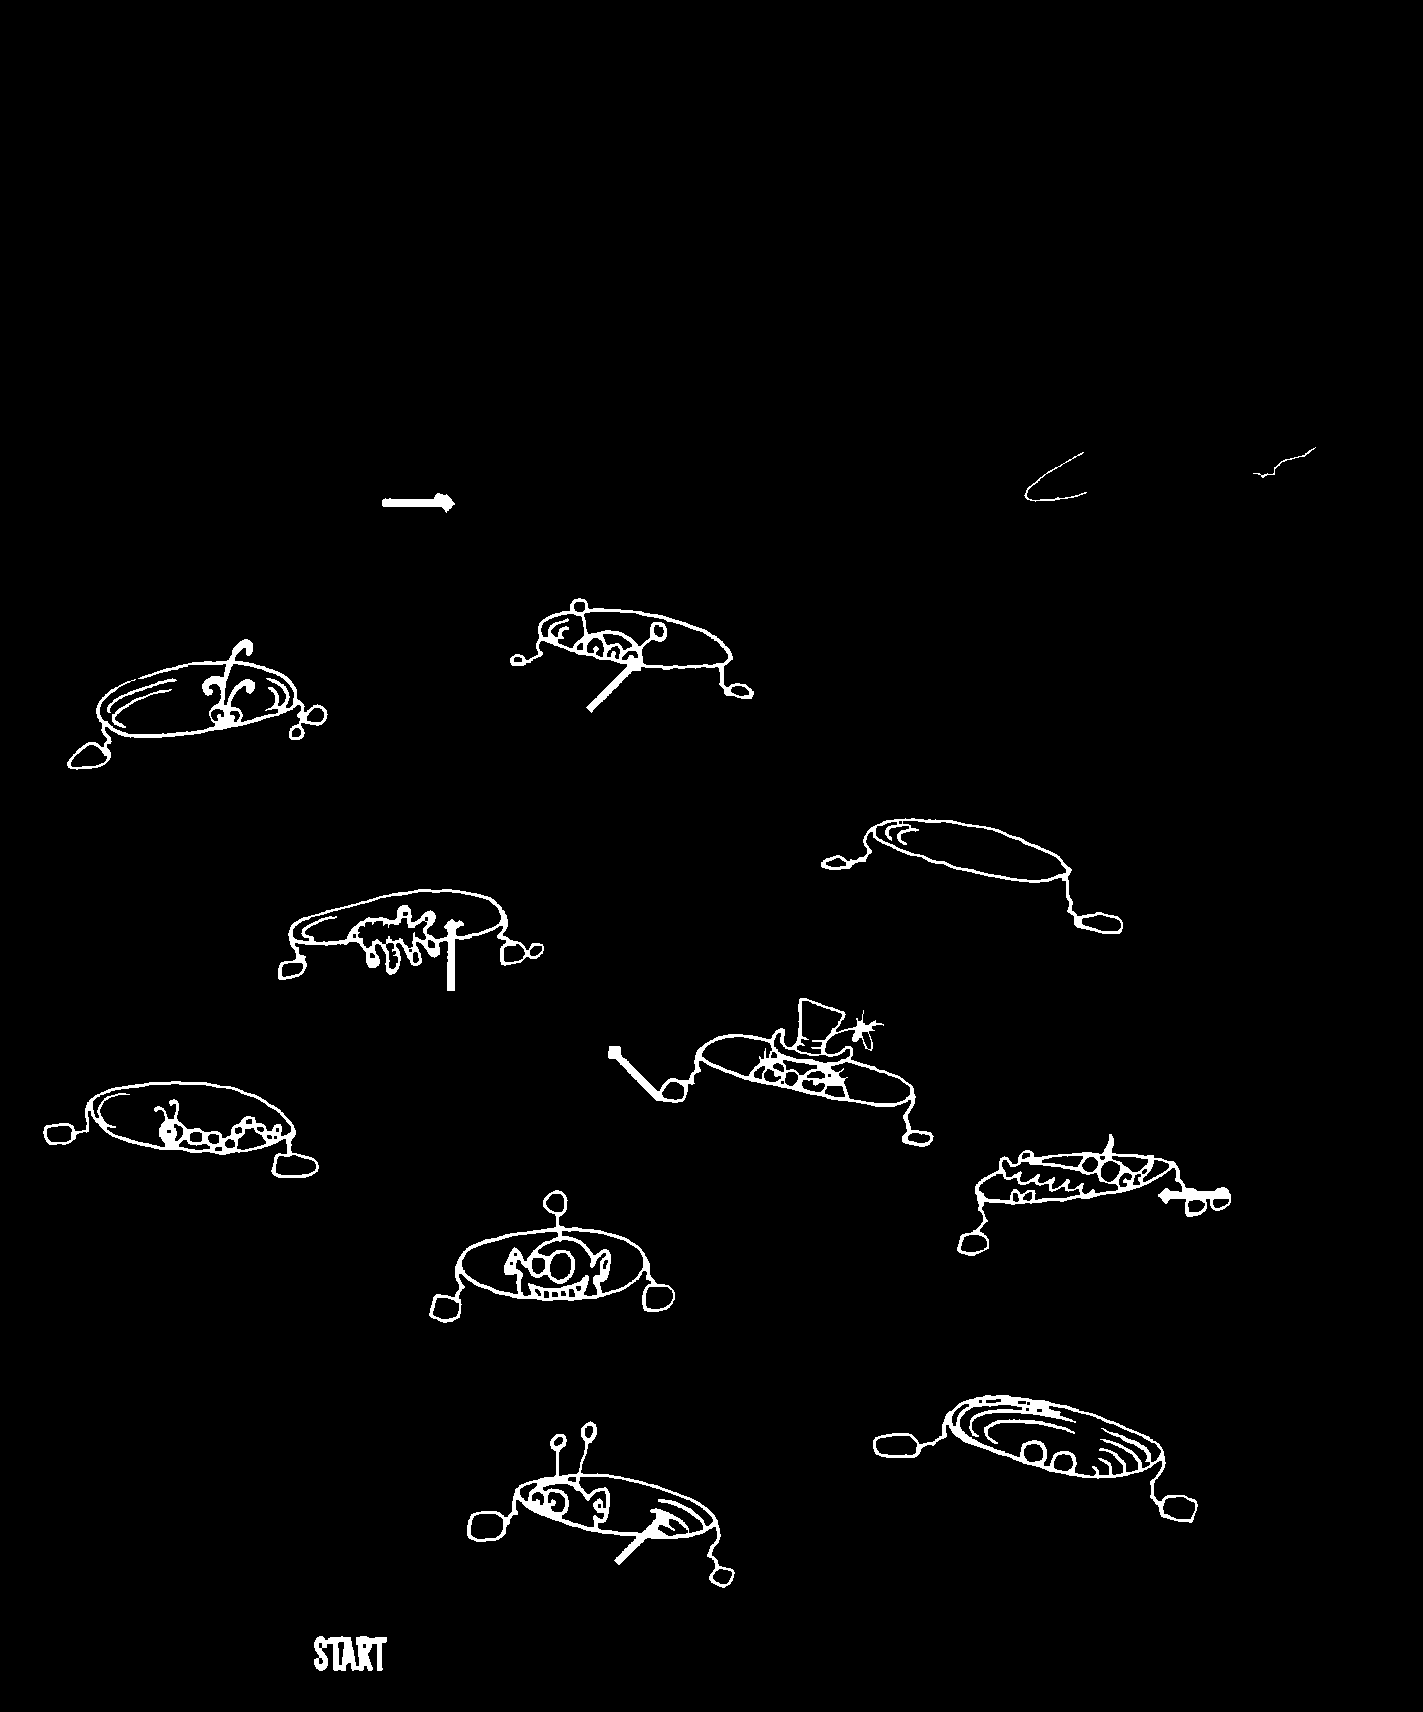
\includegraphics[width=\textwidth]{t6_02_big_ink_blobs.png}
        \caption{Large blobs}
    \end{subfigure}
    \begin{subfigure}{0.32\textwidth}
        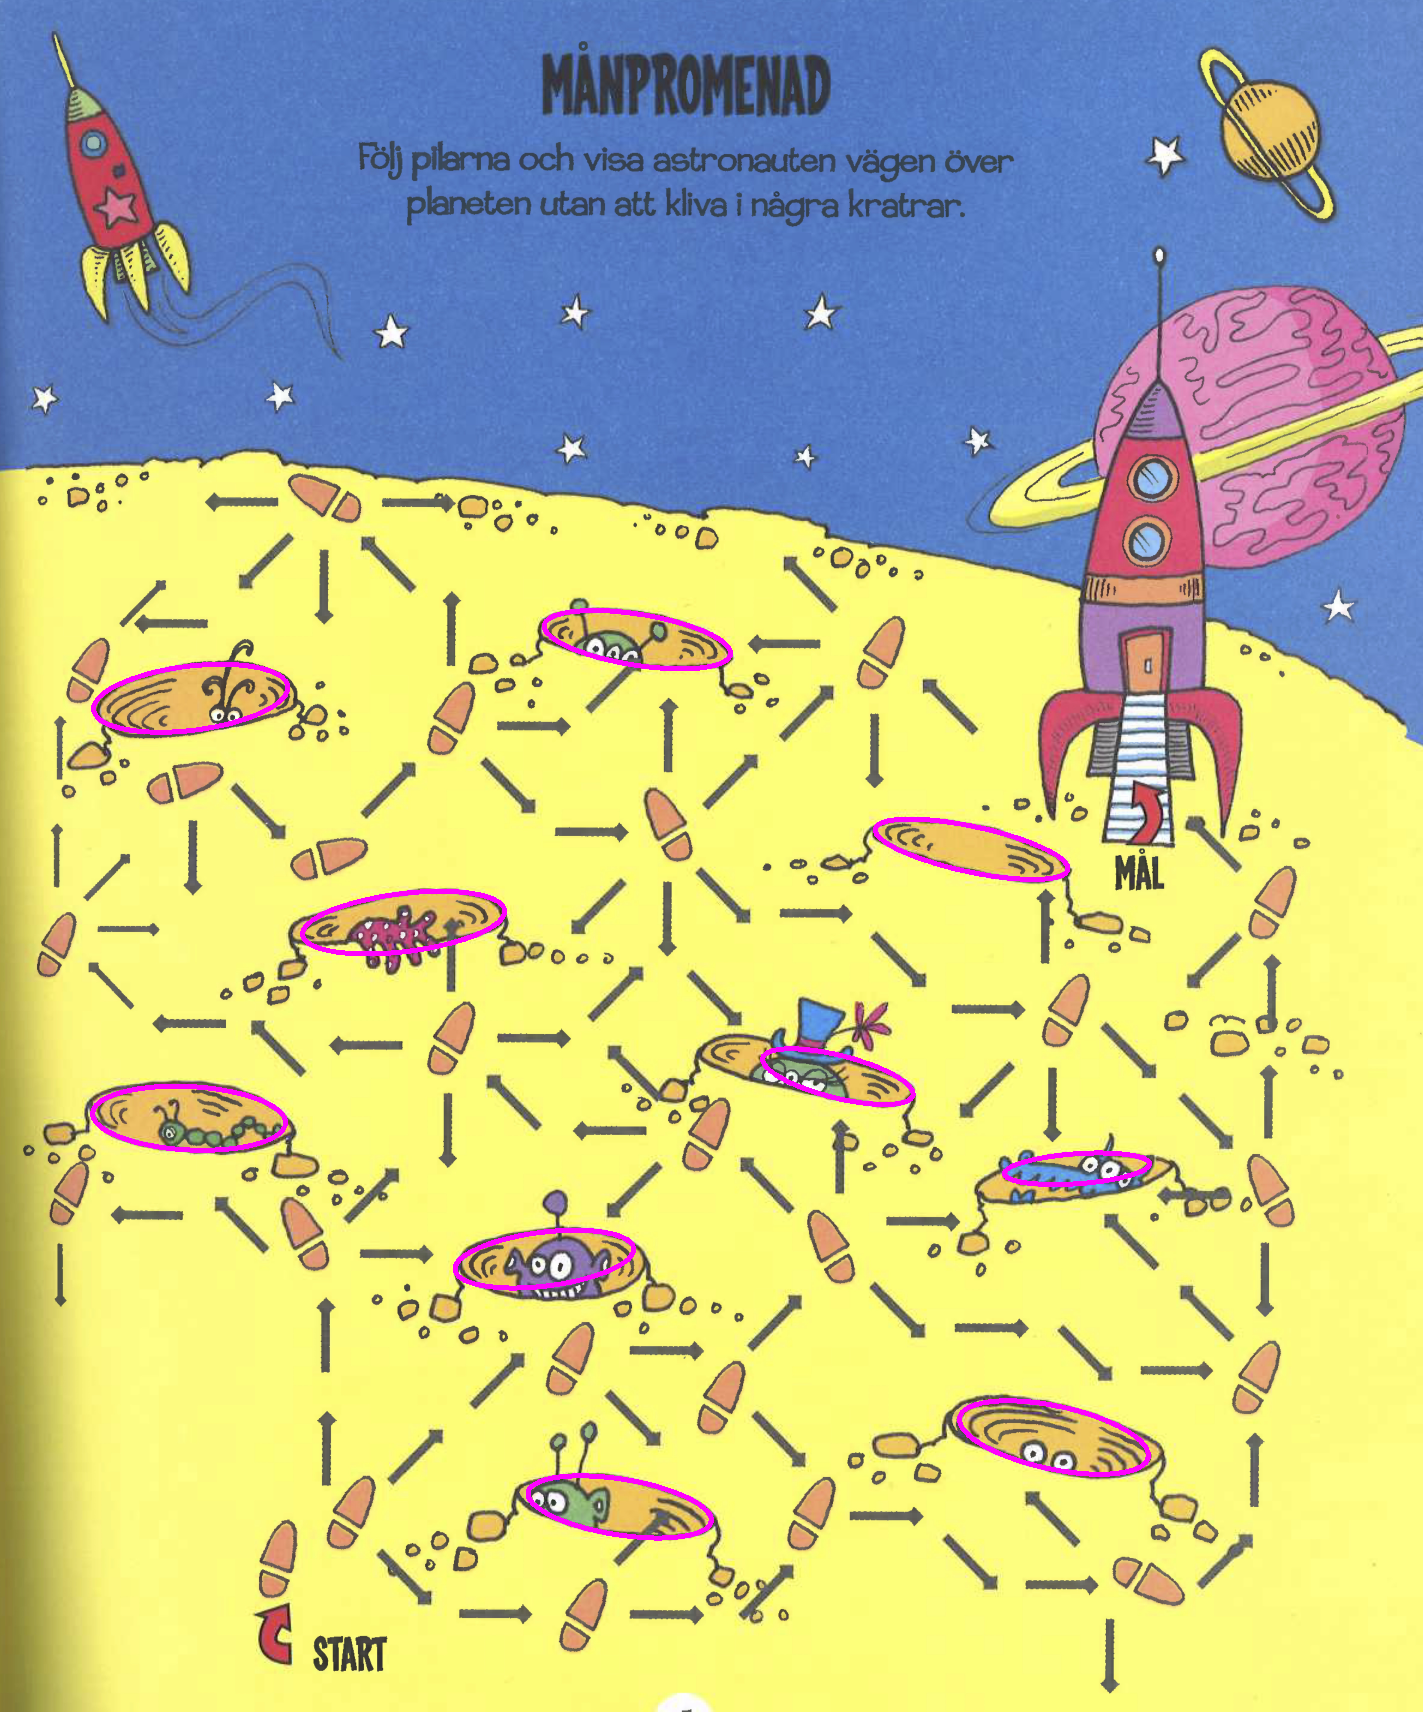
\includegraphics[width=\textwidth]{t6_03_fitted_ellipses.png}
        \caption{Fitted ellipses}
    \end{subfigure}
    \caption{Steps of the crater detection.}
\end{figure}

\textbf{Arrows.} The arrows are dark gray. We threshold the gray image, clean the mask with a closing and an opening, and take each connected component as one arrow. The direction of an arrow is found with PCA: the first principal axis gives the line of the arrow, and the head is the end of the axis where there are more pixels, since the head is wider than the tail. The yellow ring that surrounds an arrow is used to reject components that are not arrows (for example the letter L of MÅL). We found 87 arrows. Arrows that lie inside craters are not needed, since the craters are forbidden.

\begin{figure}[H]
    \centering
    \begin{subfigure}{0.32\textwidth}
        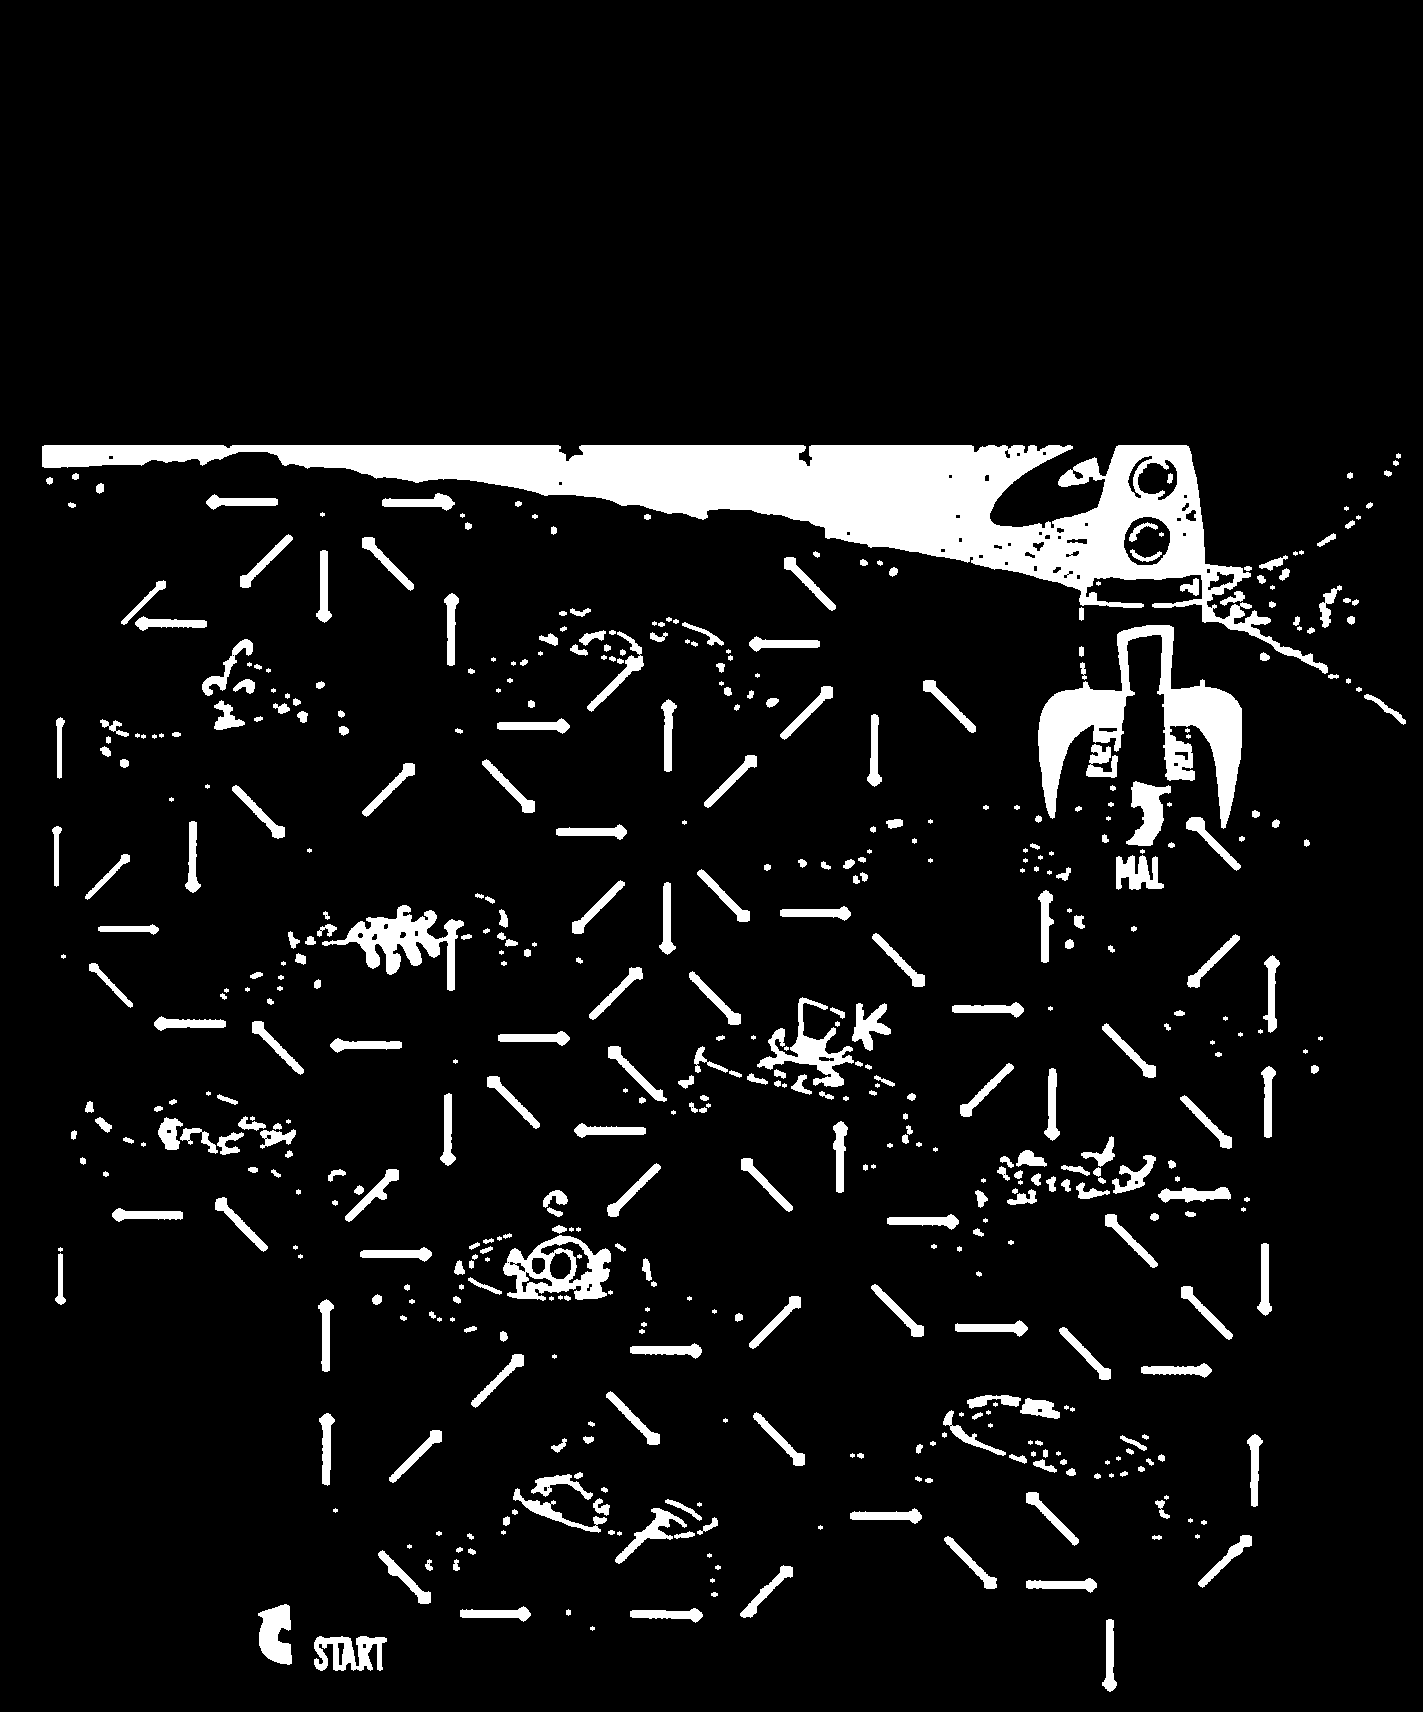
\includegraphics[width=\textwidth]{t6_06_dark_ink_mask.png}
        \caption{Gray mask}
    \end{subfigure}
    \begin{subfigure}{0.32\textwidth}
        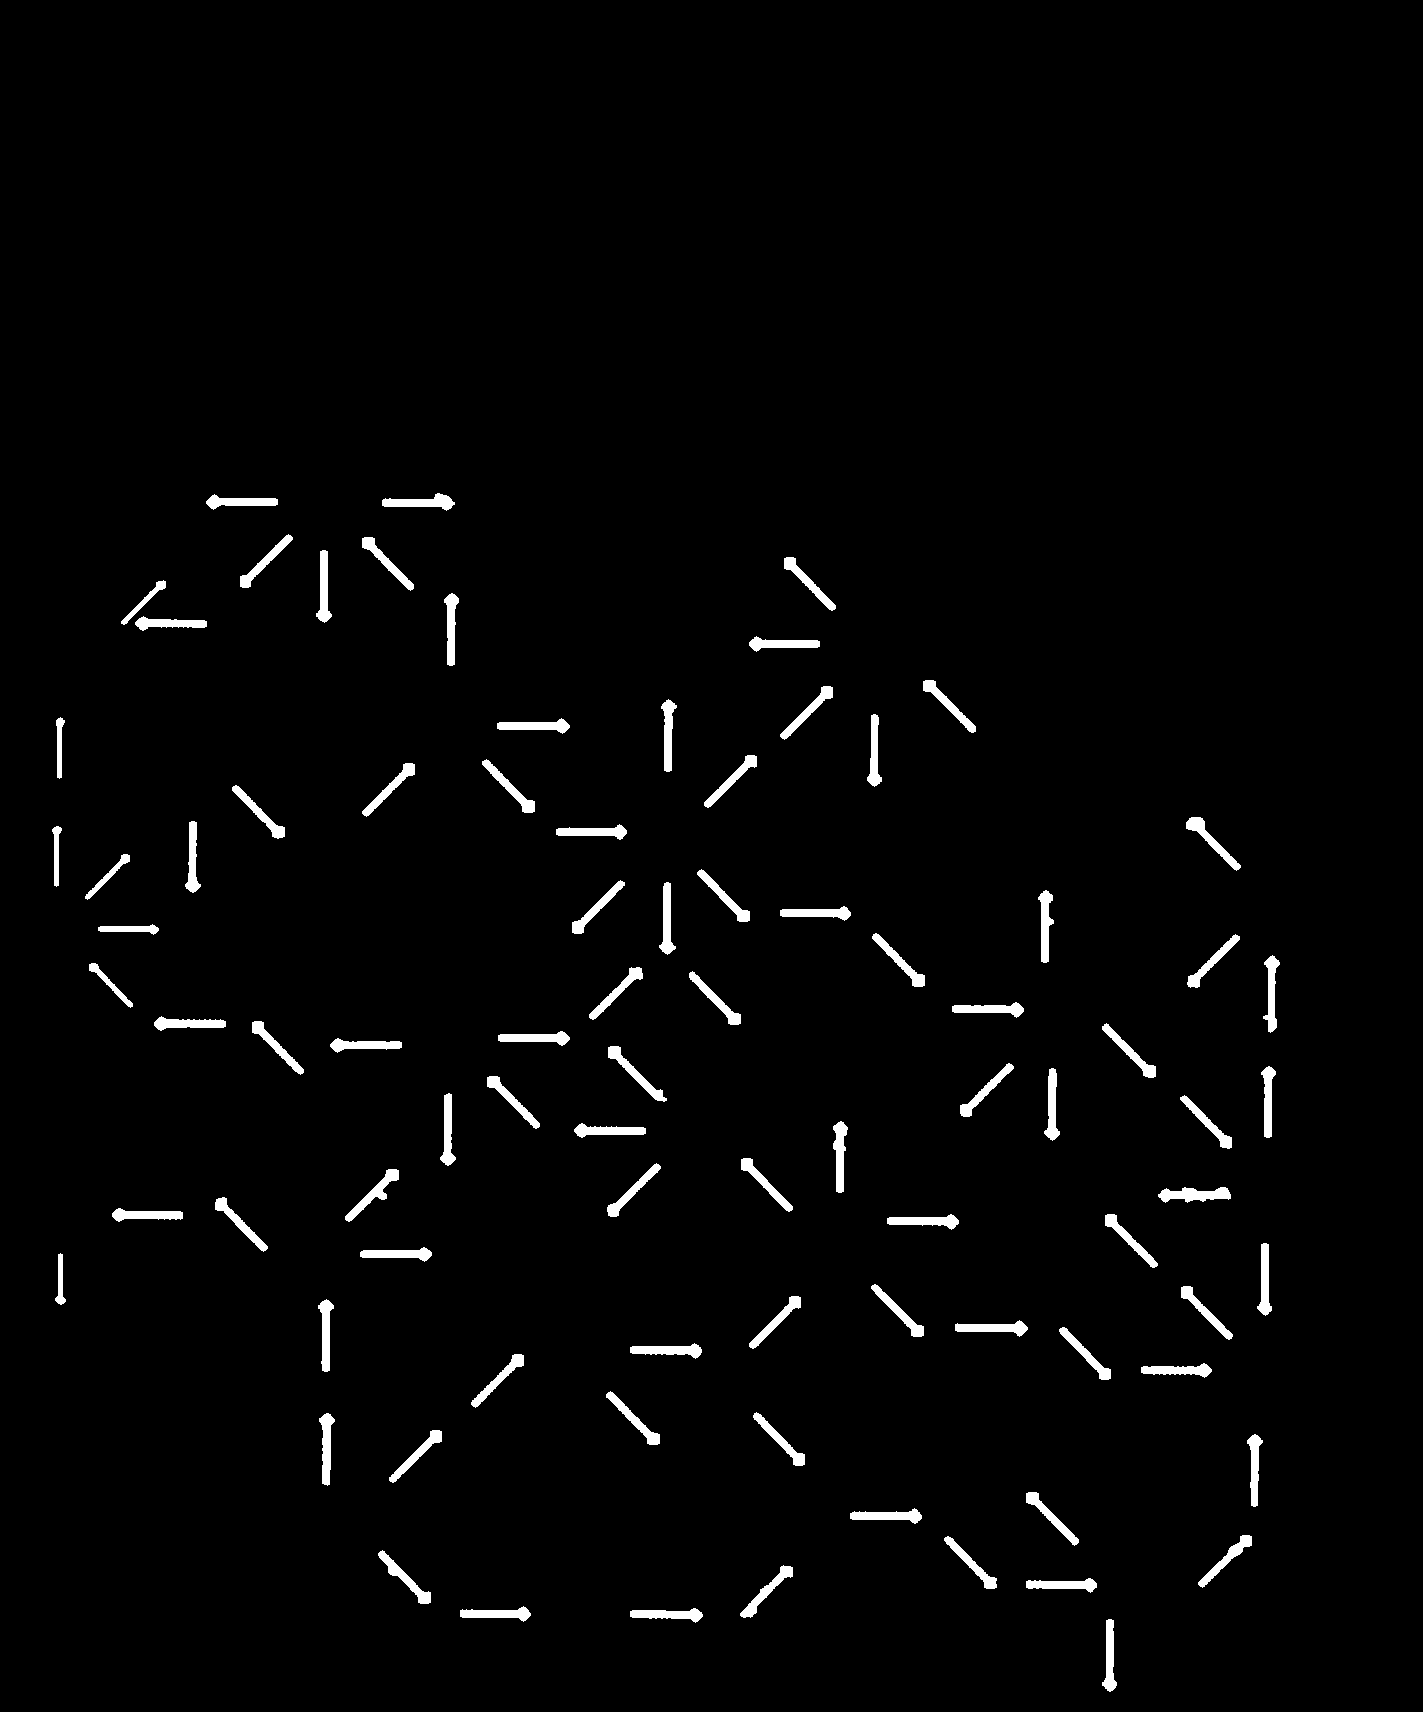
\includegraphics[width=\textwidth]{t6_08_arrow_mask.png}
        \caption{Arrow blobs}
    \end{subfigure}
    \begin{subfigure}{0.32\textwidth}
        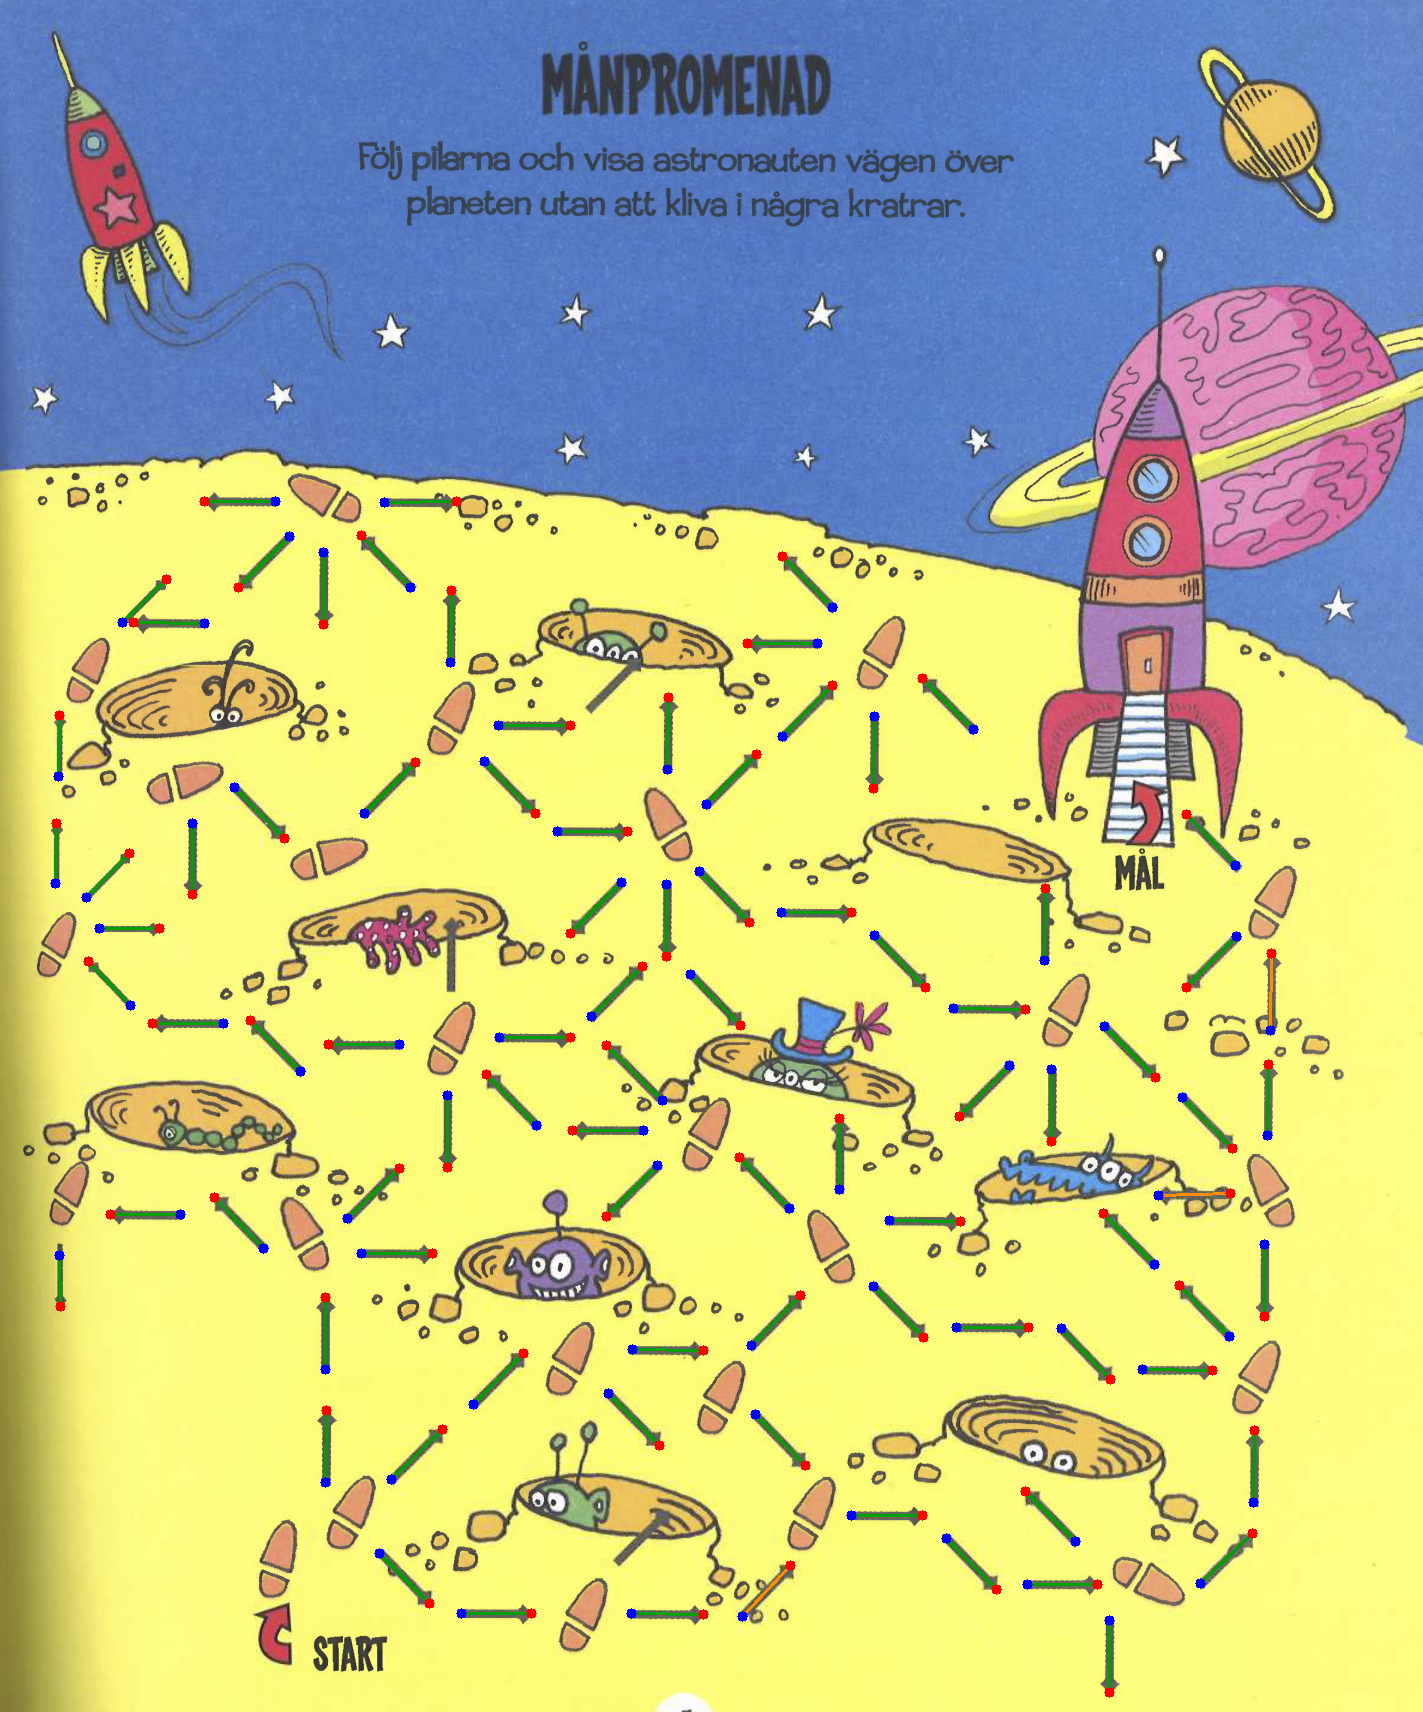
\includegraphics[width=\textwidth]{t6_09_arrow_directions.png}
        \caption{Directions, tail to head}
    \end{subfigure}
    \caption{Steps of the arrow detection.}
\end{figure}

\textbf{Footprints.} The footprints are orange. We threshold the orange pixels, close and fill the footprint shapes, and keep the components that have a footprint size and shape. We found 24 footprints.

\begin{figure}[H]
    \centering
    \begin{subfigure}{0.32\textwidth}
        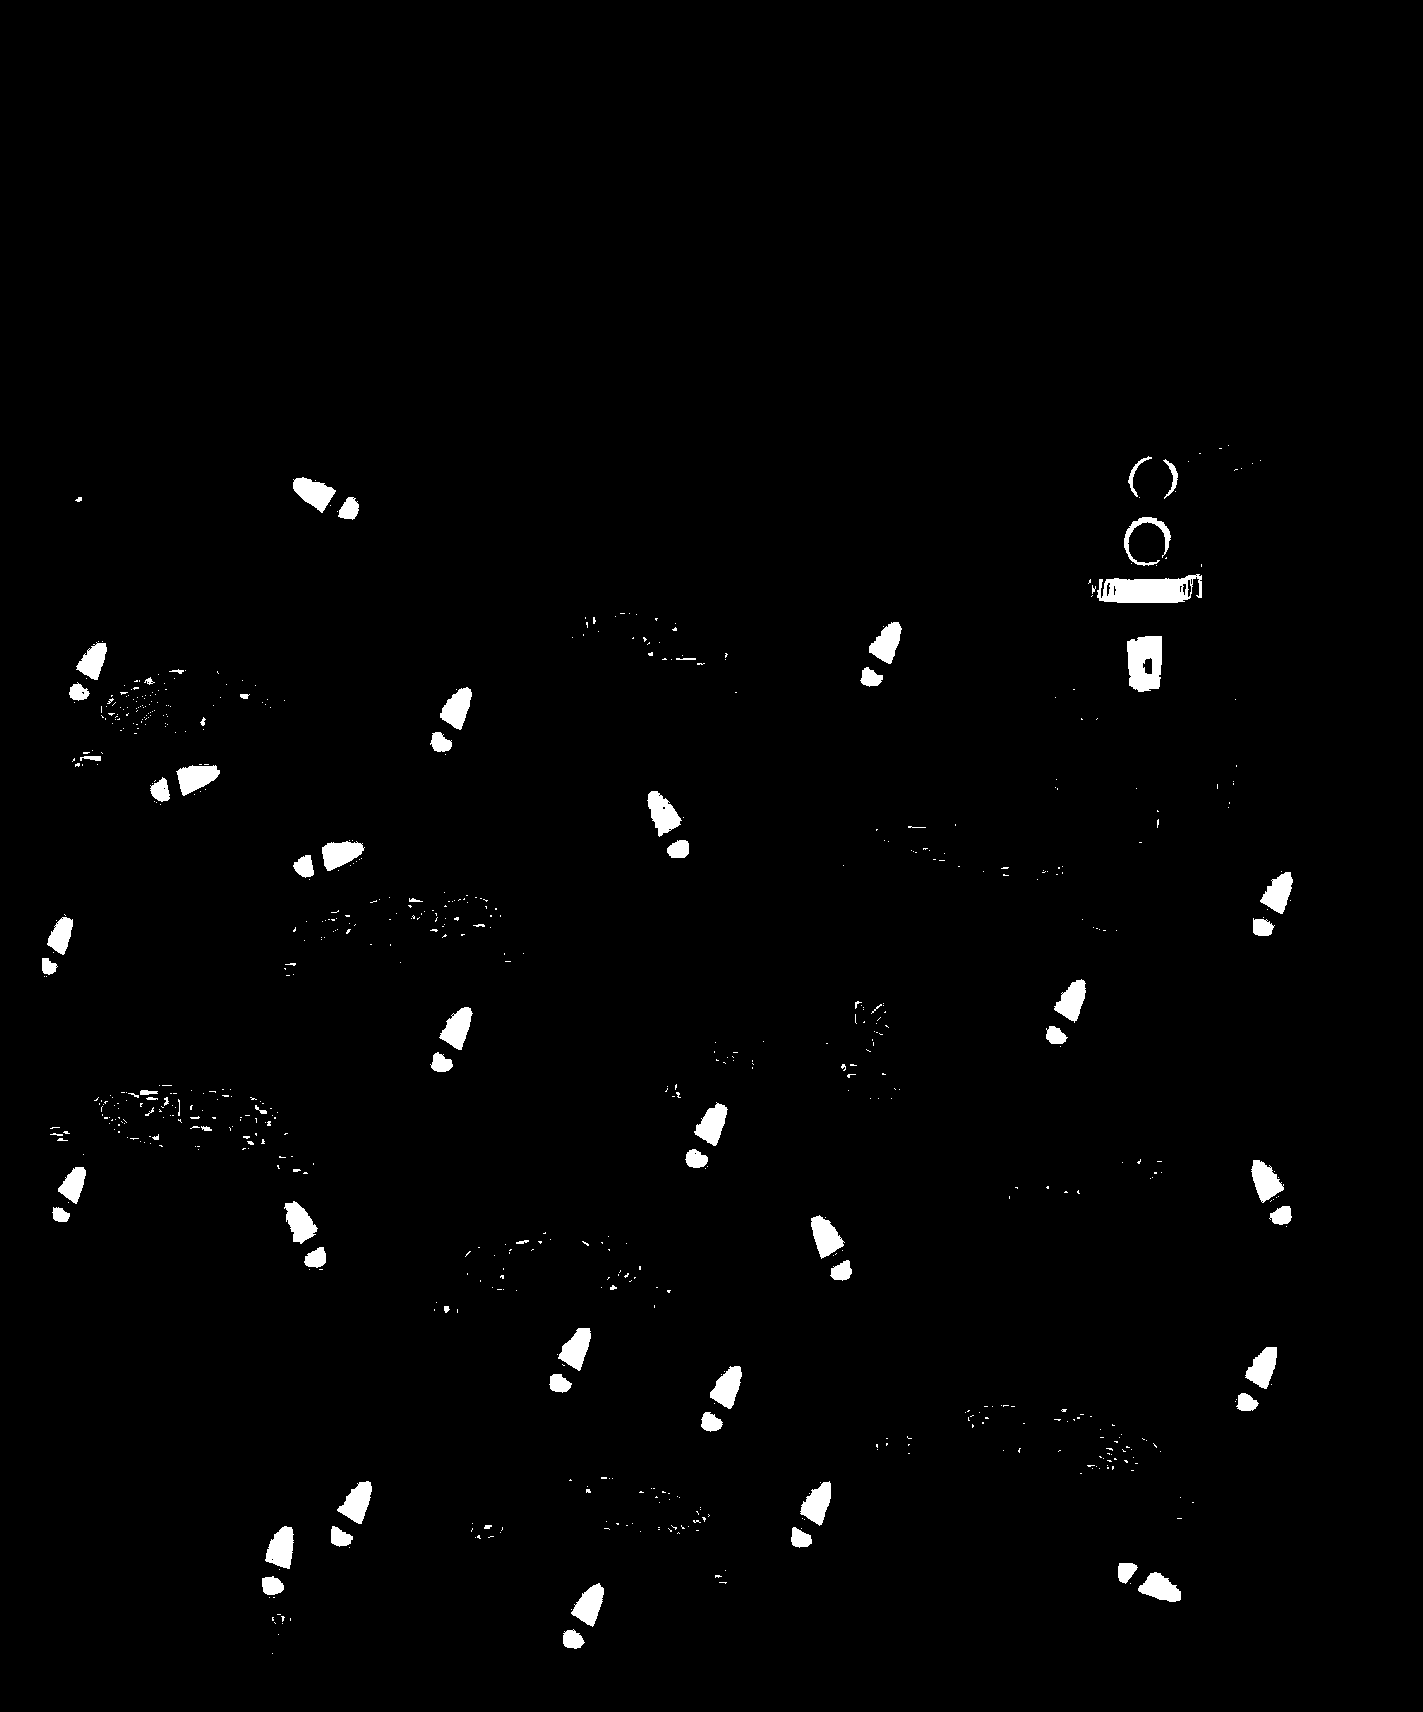
\includegraphics[width=\textwidth]{t6_10_orange_pixels.png}
        \caption{Orange pixels}
    \end{subfigure}
    \begin{subfigure}{0.32\textwidth}
        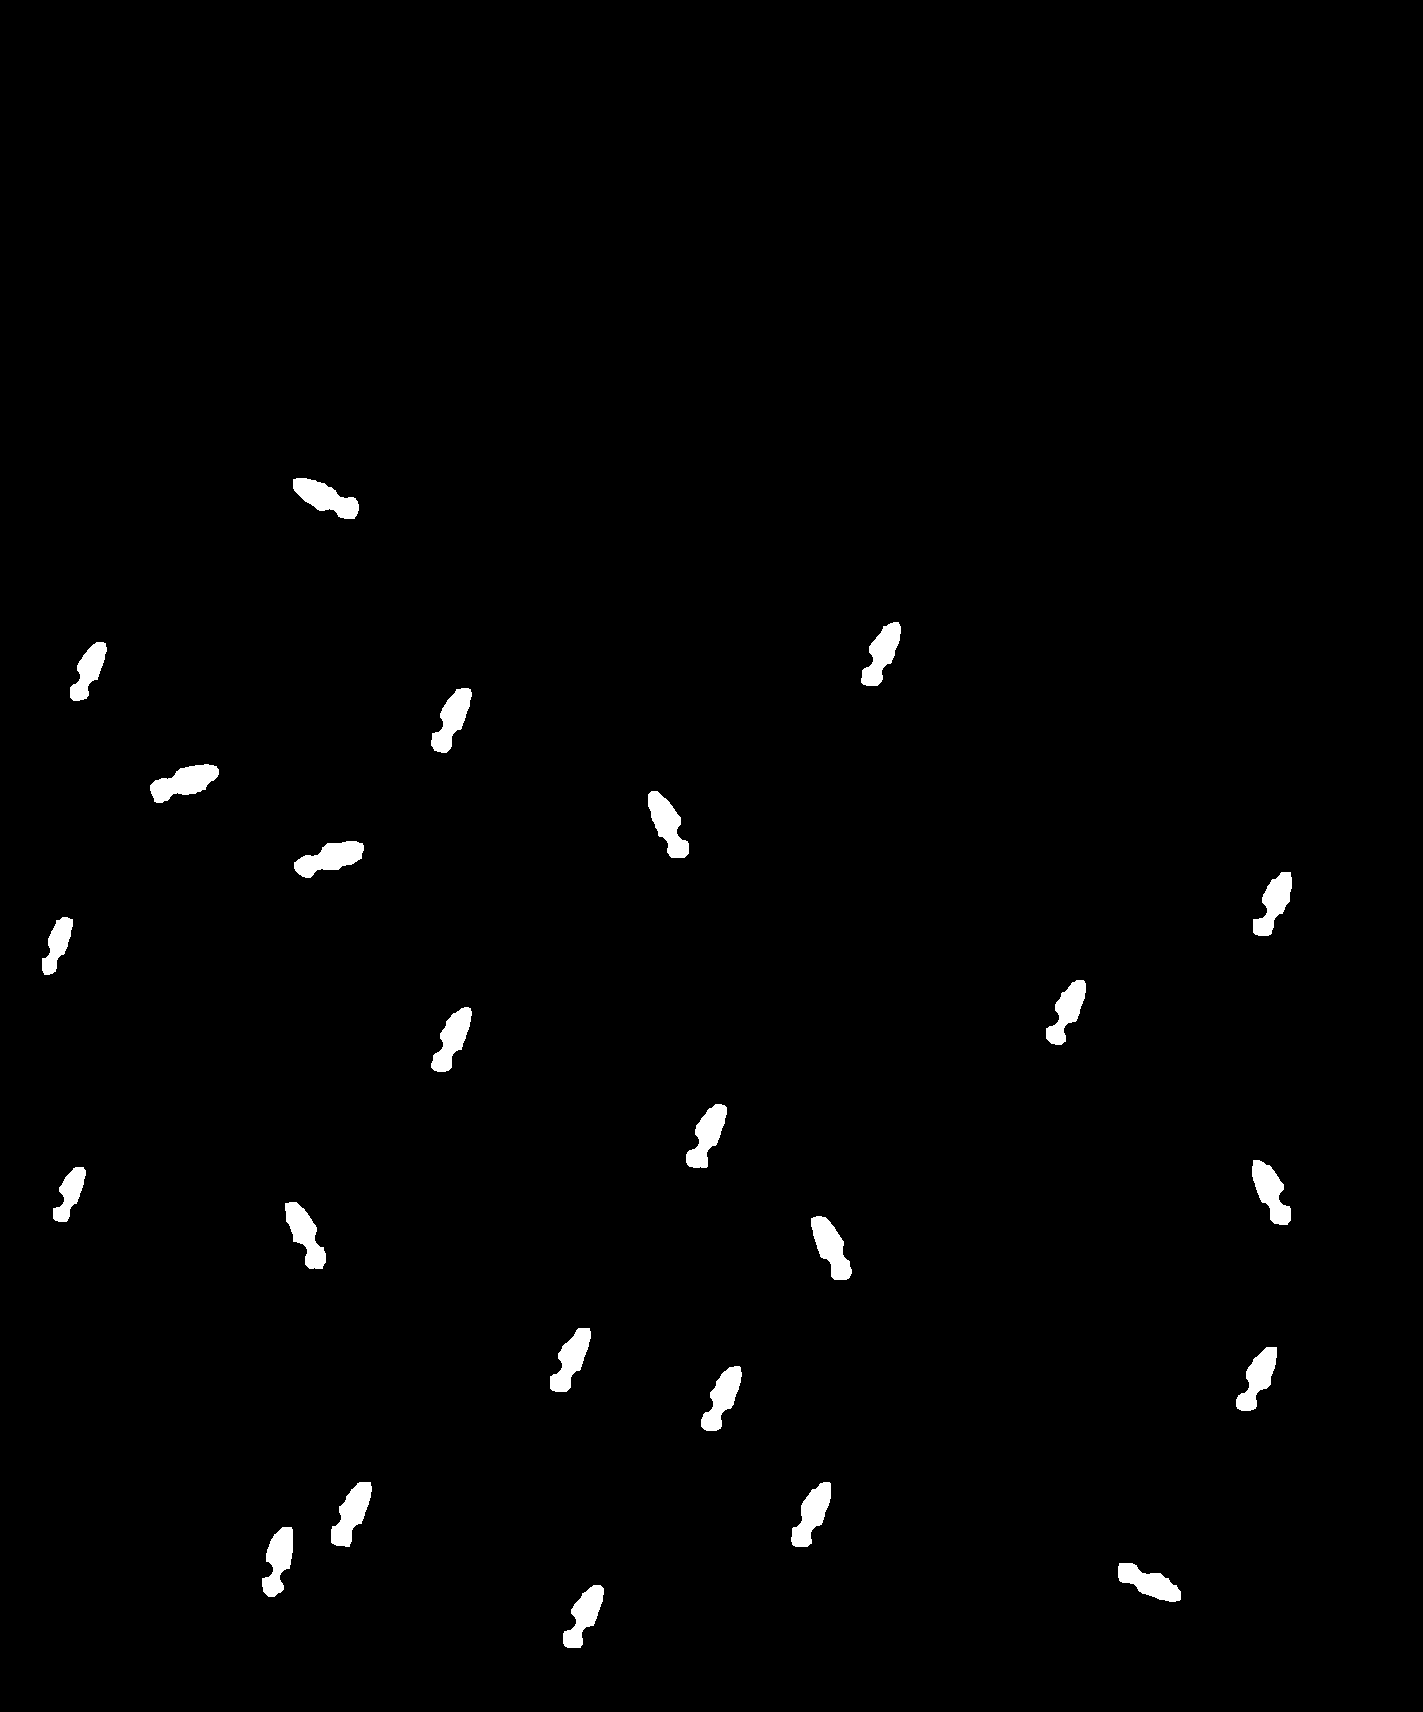
\includegraphics[width=\textwidth]{t6_11_footprints.png}
        \caption{Footprints}
    \end{subfigure}
    \begin{subfigure}{0.32\textwidth}
        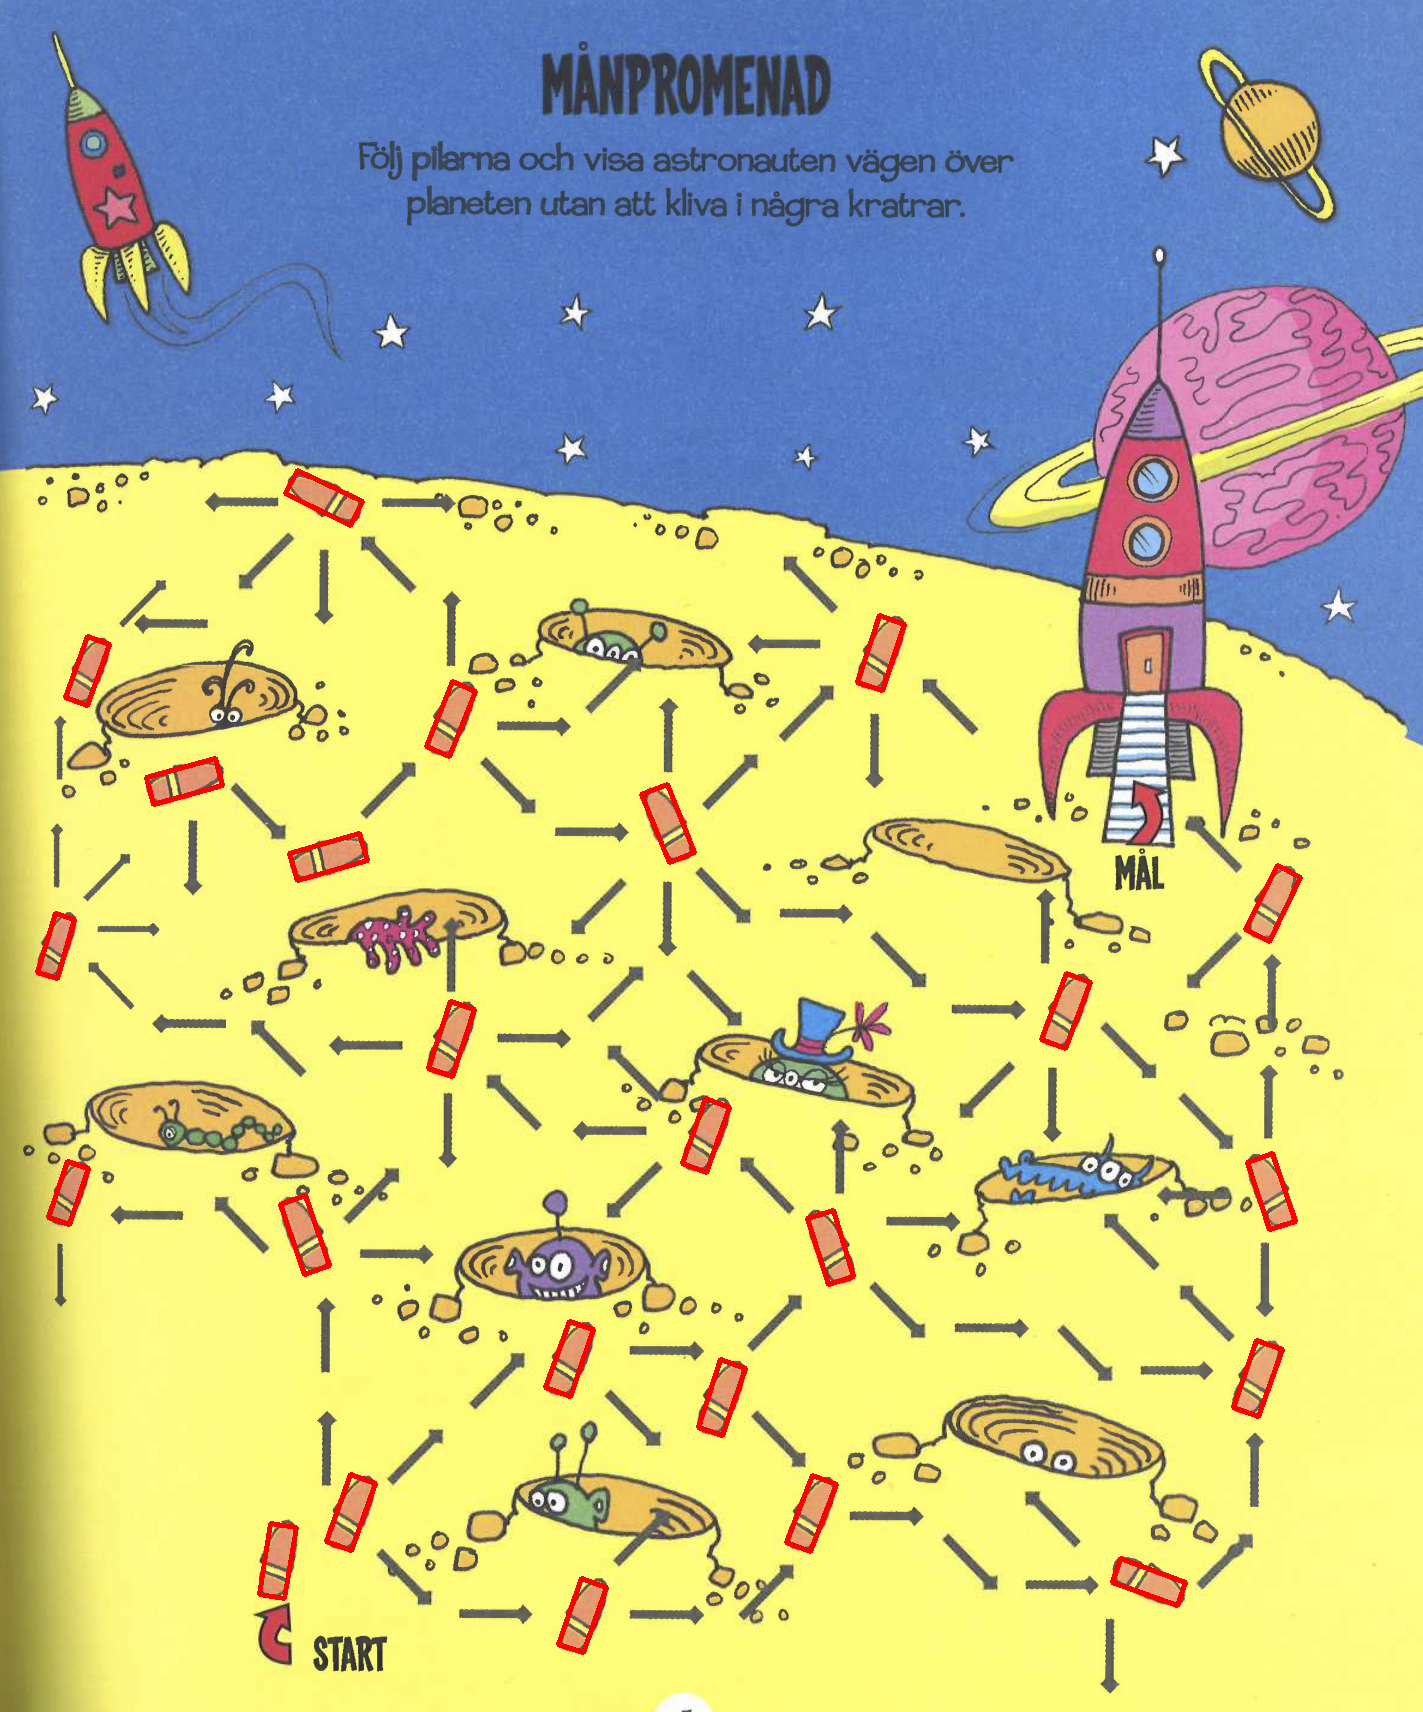
\includegraphics[width=\textwidth]{t6_12_footprints_on_image.png}
        \caption{Footprints on the image}
    \end{subfigure}
    \caption{Steps of the footprint detection.}
\end{figure}

\textbf{Start and goal.} START and MÅL are marked with a red icon each. We threshold the red pixels and clean the mask with an opening and a closing. The other red things (the rocket, the pink alien) are removed because the icons are small and taller than wide. The lower of the two icons found is START and the other is MÅL.

\begin{figure}[H]
    \centering
    \begin{subfigure}{0.35\textwidth}
        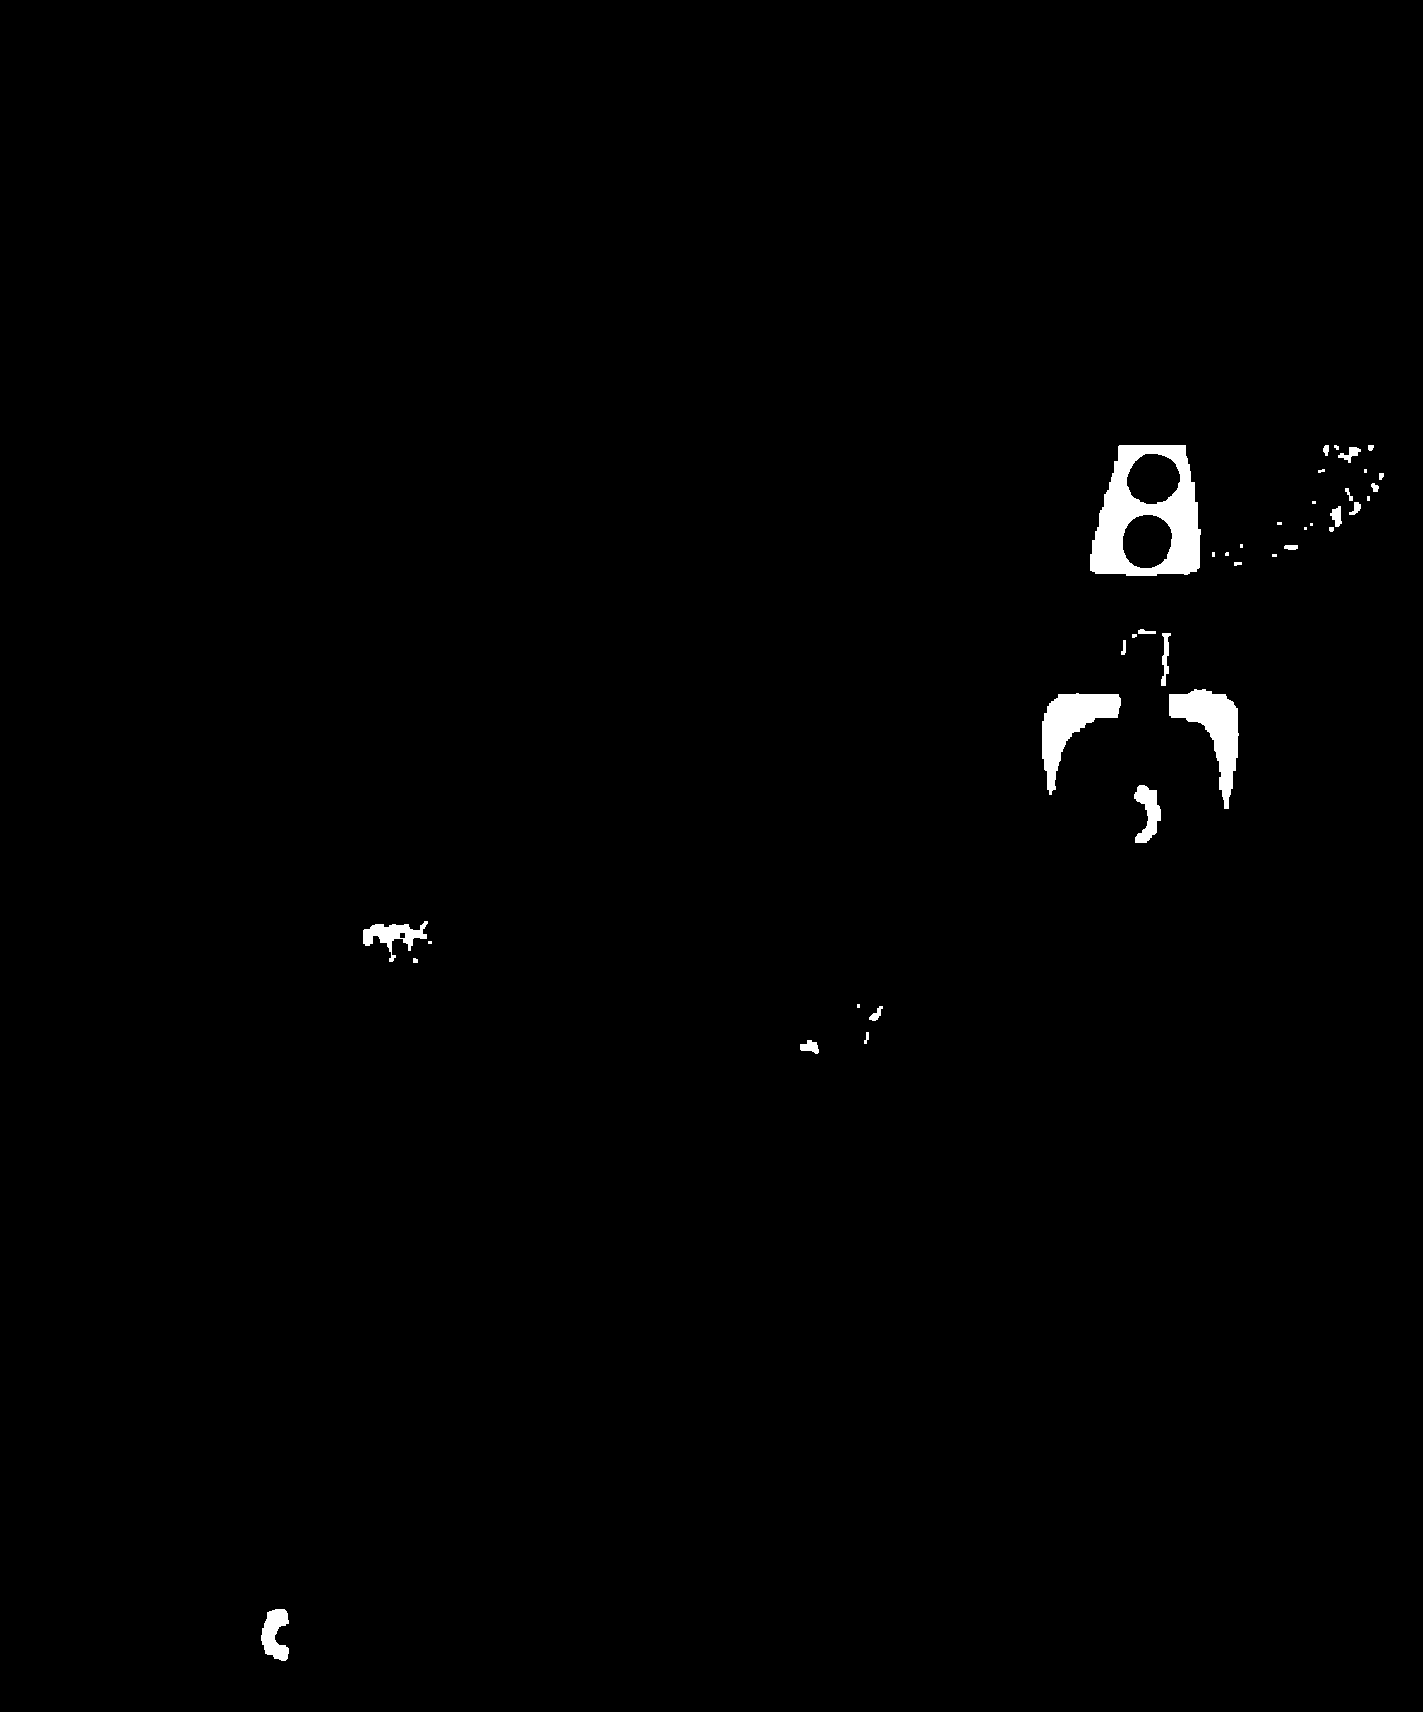
\includegraphics[width=\textwidth]{t6_13_red_pixels.png}
        \caption{Red pixels}
    \end{subfigure}
    \begin{subfigure}{0.35\textwidth}
        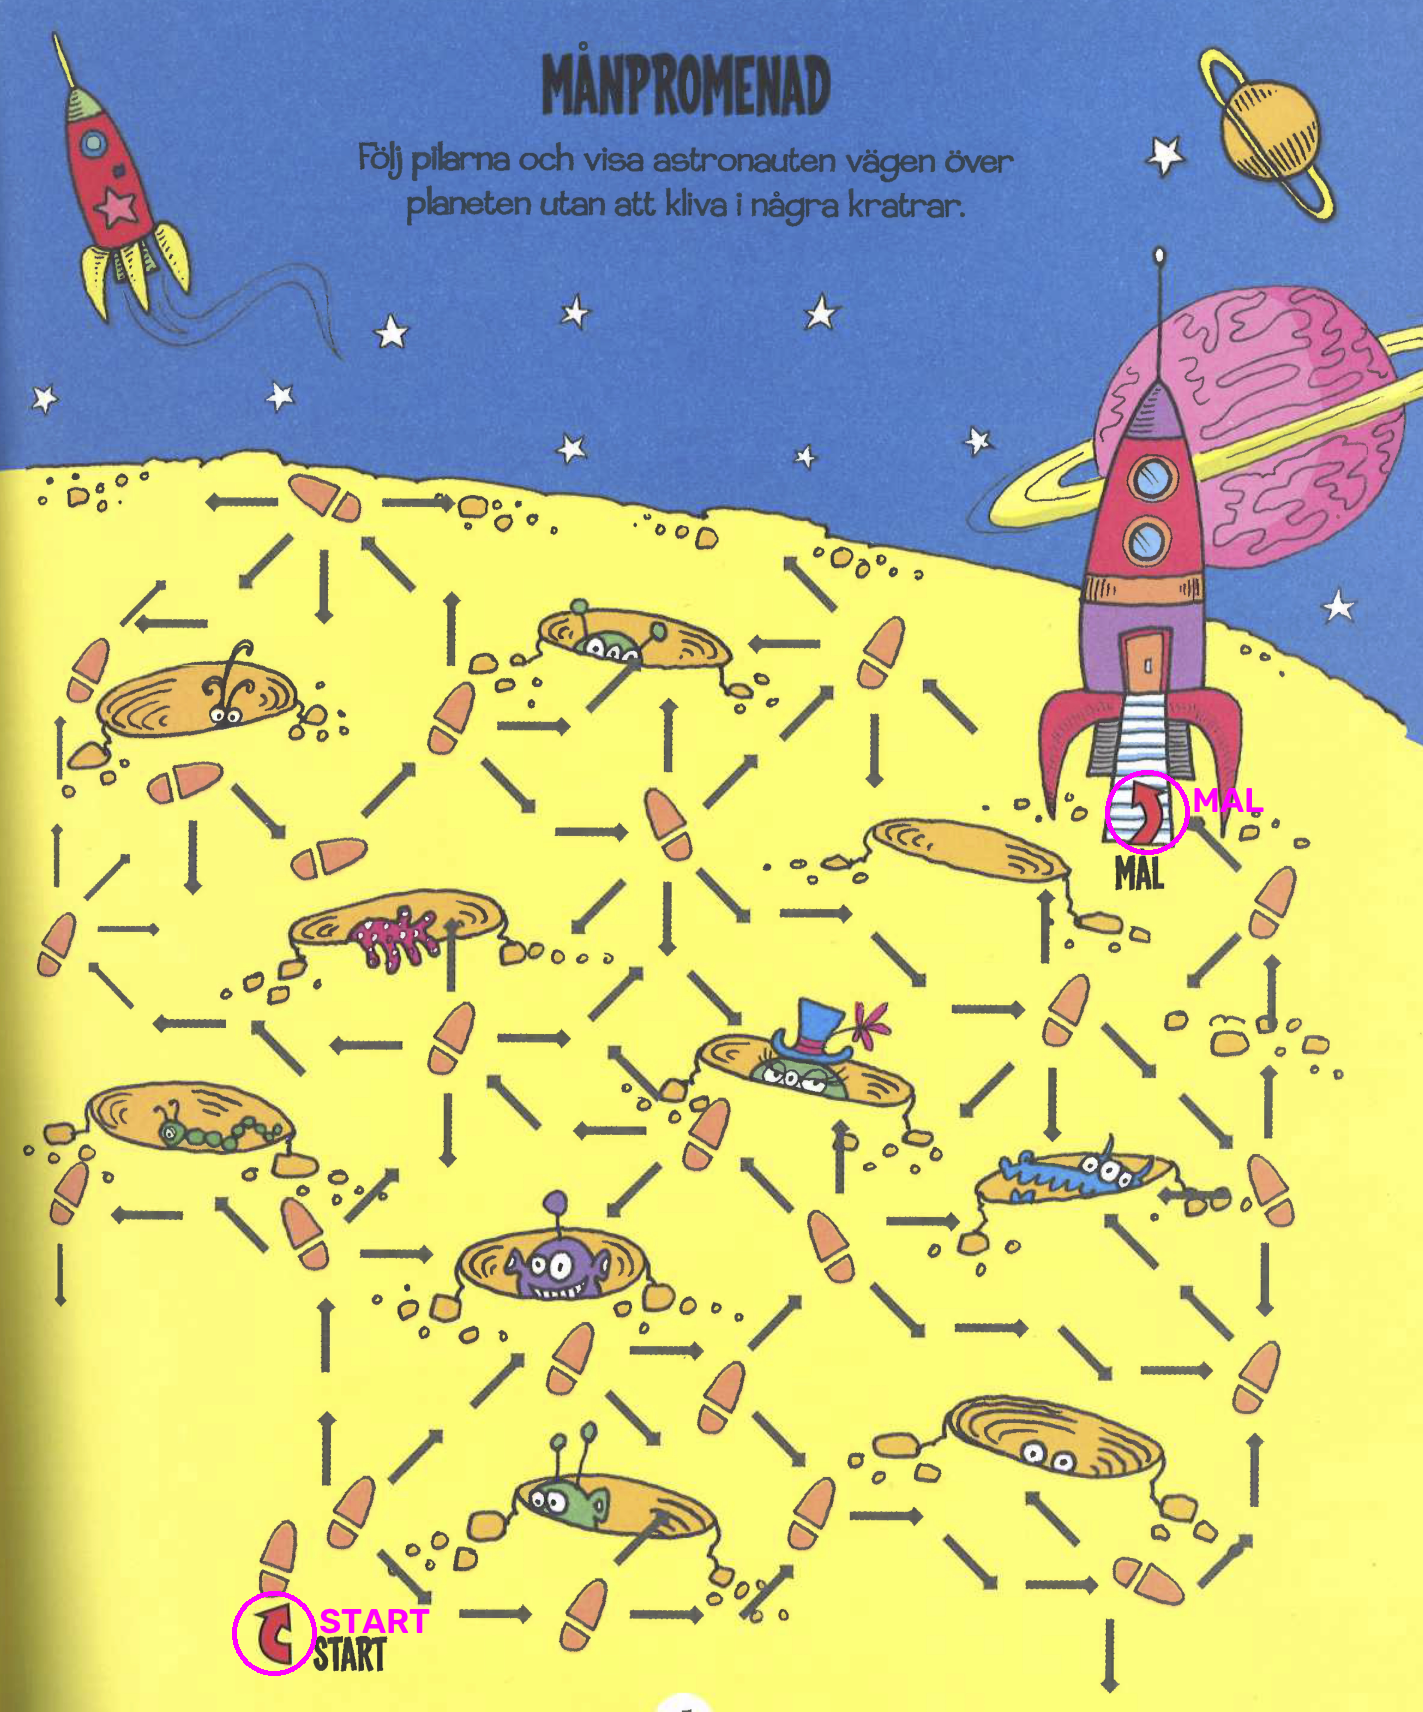
\includegraphics[width=\textwidth]{t6_14_start_and_goal.png}
        \caption{START and MÅL}
    \end{subfigure}
    \caption{Finding START and MÅL.}
\end{figure}

\textbf{Nodes.} To find them, every footprint is dilated by 30 pixels, and a disc of radius 28 pixels is drawn around the head and around the tail of every arrow. Areas that touch each other belong together, so the connected components of all the grown areas are the candidates for nodes. We got 76 candidates.

A candidate is a node only if it follows these rules:
\begin{itemize}
    \item It has at least one arrow head and at least one arrow tail. A candidate with only heads, only tails, only heads and a footprint, or only tails and a footprint is a dead end or a start of nothing, so it is not a node.
    \item It does not touch a crater, since we must avoid the craters.
    \item A candidate that contains a footprint is always a node, even if its grown area touches the margin of a crater.
    \item The candidates next to the START and MÅL icons are always nodes, even if they have only heads or only tails.
\end{itemize}
Of the 76 candidates, 52 are nodes. 11 were rejected for touching a crater, 12 for having only heads and 1 for having only tails.

\begin{figure}[H]
    \centering
    \begin{subfigure}{0.35\textwidth}
        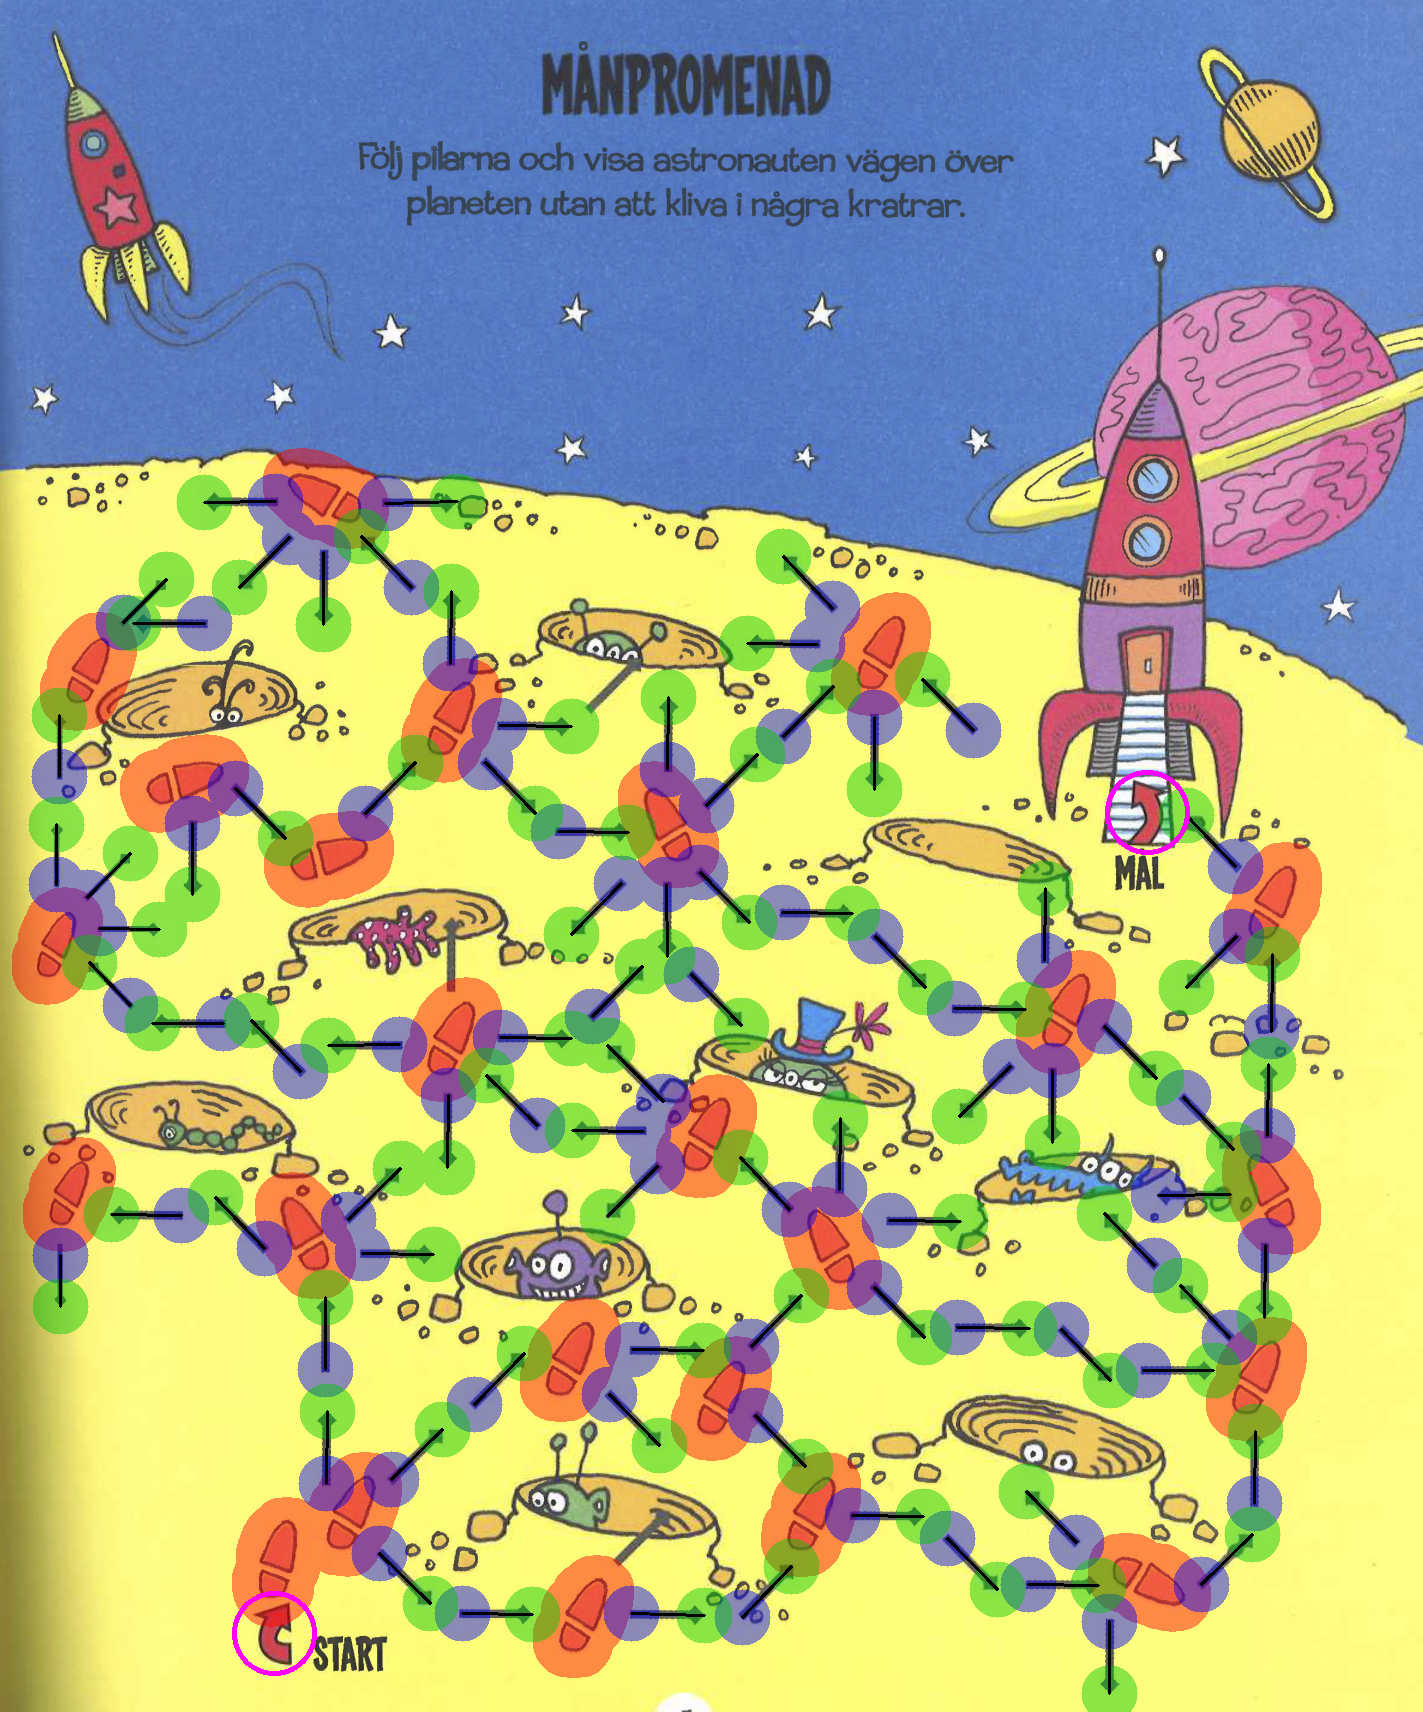
\includegraphics[width=\textwidth]{t6_15_grown_areas.png}
        \caption{Grown areas: footprints in red, tails in blue, heads in green}
    \end{subfigure}
    \begin{subfigure}{0.35\textwidth}
        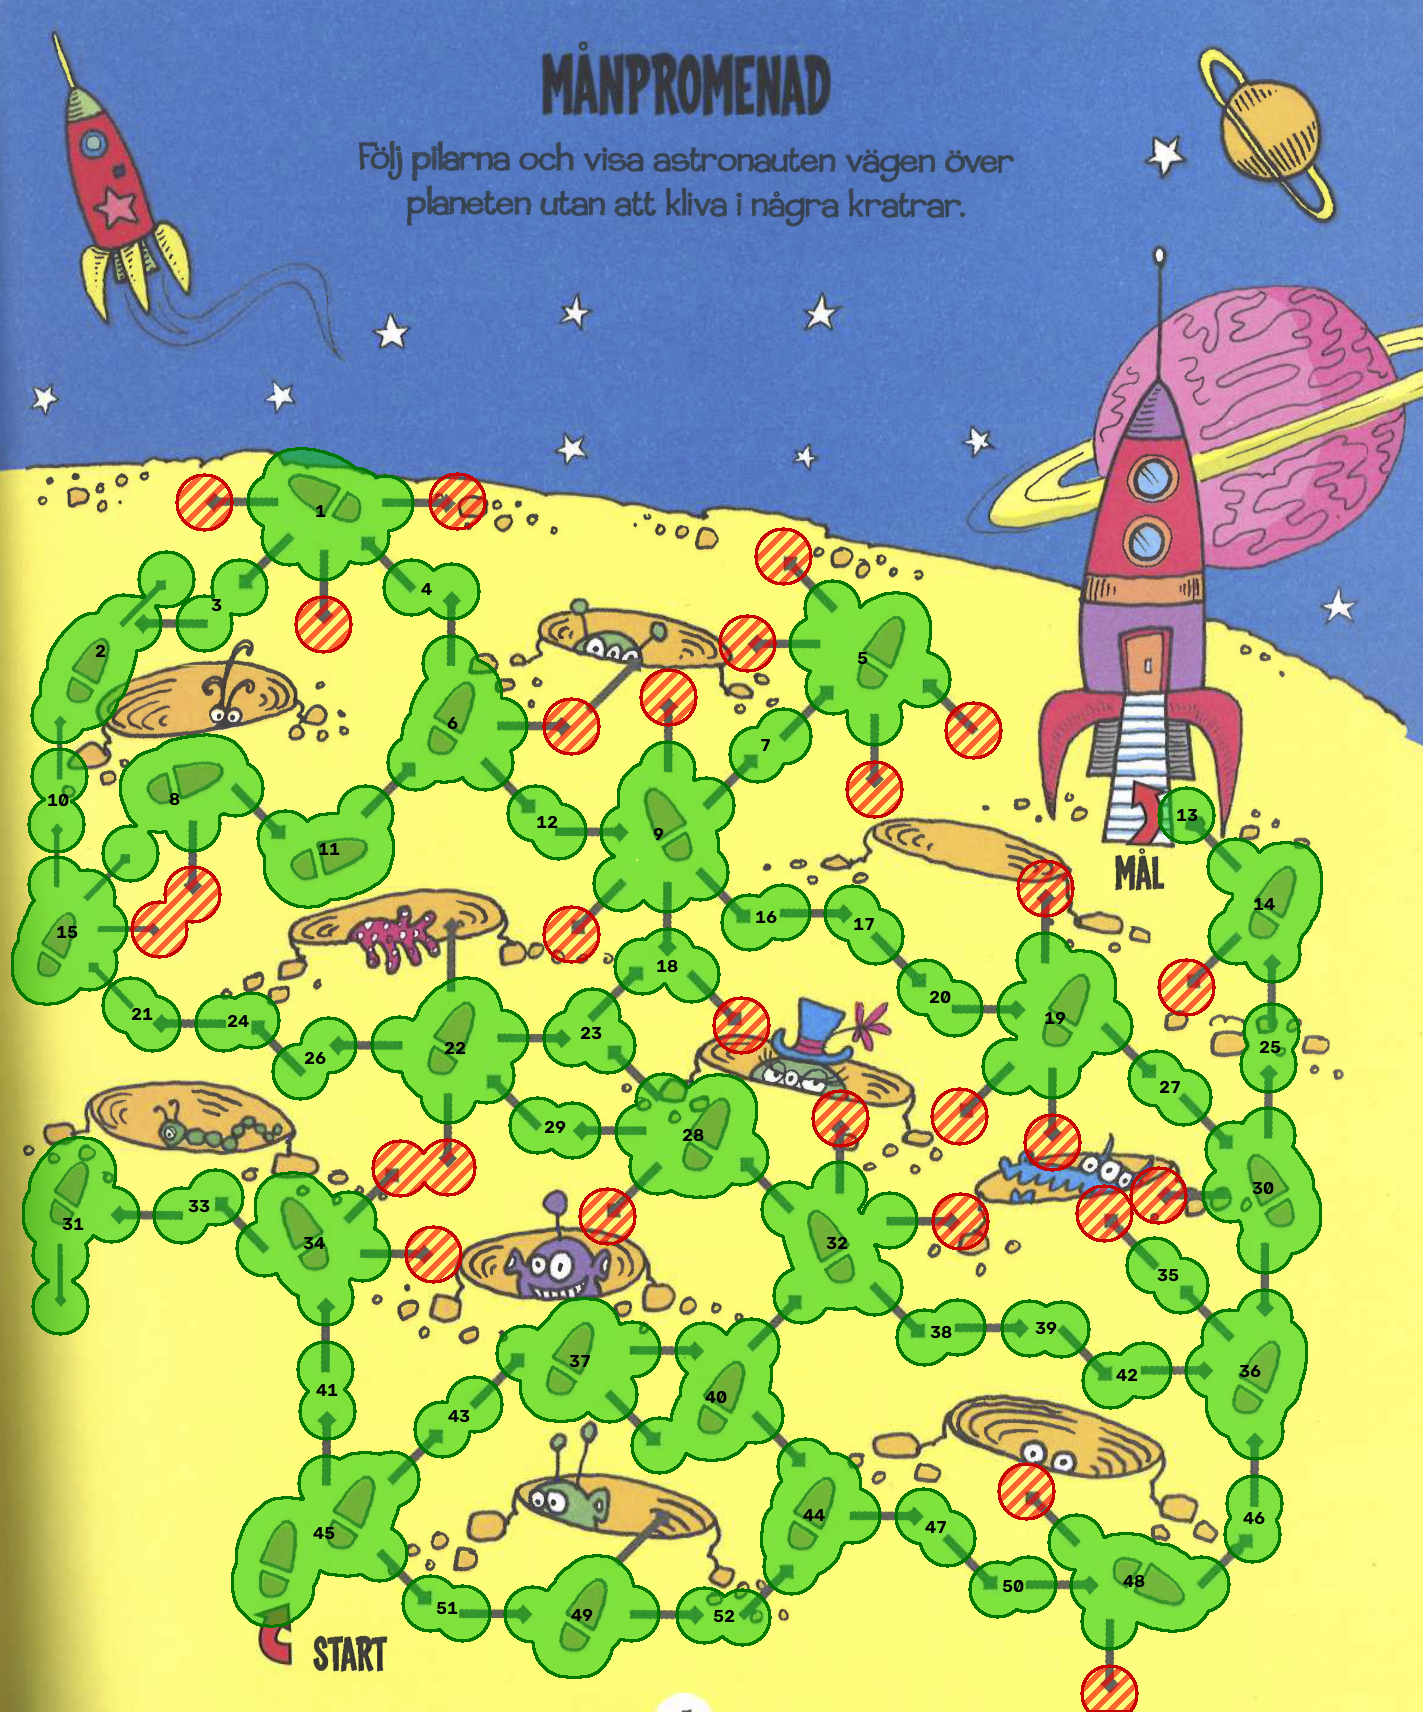
\includegraphics[width=\textwidth]{t6_16_nodes.png}
        \caption{Nodes in green, candidates that are not nodes with red stripes}
    \end{subfigure}
    \caption{The grown areas and the nodes.}
\end{figure}

\textbf{Graph and search.} Each arrow whose tail and head are in two different nodes gives a directed edge between them. The graph has 52 nodes and 57 edges. A breadth-first search from START finds the shortest path to MÅL, which is 25 steps long. The path follows the arrows in their direction and does not touch any crater.

\begin{figure}[H]
    \centering
    \begin{subfigure}{0.35\textwidth}
        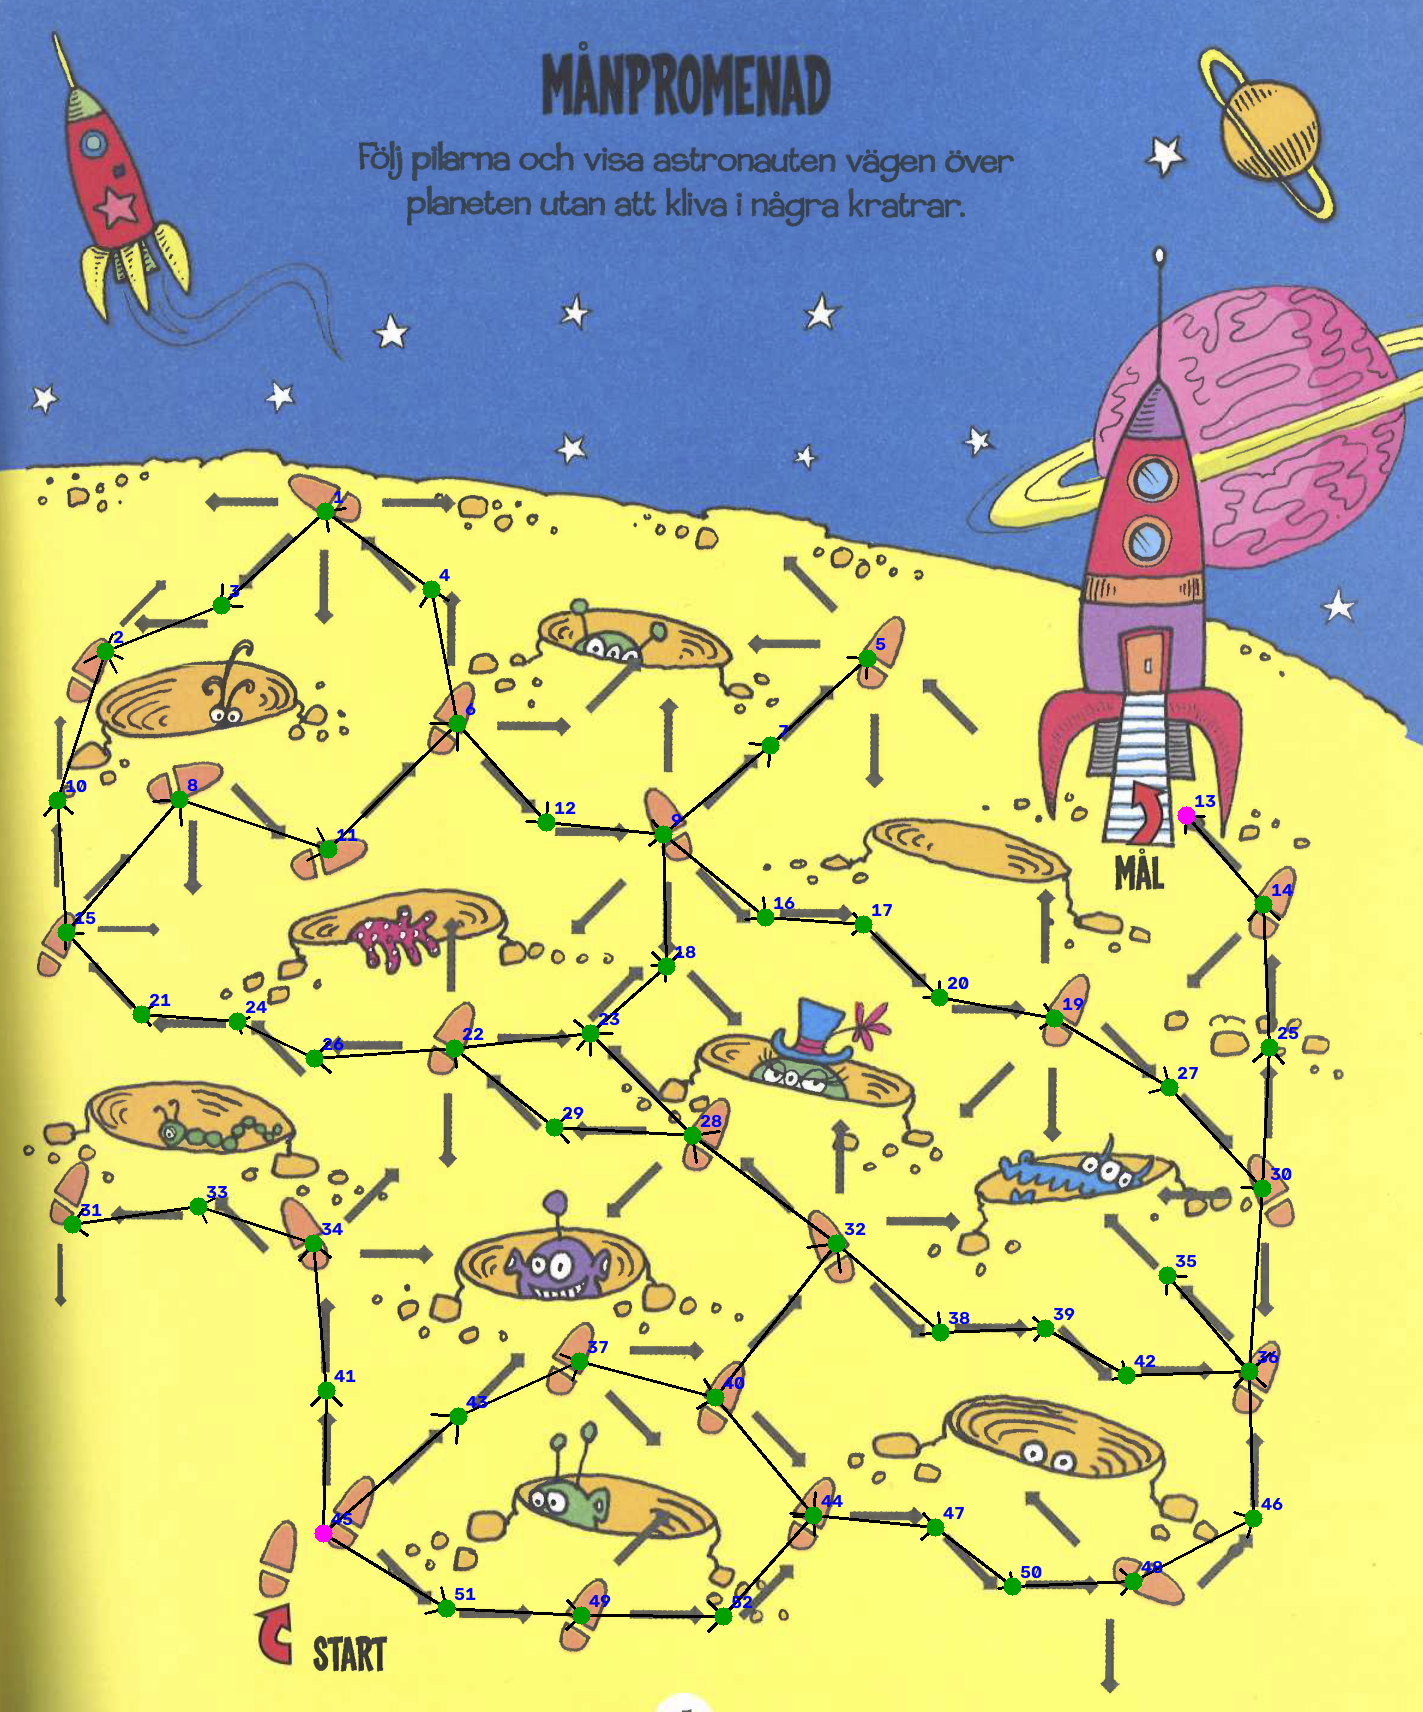
\includegraphics[width=\textwidth]{t6_17_graph.png}
        \caption{The graph}
    \end{subfigure}
    \begin{subfigure}{0.35\textwidth}
        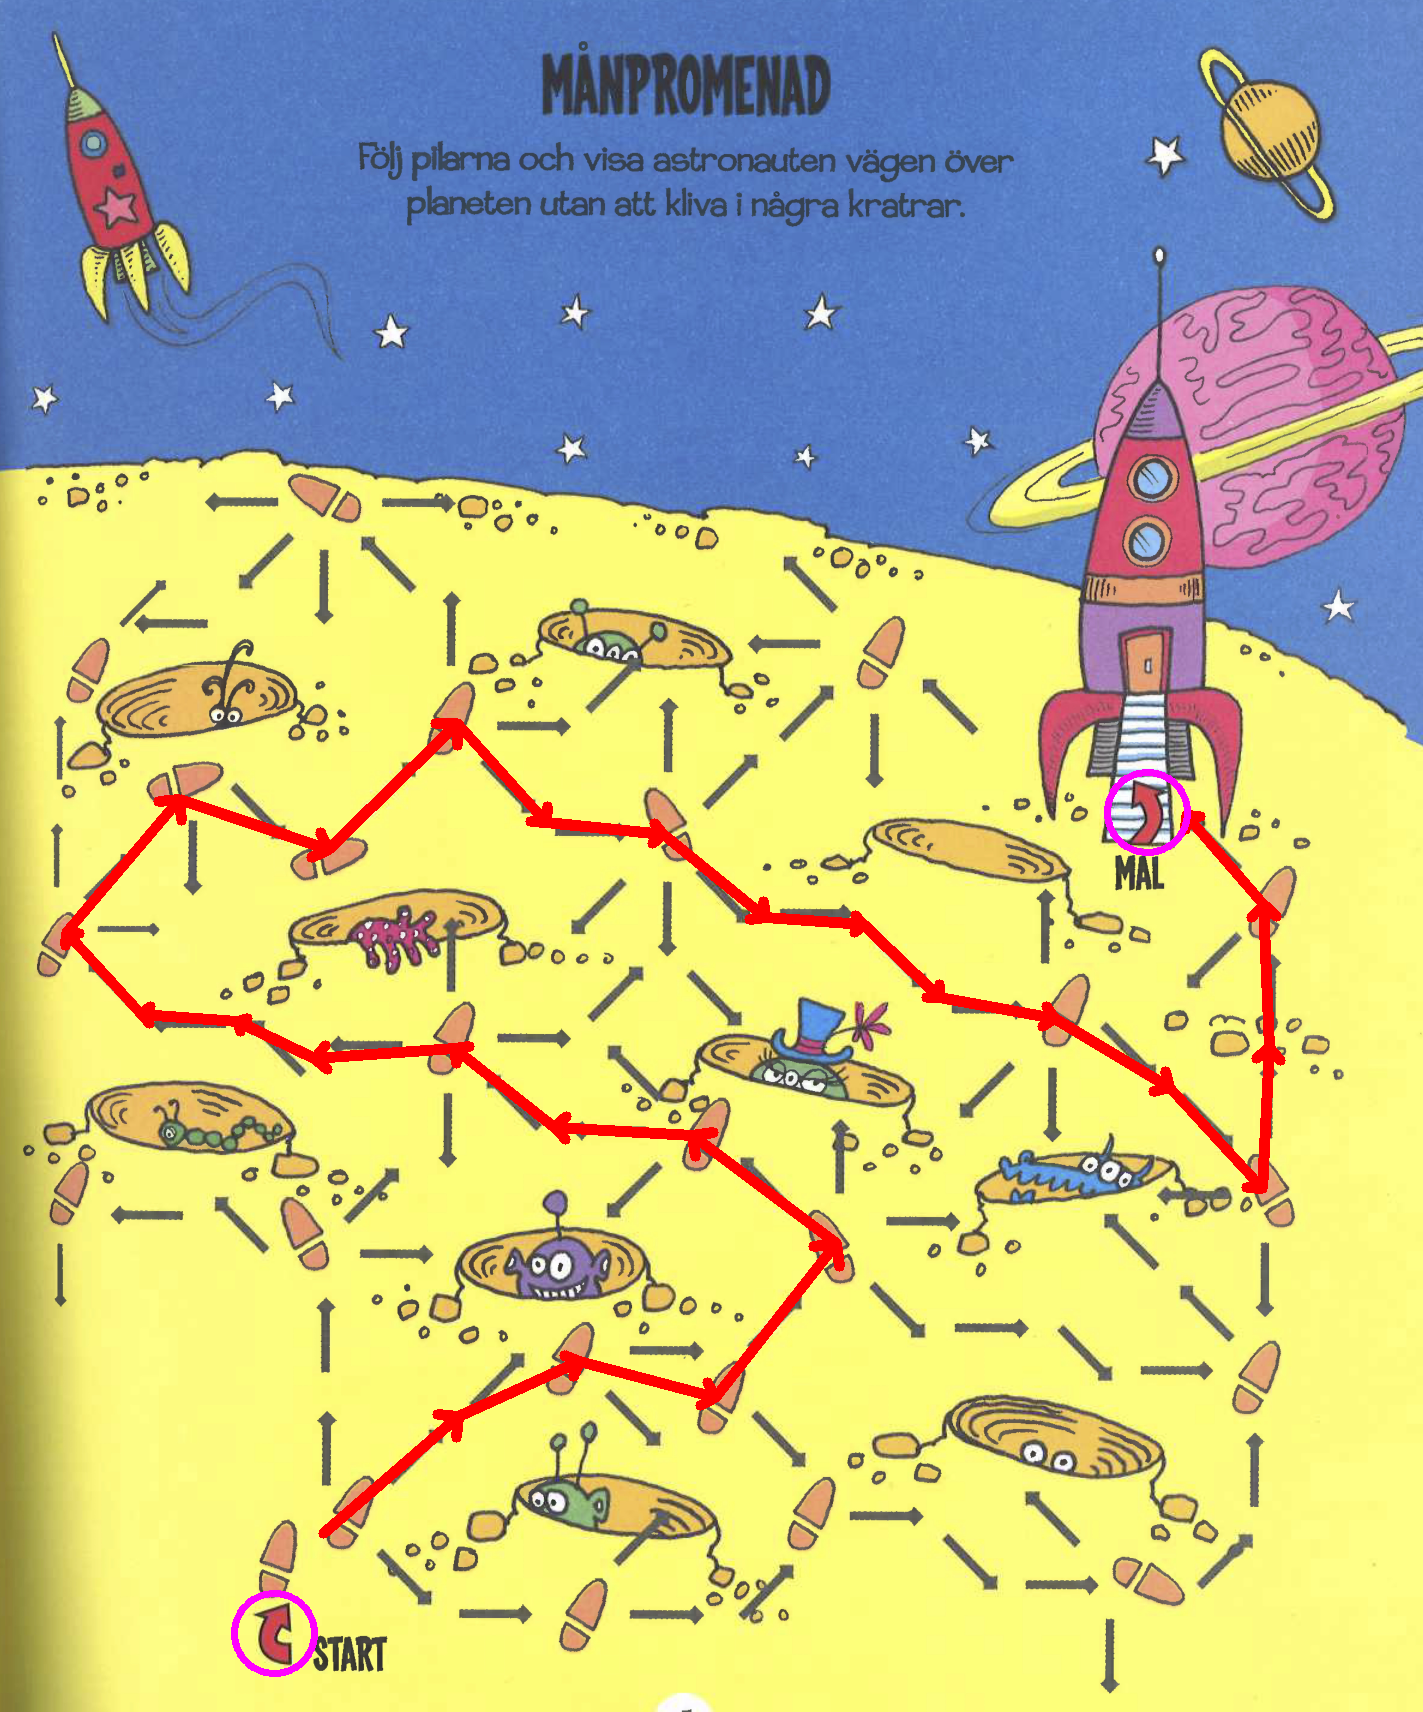
\includegraphics[width=\textwidth]{t6_18_path.png}
        \caption{The path from START to MÅL}
    \end{subfigure}
    \caption{The graph and the path found by the search.}
\end{figure}

\section*{References}

The code for all the tasks is available at \url{https://github.com/elinaRosato/FMAN20-home-exam}.

\end{document}
